% !TeX root = vpl.tex

\documentclass[11pt,a4paper,english]{report}
\usepackage[en]{../../vpl}
\graphicspath{{../../images/} {../../images/en/}}

\includeonly{vpl-brait}

\begin{document}
% !TeX root = vpl.tex

\thispagestyle{empty}

\begin{center}
\begin{Huge}
\begin{bfseries}
Primi passi nella Robotica
\end{bfseries}

con il

\begin{bfseries}
Robot Thymio-II
\end{bfseries}

e

\begin{bfseries}
L'Ambiente di programmazione Aseba/VPL
\end{bfseries}

\end{Huge}

\vskip 2cm

\begin{LARGE}
\href{http://www.weizmann.ac.il/sci-tea/benari/}{Moti Ben-Ari} e altri\\
\end{LARGE}
\bigskip
\begin{Large}
vedere \texttt{authors.txt} per dettagli
\end{Large}

\vskip 1cm

\begin{Large}
Versione 1.3{\textasciitilde}pre3 per \href{https://aseba.wikidot.com/en:downloadinstall}{Aseba 1.3.1}
\end{Large}

\end{center}

\vfill

\begin{center}
\copyright{}\  2013--14 by \href{http://www.weizmann.ac.il/sci-tea/benari/}{Moti Ben-Ari} e altri.
\end{center}

Questo lavoro è rilasciato sotto la licenza Creative Commons
Attribution-ShareAlike 3.0 Unported. Per vedere una copia della licenza, visitare
\url{http://creativecommons.org/licenses/by-sa/3.0/}
o inviare una lettera a Creative Commons, 444 Castro Street, Suite 900,
Mountain View, California, 94041, USA.

\begin{center}

\includegraphics[width=.2\textwidth]{../images/by-sa}
\end{center}

\newpage
\tableofcontents
\thispagestyle{empty}
\newpage
\setcounter{page}{1}

\chapter*{Preface}

\sect{What is a robot?}

You are riding your bicycle and suddenly you see that the street starts
to go uphill. You pedal faster to supply more power to the wheels so
that the bicycle won't slow down. When you reach the top of the hill and
start to go downhill, you squeeze the brake lever. This causes a rubber
pad to be pressed against the wheel and the bicycle slows down. When you
ride a bicycle, your eyes are \textit{sensors} that sense what is going
on in the world. When these sensors---your eyes---detect an
\textit{event} such as a curve in the street, you perform an
\textit{action}, such as moving the handlebar left or right.

In a car, there are sensors that \textit{measure} what is going on in
the world. The speedometer measures how fast the car is going; if you
see it measuring a speed higher than the limit, you might tell the
driver that he is going too fast. In response, he can perform an action,
such as stepping on the brake pedal to slow the car down. The fuel meter
measures how much fuel remains in the car; if you see that it is too
low, you can tell the driver to find a gas station. In response, he can
perform an action: raise the turn-signal lever to indicate a right turn
and turn the steering wheel in order to drive into the station.

The rider of the bicycle and the driver of the car receive data from the
sensors, decide what actions to take and cause the actions to be
performed. A \textit{robot} is a system where this process is carried out by a
computerized system, usually without the participation of a human.

\sect{The Thymio robot and the Aseba VPL environment}

The Thymio is a small robot intended for educational purposes
(\cref{fig.front}). The robot includes sensors that can measure light,
sound and distance, and can detect when buttons are touched and when the
robot's body is tapped. The most important action that it can perform is
to move using two wheels, each powered by its own motor. Other actions
include generating sound and turning lights on and off.

The name Thymio is used in this document to refer to the Thymio~II
robot.

Aseba is a programming environment for small mobile robots such as the
Thymio. VPL is a component of Aseba for \textit{visual programming} that
was designed to program Thymio in an easy way through event and action
blocks.

%\newpage

\sect{Overview of the tutorial}

For each chapter, we give the main topic, as well as lists of the event
and action blocks that are introduced. I suggest that you start with the
tutorial chapters on VPL basic mode. Then, you can study the tutorial on
advanced mode, or try some of the projects. The Parsons puzzles can be
tried whenever you feel the need to evaluate your knowledge of VPL.
Read the \cref{ch.next} when you are ready to leave VPL and work with
the more advanced Aseba Studio environment. The appendices contain
reference material that can be read as needed.

\subsection*{Part I: Tutorial}

\textbf{\cref{ch.intro,ch.colors}} are an essential
introduction to the robot, the VPL environment and its principal
programming construct: the event-actions pair.

\textbf{Events}: Buttons \hfill \textbf{Actions}: Top colors, bottom colors

\blkmed{event-buttons} \hfill \blkmed{action-colors-up} \quad \blkmed{action-colors-down}

\medskip

\textbf{\cref{ch.moving,ch.pet,ch.line}} present the events,
actions and algorithms for constructing autonomous mobile robots and
should be the core of any activity using Thymio and VPL.

\textbf{Events}: Buttons, front sensors, bottom sensors \hfill
\textbf{Actions}: Motors

\blkmed{event-buttons} \quad\blkmed{event-prox}\quad \blkmed{event-prox-ground} \hfill
\blkmed{action-motors}

\medskip

\textbf{\cref{ch.bells}} describes features of the robot that can
be fun to use but are not essential: sounds and shocks.

\textbf{Events}: Tap, clap \hfill \textbf{Actions}: Music, top colors,
bottom colors

\blkmed{event-tap} \quad \blkmed{event-clap} \hfill \blkmed{action-music}
\quad \blkmed{action-colors-up} \quad \blkmed{action-colors-down}

\medskip

\importantbox[Advanced mode]{VPL has a basic mode which supports
elementary events and actions that are easy for beginners to master. The
advanced mode of VPL supports more events and actions that require
experience to use. Explanations of the features of advanced mode
start in \cref{ch.time}.}

\medskip

\textbf{\cref{ch.time}} presents timed events. There is an action
to set a timer and when the timer expires, an event occurs.

\textbf{Events}: Timer expired \hfill \textbf{Actions}: Set timer

\blkmed{event-timer} \hfill \blkmed{action-timer}

\newpage

\textbf{\cref{ch.states,ch.counting}} explain state machines, which
enable the robot to perform different operations at different times.
States can also be used to perform elementary arithmetic like counting.

\textbf{Events}: State associated with an event \hfill \textbf{Actions}:
Change state

\blkmed{state-filter} \hfill \blkmed{action-states}

\medskip

\textbf{\cref{ch.angles}} describes how to use the accelerometers
in the Thymio robot.

\textbf{Events}: Accelerometer events

\blkmed{event-pitch} \quad \blkmed{event-roll}

\bigskip

\subsection*{Part II: Parsons puzzles}

\textbf{\cref{ch.parsons}} presents Parsons puzzles which are exercises
that you can use to check your knowledge of VPL.

\bigskip

\subsection*{Part III: Projects}

\textbf{\cref{ch.brait,ch.rabbit,ch.barcode,ch.sweep,ch.speed,ch.radar,ch.fa,ch.slow,ch.two}}
specify projects that you can design and implement on your own.
The VPL source is available in the archive, but I suggest that you work
on the projects before looking at the solutions.

\bigskip

\subsection*{Part IV: From visual to textual programming}

\textbf{\cref{ch.next}} points to the next step: using the
textual Studio environment which offers significantly more support for
developing robots than does the VPL environment.

%\informationbox{Reference material}{The appendices contains reference
%material that you will want to look at from time to time to learn about
%new featuers of VPL or to refresh your memory.}
\bigskip

\subsection*{Part V: Appendices}

\textbf{\cref{a.toolbar}} contains a description of the user
interface---the buttons on the toolbar.
%It also describes how to display dynamic feedback when a VPL program is run.

\textbf{\cref{a.blocks}} is a list of the event and
action blocks in both basic and advanced modes.

\textbf{\cref{a.tips}} provides guidance for teachers and
mentors of students. The first section suggests ways to encourage
exploration and experimentation. The next section focuses on good
programming practices. The final section lists some pitfalls that may be
encountered and offers hints on how to overcome them.

\textbf{\cref{a.tech}} describes techniques for working with the
sliders of the sensor and motor blocks.

\blkmed{event-prox-advanced} \quad \blkmed{event-prox-ground-advanced}


\sect{Reference cards}

You will find it useful to print out one or both of the VPL reference cards,
which are in the same zip file as this document and also available
at \href{https://www.thymio.org/en:visualprogramming}{https://www.thymio.org/en:visualprogramming}.

\begin{itemize}
\item A single page that summarizes the event and action blocks.
\item A two-sided page that can be folded to form a handy card.
It summarizes the VPL interface, the event and action blocks,
and includes example programs.
\end{itemize}

\sect{Installing Aseba}

To install Aseba, including VPL, go to
\href{https://www.thymio.org/en:start}{https://www.thymio.org/en:start}
and click on the icon for your system (Windows, Mac OS, etc.). Following
the instructions to download and install the software. The Aseba
installation includes both the VPL and the Studio (see \cref{ch.next})
development environments.

\chapter*{Versions 1.3 et 1.4}

La liste suivante est destinée aux lecteurs ayant déjà une certaine expérience avec VPL dans sa version précédente, Aseba 1.3; elle énumère les différences entre cette version et la 1.4.
Si vous n'avez jamais utilisé VPL auparavant, vous pouvez sauter cette section.

\textbf{Changements apportés aux blocs événement et action}

\begin{itemize}

\item L'apparence graphique des boutons des blocs a été modifiée, principalement dans le but d'intégrer
de nouvelles fonctionnalités.

\item Dans la 1.3, une case \emph{rouge} dans un bloc événement capteurs horizontaux déclanchait un événement
lorsque le capteur détectait un objet, alors qu'une case \emph{blanche} déclanchait un événement lorsqu'il n'y
avait pas d'objet en face du capteur.
Dans la 1.4, une case \emph{blanche} déclanche un événement quand le capteur mesure beaucoup de lumière réfléchie,
alors qu'une case \emph{noire} déclanche un événement lorsque le capteur mesure peu ou pas de lumière réfléchie
parce qu'il n'y a pas d'objet devant le capteur (pages~\pageref{p.proximity-colors1},~\pageref{p.proximity-colors2}).
Les capteurs du bas utilisent aussi les couleurs noir et blanc, au lieu de rouge et blanc,
mais le fonctionnement dans la 1.4 est identique à la 1.3, avec le noir au lieu du rouge.

\item En mode avancé, les seuils des capteurs peuvent être modifiés (page~\pageref{p.accel}).

\item En mode avancé, un événement permet de créer des événements accéléromètre en indiquant des valeurs pour les accéléromètres avant/arrière ou gauche/droite (page~\pageref{p.accel}).

\end{itemize}

\textbf{Modifications de l'interface utilisateur}

\begin{itemize}

\item Des actions multiples associées au même événement (page~\pageref{p.multiple}).

\item Les blocs et les paires événement-actions peuvent être copiées (page~\pageref{p.copy-pairs}).

\item Les captures d'écran des programmes VPL peuvent être exportés en plusieurs formats (page~\pageref{p.proximity-sensitivity}).

\item Les boutons annuler/rétablir ont été ajoutés (page~\pageref{p.undo}).

\item Le bouton Lancer clignote en vert lorsque le programme a été modifié (page~\pageref{p.blink}).

\item Il n'est désormais plus possible de modifier la palette de couleurs de VPL.

\end{itemize}

% !TeX root = vpl.tex

\part{Tutorial}

\chap{Your First Robotics Project}\label{ch.intro}

\sect{Getting to know your Thymio}

\Cref{fig.front} shows the front and top of Thymio. On the top you
can see the center circular button (\textcolor{blue}{A}) and four
directional buttons (\textcolor{blue}{B}). Behind the buttons, the green
light (\textcolor{blue}{C}) shows how much charge remains in the
battery. At the back are the top lights (\textcolor{blue}{D}), which
have been set to red in this picture. There are similar lights on the
bottom (see \cref{fig.bottom}). The small black rectangles
(\textcolor{blue}{E}) are sensors which you will learn about in
\cref{ch.pet}.

\begin{figure}[h]
\begin{center}
\gr{front}{.8}
\caption{The top and front of the Thymio robot}\label{fig.front}
\end{center}
\end{figure}

\sect{Connect the robot and run VPL}

Connect your Thymio robot to your computer with a USB cable; the robot
will play a sequence of tones. If the robot is turned off, turn it on by
touching the center button for a few seconds until you hear the tones.
Run VPL by double-clicking on the icon \blksm{thymiovpl} on your
computer.

\importantbox[Small images]{When a small image appears
in the text, a larger image is displayed in the margin.}

VPL may connect automatically to your robot. If not, the window shown in
\cref{fig.connect} will be displayed. Check the box next to \bu{Serial},
click on \bu{Thymio Robot} below it, select a language, and then click
\bu{Connect}. Depending on the configuration of your computer and
operating system, there may be several entries in this table and the
data following \bu{Thymio Robot} may be different from what is shown in
the Figure.

\trickbox{It is also possible to access VPL from Aseba Studio, the
text-based programming environment through the VPL plugin found in the
\textit{Tool} area at the bottom left of the screen.}

\begin{figure}
\begin{center}
\gr{connect}{.4}
\caption{Connect to Thymio through serial port (USB)}\label{fig.connect}
\end{center}
\end{figure}

\sect{Wireless Thymio}

The Thymio robot comes in a wireless version that does not need to be connected
to a computer in order to load programs. The wireless robot comes with a small object called a \emph{dongle}:

\gr{dongle}{.4}

Plug the dongle into a USB socket on your computer, turn the robot on and start VPL, as described above. When you see the connection window (Figure~\ref{fig.connect}) select the line \bu{Thymio-II Wireless (COM15)}.

\importantbox{You need to use the USB cable to charge the Thymio (Figure~\ref{fig.back}).}


\sect{The VPL user interface}

The user interface of VPL is shown in Figure~\ref{fig.vplgui}.
There are six areas in the interface:
\begin{enumerate}[noitemsep,nosep]
\item A toolbar with buttons for opening, saving, running a program, etc.
\item A program area where programs for controlling the robot are constructed.
\item A message area which displays error messages if the program is not
well-formed.
\item A column with event blocks for constructing your program.
\item A column with action blocks for constructing your program.
\item The translation of the program into AESL, the textual language of Aseba.
\end{enumerate}

\plainfloat
\begin{figure}[h]
\gr{gui}{1}
\caption{The VPL window}\label{fig.vplgui}
\end{figure}
\framedfloat

\informationbox{The VPL toolbar}{\cref{a.toolbar} contains a
description of all the buttons in the VPL toolbar.\\
Look at it occasionally until you have learned how to use them.}

\informationbox{To go further}{ When you construct a program using VPL, the
translation of the program into the textual programming language AESL
appears in the right part of the window. It is the AESL program that is
actually run by the robot. \cref{ch.next} explains these translations.
The webpage \href{https://www.thymio.org/en:asebausermanual}{https://www.thymio.org/en:asebausermanual} contains learning and reference materials on AESL and its Studio environment.}

\sect{Write a program}

When you start VPL, a blank program area is displayed.

If, after having built a piece of program, you wish to clear the content
of the program area, click \blksm{new} (\bu{New}).

A program in VPL consists of \emph{event-actions pairs}, each
constructed from an event block and one or more action blocks. For
example, the pair: \blkc{e-a-pair} causes the top light of the robot to
display red when the front button is touched.

\importantbox[Meaning of an event-actions pair]{\centering When the event
occurs, the associated actions are run.}

The program area will initially contain an empty frame for an
event-actions pair: \blkc{empty-frame} To bring a block to the program
area from the columns (areas 4 and 5 of \cref{fig.vplgui}), press and
hold the left mouse button and drag the block to a dashed square. When the
block is over the square, release the mouse button, dropping the block
into its place.

\importantbox{The technique just described is call
\emph{drag-and-drop} and is widely used in the user interface of
programs.}

Start by bringing the button event block \blksm{event-buttons} into the
left side of the empty frame. You will get a message inviting you to add
an action block. Drag the top color action block
\blksm{action-colors-up} and drop it into the right side of the frame. You have
constructed an event-actions pair!

Next, we have to modify the event and the action to do what we want. For
the event, click on the front button (the top triangle); it will turn
red: \blkc{forward} This specifies that an event will occur when the
\textit{front button} of Thymio is touched.

The color action block contains three \emph{sliders}---colored bars with
a white square---one for each of the primary colors red, green, blue.
Drag a white square to the right and then back to the left, and you will
see that the background color of the block changes. All colors can be
made by mixing these three primary colors: red, green and blue. Move
the red slider until the square is at the far right, and move the green
and blue sliders until they are at the far left. The color will be all
red with no blue nor green: \blkc{red}

\sect{Save the program}

Before running the program, save it on your computer. Click on the
button \blksm{save} (\bu{Save}) in the toolbar. You will be asked to
give the program a name; choose a name that will help you remember what
the program does, perhaps, \bu{display-red}. Choose the location where
you want to save your program and click on \bu{Save}.


\importantbox[Save frequently]{When you modify a program, click
\bu{Save} frequently so that you don't lose your work if something
happens to the computer.}


\sect{Run the program}

To run the program, click on \blksm{run} (\bu{Run}) in the toolbar.
Touch the front button on the robot; the light on top of the robot
should change to red.

\informationbox{Congratulations!}{You have created and run your
first program. Its behavior is:\\ \textbf{When you touch the forward
button of the Thymio, it becomes red.}}

If you need to stop the VPL program, click \blksm{stop} (\bu{Stop}) .
This is important when you run a program that causes the robot to move,
but the program does not have an event-actions pair to stop the motors.

\sect{Turn the robot off}

When you have finished working with the Thymio robot, turn it
off by touching and holding the center button for a few seconds until
you hear a sequence of tones. The battery will
continue charging as long as it is connected to a working computer. A
red light next to the USB cable connector means that the robot is
charging; it turns blue when the charging is completed (\cref{fig.back}).
You can disconnect the cable when you are not using the robot.

\trickbox{To charge the robot faster, use a mobile phone
charger with a micro-USB connector.}

\begin{figure}
\begin{center}
\gr{back}{.6}
\caption{The back of the Thymio showing the USB cable and the
 charging light}\label{fig.back}
\end{center}
\end{figure}

Should the USB cable disconnect during programming, VPL will wait for
the connection to be made again. Check both ends of the cable, reconnect
and see if VPL is working. If you have a problem, you can always close
VPL, reconnect the robot and open VPL again.

\sect{Modify a program}

\begin{itemize}

\item To delete an event-actions pair, click \blkxsm{x} at the top-right
of the pair.

\item To add an event-actions pair, click \blkxsm{plus} available below
an existing pair.

\item To move an event-actions pair to another position in the program,
drag and drop it at the desired location.

\item To copy an event-actions pair to another position in the program,
press and hold the \bu{Ctrl} and then use the mouse to drag and drop the
pair at the desired location.\label{p.copy-pairs}\footnote{On Mac
OS, the \bu{Command} button is used instead of \bu{ctrl}.}

\end{itemize}

\informationbox{The blinking \bu{Run} button}{When you modify a program,
the \bu{Run} button blinks blue and green to remind you that you need to
click the button to load the modified program into the Thymio
robot.\label{p.blink}}

If you want to experiment with a modification but not lose an existing
program, you can create a copy of the existing program by clicking
\blksm{saveas} (\bu{Save as}) and giving a new file name.

\sect{Open an existing program}

Suppose that you have saved your program and turned off the robot and
the computer, but later you wish to continue to work on the program.
Connect the robot and run VPL as described previously. Click on
\blksm{open} (\bu{Open}) and select the program you want to open, for
example, \bu{display-red}. The event-actions pairs of the program will
be displayed in the program area, and you can continue working on it.

\sect{The current event-actions pair}

When you click on an event-actions pair, it will be displayed with a
yellow background. This will also occur when you enter an event or
action block in an empty pair:

\begin{center}
\begin{tabular}{c@{\hspace{.1\textwidth}}c}
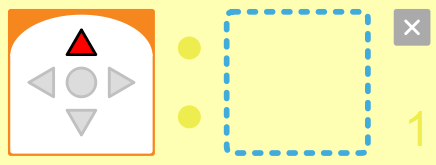
\includegraphics[width=.3\textwidth,keepaspectratio=true]{event-action-pair-yellow1}
&
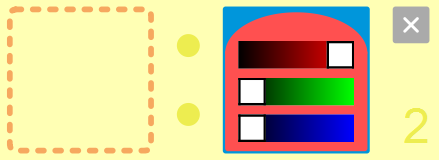
\includegraphics[width=.3\textwidth,keepaspectratio=true]{event-action-pair-yellow2}
\end{tabular}
\end{center}

The left gold-colored square is the space for the event; the right
blue-colored square is for the first (or only) action. The pair with the
yellow background is called the \emph{current} pair.

\informationbox{Quick entering of a block}{If you click on an event or action block, it will be
automatically placed in the program area in the current
event-actions pair.}


\chap{Changer les couleurs}\label{ch.colors}

\sect{Colorer Thymio}

Créons un programme qui affiche deux couleurs différentes sur le dessus de Thymio lorsque les boutons avant ou arrière sont touchés, et deux autres couleurs sur le dessous et les côtés de Thymio lorsque les boutons gauche ou droite sont touchés.

{\raggedleft \hfill Programme: \bu{colors.aesl}}

Nous avons besoin de quatre paires événement-actions.
Il y a quatre événements --- toucher l'un des quatre boutons --- et une action couleur est associée avec chaque événement.
Notez la différence entre le bloc \blksm{action-colors-up} et le bloc \blksm{action-colors-down}.
Le premier des deux change la couleur affichée sur le dessus de Thymio alors que le deuxième change la couleur affichée sur le dessous et sur les côtés.
Le deuxième bloc a deux marques noires qui représentent les roues du robot et un point blanc qui représente le point d'appui à l'avant du robot (\cref{fig.bottom}).

Ce programme est illustré sur la \cref{fig.colors}.

\begin{figure}
\gr{colors1}{.35}
\caption{Changer de couleur quand un bouton est touché}\label{fig.colors}
\end{figure}

Quelles couleurs seront affichées?
Pour les premières trois actions, le \textit{slider} d'une couleur a été glissé tout à droite alors que les autres sont restés à gauche.
Ces actions affichent donc respectivement purement du rouge, du bleu et du vert.
L'action associée avec le bouton gauche mixe du rouge et du vert, ce qui produit donc du jaune.
Vous pouvez voir que le fond du bloc change de couleur quand on déplace les \textit{sliders}, ce qui vous montre de quelle couleur sera Thymio!

Lancez le programme \blksm{run} et touchez les boutons pour changer la couleur du robot.
La \cref{fig.front} montre Thymio allumé en rouge sur le dessus et la \cref{fig.bottom} montre Thymio allumé en vert sur le dessous.

\exercisebox{\thechapter.1}{
Expérimentez avec les \textit{sliders} pour voir quelles couleurs peuvent être affichées.
}

\trickbox[Information]{
En mixant ensemble du rouge, du vert et du bleu, vous pouvez créer n'importe quelle couleur (\cref{fig.cube}) !
}

\begin{figure}
\gr{color-cubes}{.85}
\caption{Le cube des couleurs rouge-vert-bleu (RVB)}\label{fig.cube}
\end{figure}

%\sect{Éteindre les lumières}
\sect{Plusieurs actions associées à un même événement}

Modifions maintenant le programme pour que les lumières s'éteignent lorsque le bouton central est touché.
Deux actions doivent avoir lieu lors d'un même événement --- le bouton du milieu est touché.
Il est possible d'associer \emph{deux} actions à un événement
dans une paire événement-actions.
Après avoir inséré l'événement et la première action (l'action couleur du haut), un nouveau cadre gris apparaîtra à droite de l'action:

\blkc{multiple-outline}

Vous pouvez maintenant glisser-déposer l'action couleur du bas 
dans ce cadre.
Vous obtiendrez une paire avec un événement et deux actions:\label{p.multiple}

\blkc{colors-multiple}

{\raggedleft \hfill Programme: \bu{colors-multiple.aesl}}

%\importantbox[De multiples paires événement-actions]{
N'oubliez pas de lancer le programme en cliquant sur l'icône \blksmpure{run}.
À l'avenir, il sera implicite qu'il vous faudra lancer chaque programme en cliquant sur cet icône, nous ne vous le dirons plus.

\bigskip

\importantbox[Les règles des paires événement-actions]{
\begin{itemize}[noitemsep,nosep,leftmargin=*]
\item Lorsqu'un programme est lancé, toutes les paires événement-actions sont actives.
\item Il est possible d'avoir plusieurs paires événement-actions avec le même événement mais il faut que les paramètres associés soient différents.
Vous pouvez par exemple avoir plusieurs paires avec l'événement bouton à condition que les combinaisons de boutons soient différentes entre les différents blocs événement.
\item Si les événements sont absoluement identiques dans plusieurs paires, VPL vous indiquera qu'il y a une erreur (zone 3 dans la \cref{fig.vplgui}).
Vous ne pourrez pas lancer le programme tant qu'il y a des erreurs.
\end{itemize}
}

\chap{Los, beweg dich}\label{ch.moving}

\sect{Vorwärts und rückwärts fahren}

Thymio hat zwei Motoren mit denen er seine zwei Räder unabhängig voneinander antreiben kann. Beide Motoren können vorwärts und rückwärts drehen. Dadurch kann der Roboter vorwärts und rückwärts fahren. Wir wollen uns mit einem kleinen Projekt befassen, um mehr über die Motoren zu lernen.

Der Aktions-Block für die Motoren \blksm{action-motors} zeigt ein kleines Bild des Roboters in der Mitte mit zwei Schiebereglern links und rechts. Mit den beiden Balken können Sie die Geschwindigkeit der beiden Motoren einstellen, mit dem linken Balken die des linken Motors und mit dem rechten Balken die des rechten Motors. Wenn das weisse Quadrat in der Mitte ist (vertikal), dreht der Motor nicht.  Sie können die Geschwindigkeit ändern, indem Sie das weisse Quadrat verschieben. Schiebt man das Quadrat nach oben, dreht der Motor vorwärts --- je weiter oben, desto schneller; schiebt man es nach unten, dreht der Motor entsprechend rückwärts.

Erstellen Sie ein Programm, um den Roboter vorwärts fahren zu lassen, wenn der Vorwärts-Kopf gedrückt wird und rückwärts, wenn der Rückwärts-Knopf gedrückt wird.

{\raggedleft \hfill Beispielprogramm \bu{moving.aesl}}

Wir brauchen zwei Ereignis-Aktions-Paare:
%(\cref{fig.nostop}).

%\begin{figure}
\begin{center}
\gr{no-stop-motors}{.3}
%\caption{Moving forward or backwards}\label{fig.nostop}
\end{center}
%\end{figure}

Ziehen Sie die Ereignis- und Aktions-Blöcke in die Programmierumgebung und stellen Sie für beiden Motoren die Schieberegler auf halbe Geschwindigkeit ein. Dies indem Sie die Quadrate für vorwärts fahren halb nach oben und für rückwärts fahren halb nach unten verschieben.

Führen Sie das Programm aus und drücken Sie die Knöpfe, um den Roboter vorwärts- und rückwärts fahren zu lassen. 

\sect{Den Roboter anhalten}

\textbf{Hilfe!} Ich kann den Roboter nicht mehr stoppen!

Klicken Sie auf das Symbol \blksm{stop}, um den Roboter zu stoppen.

Wir wollen diese Problem beheben, indem wir ein neues Ereignis-Aktions-Paar
hinzufügen: \blkc{stop-motors}
Dieses soll die Motoren stoppen, wenn der mittlere Knopf gedrückt wird. Wenn Sie den Motoraktionsblock in die Programmierumgebung ziehen, sind die Schieberegler in der Mitte, was die Motoren ausschaltet und den Roboter anhalten lässt.

\sect{Nicht vom Tisch fallen!}

Wenn der Roboter auf dem Boden fährt, kann er im schlimmsten Fall in eine Wand
fahren oder sein USB-Kabel herausziehen. Aber wenn der Roboter auf einem Tisch
fährt, kann er auf den Boden fallen und kaputt gehen! Wir wollen den Roboter so
programmieren, dass er anhält, sobald er die Tischkante erreicht.

\warningbox{Wenn der Roboter auf einem Tisch fährt, muss man bereit sein, um ihn aufzufangen, falls er hinunterfällt.}

Drehen Sie Ihren Thymio auf den Rücken. Nun sehen Sie, dass er unten zwei
kleine, schwarze Rechtecke mit optischen Elementen hat (\cref{fig.bottom}).
Das sind \emph{Bodensensoren}. Diese senden Infrarotlichtimpulse aus und messen wie viel Licht reflektiert wird. 
Auf einem hellen Tisch wird viel Licht reflektiert. Fährt der Roboter über die Tischkante wird wenig Licht reflektiert. Tritt dies ein, möchten wir, dass der Roboter stoppt.

\trickbox{Benutzen Sie einen hellen Tisch aber keinen aus Glas, da von diesem kein Licht reflektiert wird. Thymio kann dann nicht erkennen, ob er auf einem Tisch ist oder nicht.}

Ziehen Sie das Bodensensor-Ereignis \blksm{event-prox-ground}
in Ihr Programm. Oben hat dieser Block zwei kleine Quadrate. Wenn Sie sie anklicken, werden sie weiss mit rotem Rand, schwarz und dann wieder grau. Die Farben haben verschiedene Bedeutungen:

\begin{itemize}

\item \textbf{Grau}: Der Sensor wird nicht beachtet.

\item \textbf{Weiss}: Das Ereignis tritt ein, wenn viel Licht reflektiert wird. \label{p.proximity-colors1} Links vom weissen Feld wird ein kleiner roter Punkt dargestellt; dies nimmt Bezug auf das rote Licht neben dem Sensor, das leuchtet, wenn der Sensor etwas entdeckt hat.\footnote{Das weisse Quadrat hat einen roten Rand, der daran erinnert, dass das Ereignis eintrifft, wenn die Lichter neben dem Sensor aufleuchten.}

\item \textbf{Schwarz}: Das Ereignis tritt ein, wenn es wenig oder kein reflektierendes Licht gibt.

\end{itemize}

%\trickbox[Information]{The gray, red and white colors used in a block
%are arbitrary and others could have been chosen.}

Damit der Roboter an der Tischkante anhält (wo es nur geringe Reflektion von Licht gibt) klicken Sie beide Quadrate bis sie schwarz werden.
Erstellen Sie das folgende Ereignis-Aktions-Paar: \blkc{dont-fall}

\begin{figure}
\begin{center}
\gr{bottom}{0.6}
\caption{Thymios Unterseite mit den beiden Bodensensoren}\label{fig.bottom}
\end{center}
\end{figure}

Stellen Sie den Roboter in der Nähe der Tischkante auf (auf die Tischkante ausgerichtet) und betätigen Sie den vorderen Knopf. Der Roboter sollte sich auf die Kante zu bewegen und anhalten, bevor er vom Tisch fällt. 

\bigskip

\exercisebox{\thechapter.1}{ Experimentieren Sie mit der Geschwindigkeit. Gelingt es dem Roboter bei Höchstgeschwindigkeit doch noch rechtzeitig anzuhalten? Falls nicht: ab welcher Geschwindigkeit fällt er vom Tisch? Kann man den Roboter auch im Rückwärtsgang davon abhalten, vom Tisch zu fallen?}

\bigskip

\warningbox{Als wir dieses Programm getestet haben, \emph{ist} der Roboter vom Tisch gefallen. Der Grund war, dass der Tisch eine abgerundete Kante hatte; sobald die fehlende Reflektion erkannt wurde, war es schon zu spät und der Roboter kippte nach vorne, verlor an Stabilität und viel vom Tisch.}

\chap{Ein Roboter als Haustier}\label{ch.pet}

Einen Roboter mit unabhängigem Verhalten nennen wir einen \emph{autonomen Roboter} und wir verbinden mit ihm Eigenschaften von lebenden Geschöpfen wir Katzen und Hunden. Das Verhalten wird erreicht durch \textit{Rückkoppelung}: der Roboter nimmt die Umgebung über ein Ereignis wahr und passt sein Verhalten über Aktionen an.

\sect{Der Roboter gehorcht}

Zuerst lehren wir den Roboter, uns zu gehorchen. Und zwar so, dass er sich normalerweise nicht bewegt; wenn er aber eine Hand vor sich wahrnimmt, soll er
auf diese Hand zu fahren.

{\raggedleft \hfill Beispielprogramm \bu{obeys.aesl}}

Der Roboter hat vorne fünf und hinten zwei horizontale Distanzsensoren.
Diese sind ähnlich aufgebaut, wie die Bodensensoren auf der Unterseite des Roboter, die wir in \cref{ch.moving} benutzt haben. Wenn Sie Ihre Hand langsam näher an die Sensoren des Roboters heranführen, leuchtet ein kleines, rotes
Licht neben dem Sensor auf und zeigt so an, dass die Hand erkannt wurde (\cref{fig.detect}).

\begin{figure}
\begin{center}
\gr{detect}{.5}
\caption{Thymios Vorderseite. Zwei Sensoren erkennen die Finger.}\label{fig.detect}
\end{center}
\end{figure}

Der Block \blksm{event-prox} wird gebraucht, um zu erfahren, ob etwas nahe am Sensor ist oder nicht. In beiden Fälle tritt ein Ereignis ein. Die schmalen, grauen Quadrate (fünf vorne und zwei hinten) können wahrnehmen, wann ein Ereignis stattfindet. 
Indem auf ein Quadrat gedrückt wird, ändert sich dieses von grau auf weiss, 
von weiss auf schwarz und zurück auf grau.
Die Bedeutung der Farben ist für diesen Block sind:

\begin{itemize}
	\item \textbf{Grau}: Der Sensor wird nicht beachtet.
	\item \textbf{Weiss}: Eine Aktion wird ausgelöst, falls ein Objekt im Bereich des Sensors erkannt wird.
	\item \textbf{Schwarz}: Eine Aktion wird gestartet, falls \emph{kein} Objekt im Bereich des Sensors erkannt wird.
\end{itemize}

Wenn Sie ein Ereignis auslösen wollen, wenn ein Objekt nahe beim Sensor ist, verwenden Sie ein weisses Quadrat, weil dann das Objekt viel Licht reflektieren wird. Wollen Sie andererseits ein Ereignis auslösen, wenn \emph{kein} Objekt in der Nähe des Sensors ist, verwenden Sie ein
schwarzes Quadrat, da dort nur wenig Licht reflektiert wird.

Um das gewünschte Verhalten zu implementieren, müssen wir zwei Ereignis-Aktions-Paare verwenden (\cref{fig.follow-hand}). Im ersten Paar ist der mittlere Frontsensor schwarz und die damit verbundene Aktion ist, dass die Motoren ausgeschaltet sind. Wenn also der Roboter kein Objekt erkennt, wird er sich nicht bewegen, bzw. anhalten, falls er in Bewegung war. Im zweiten Paar ist der mittlere Frontsensor weiss und die Schieberegler des Motorblocks sind beide vorne in Richtung Spitze; wenn also eine Hand vor dem mittleren Sensor erkannt wird, tritt das Ereignis ein und der Roboter setzt sich relativ rasch in Bewegung. 

\begin{figure}
\begin{floatrow}
	\ffigbox
	{\caption{Bewegung auf Hand zu}\label{fig.follow-hand}}
	{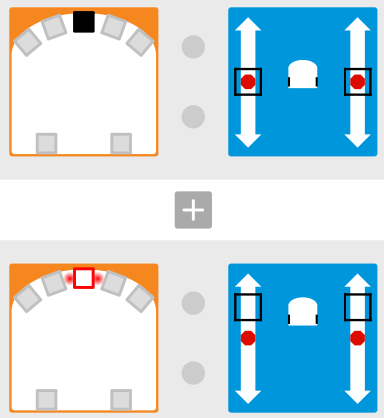
\includegraphics[width=.4\textwidth]{likes-forward}}
	\ffigbox
	{\caption{Ein Bulldozer mit Raupen}\label{fig.bull}}
	{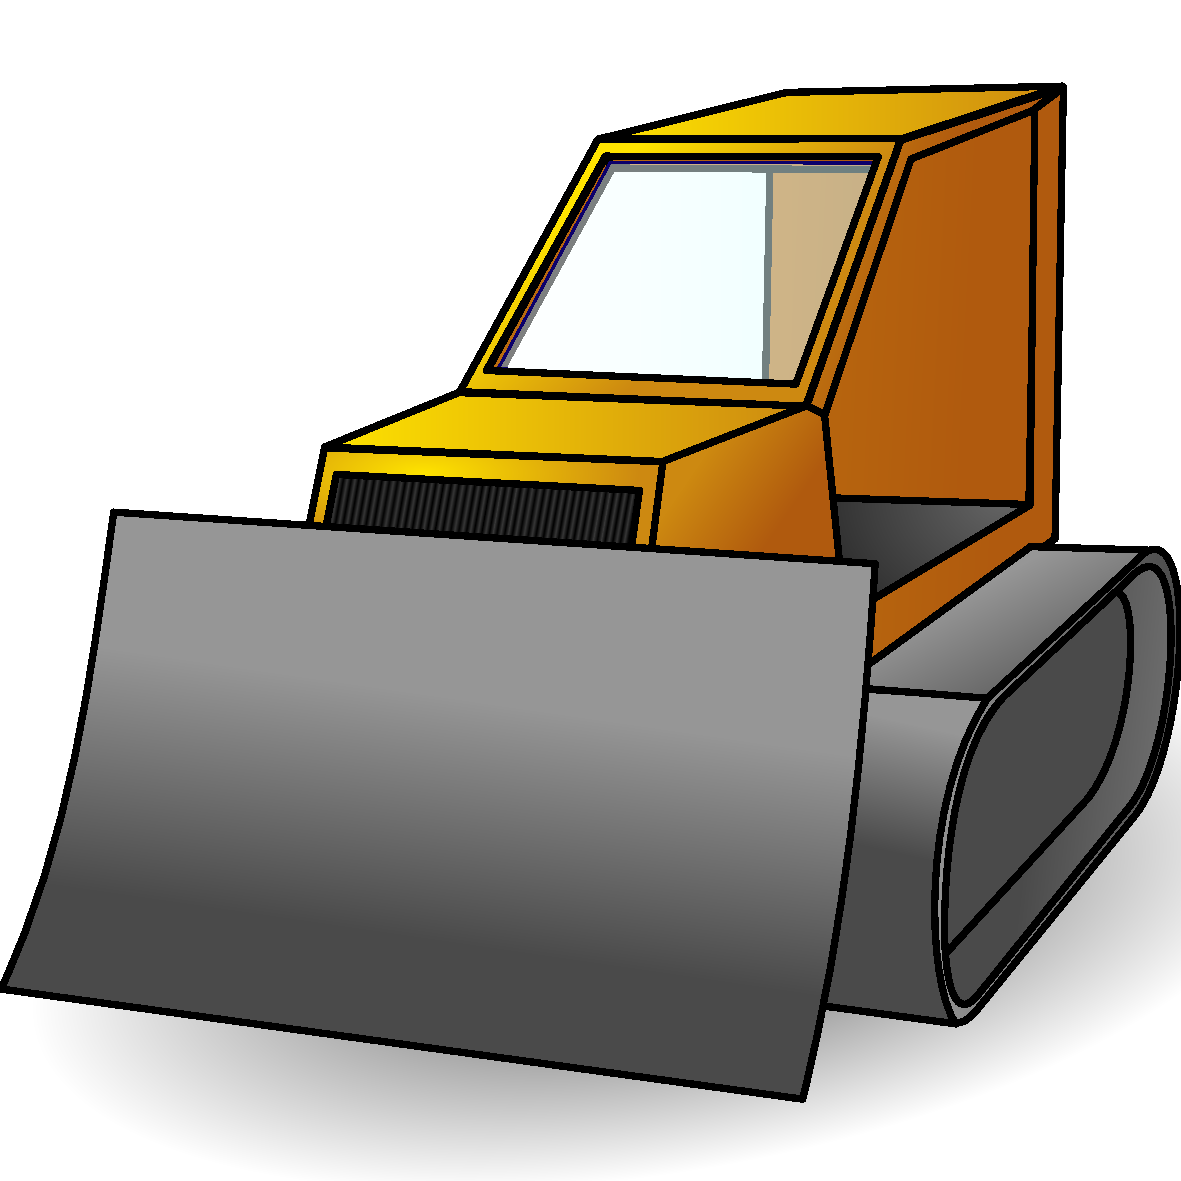
\includegraphics[width=.35\textwidth]{bulldozer}}
\end{floatrow}
\end{figure}

\sect{Steuerung des Roboter Thymio}

Der Roboter Thymio hat kein Steuerrad wie ein Auto und kein Lenker wie ein Fahrrad. Wie kann man ihn also lenken? Der Roboter benutzt ein \emph{Differentialgetriebe}, welches ähnlich funktioniert wie bei einem Raupenfahrzeug, z.B. einem Bulldozer (\cref{fig.bull}).
Die gewünschte Richtung wird mit Hilfe von \emph{unterschiedlichen} Geschwindigkeiten des linken und rechten Rades erreicht. Dreht das rechte Rad schneller als das linke, biegt das Fahrzeug nach links ab und dreht das linke Rad schneller als das rechte, biegt das Fahrzeug nach rechts ab.

In VPL wendet man das Differentialgetriebe an, indem man den linken und rechten Schieberegler des Motoraktionsblocks einzeln einstellt und dadurch die Geschwindigkeit der Räder verschieden einstellen kann.
Um einen möglichst grossen Unterschied der Geschwindigkeiten zu erreichen, lässt man die Räder in die entgegengesetzten Richtungen drehen. Tatsächlich dreht sich das Fahrzeug auf der Stelle, falls sich die Räder mit der genau \emph{gleichen} Geschwindigkeit in die entgegengesetzte Richtung bewegen.

Zum Beispiel wird im Aktionsblock \blksm{differential} der linke Regler auf schnelle Geschwindigkeit rückwärts und der rechte Regler auf schnelle Geschwindigkeit vorwärts eingestellt.  Als Resultat wird der Roboter eine enge Linkskurve vollführen, wie dies auf dem kleinen Bild des Roboter bzw. des Motoraktionsblocks dargestellt ist.

Experimentieren Sie mit einem Ereignis-Aktions-Paar wie diesem: \blkc{turning}

Stellen Sie den linken und rechten Schieber ein und lassen Sie das Programm laufen. Stoppen Sie dann den Roboter durch klicken auf \blksm{stop}. Ändern Sie nun die Schieberegler und versuchen Sie es erneut!

\trickbox{Das kleine Bild in der Mitte stellt den Thymio in seiner Bewegung dar. Wenn die Animation anhält, zeigt Thymio in die Richtung, in die sich der Roboter bewegen wird. }
	
\sect{Der Roboter mag Sie}

Ein echtes Haustier folgt seinem Meister. Damit der Roboter Ihrer Hand folgt,
muss man zwei weitere Ereignis-Aktions-Paare hinzufügen. Falls der Roboter ein Objekt vor seinem ganz links platzierten Distanzsensor wahrnimmt, soll er nach links drehen und falls er ein Objekt vor seinem ganz rechts platzierten Distanzsensor wahrnimmt, soll er nach rechts abbiegen.
                                                       
{\raggedleft \hfill Beispielprogramm \bu{likes.aesl}}

Das Programm für ''Der Roboter mag Sie'' besteht aus zwei Ereignis-Aktions-Paaren (\cref{fig.likes}).
Probieren Sie die Regler an jedem Motoraktionsblock aus!

\begin{figure}
	\subfigure[Der Roboter mag Sie]{
		\label{fig.likes}
		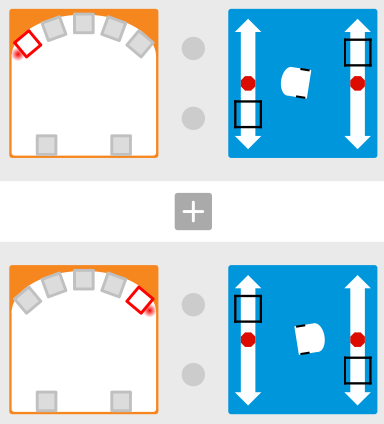
\includegraphics[width=.4\textwidth]{likes-turns}
	}
	\hfill
	\subfigure[Der Roboter mag Sie nicht]{
		\label{fig.hates}
		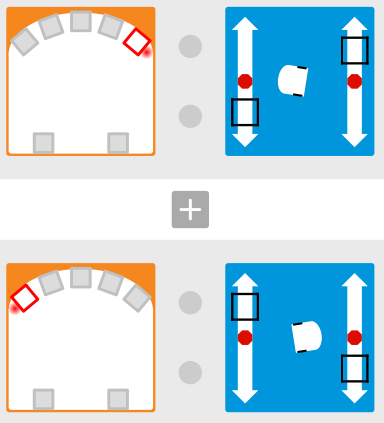
\includegraphics[width=.4\textwidth]{hates}
	}
	\caption{Programme für den Haustier-Roboter}\label{fig.likes-hates}
\end{figure}

\exercisebox{\thechapter.1}{Verändern Sie den Haustierroboter so, dass er vorwärts fährt, falls das Programm am laufen ist und stoppt, falls er das Ende des Tisches wahrnimmt.}

\exercisebox{\thechapter.2}{Was geschieht, wenn Sie die Reihenfolge der Ereignis-Aktions-Paare ändern?}

\sect{Der Roboter mag Sie nicht}

Manchmal mag dein Roboterhaustier in schlechter Laune sein und von deiner Hand zurückweichen. Erstellen Sie ein Programm, welches dieses Verhalten auslöst.

{\raggedleft \hfill Beispielprogramm \bu{does-not-like.aesl}}

Öffnen Sie das Programm für den Haustierroboter, der Sie mag und ändern Sie die Zusammenhänge zwischen Ereignissen und Aktionen. Das Erkennen eines Hindernisses beim linken Sensor bewirkt, dass der Roboter nach rechts abbiegt, 
während das Erkennen eines Hindernisses beim rechten Sensor bewirkt, 
dass der Roboter nach links abbiegt (\cref{fig.hates}).

% \begin{figure}[htb]
% \begin{center}
% \gr{hates}{0.4}
% \caption{The robot doesn't you}\label{fig.hates}
% \end{center}
% \end{figure}

\exercisebox{\thechapter.3} {Die vorderen horizontalen Sensoren sind von 0 bis 4 nummeriert (von links nach rechts). Die hinteren Sensoren tragen die Nummern 5 (links) und 6 (rechts). Ändern Sie das Programm \cref{fig.likes-hates} so dass anstelle der Sensoren 0 und 4...
\begin{itemize}[noitemsep,nosep,leftmargin=*]
\item die Sensoren 1 und 3 verwendet werden für die Drehung nach links bzw. rechts, 
\item die Sensoren 0 und 1 verwendet werden für die Linkskurve und die Sensoren 3 und 4 für die Rechtskurve.
\item Fügen Sie Ereignis-Aktions-Paare hinzu für die Sensoren 5 und 6.
\end{itemize}
}

\bigskip

\trickbox{\cref{a.tech} erklärt, wie man die Schieber für die Motorengeschwindigkeit präzise steuern kann.}

\informationbox{Sensoren im Fortgeschrittenen-Modus}{Im Fortgeschrittenen-Modus (siehe \cref{ch.time}), gibt es eine zusätzliche Art, um die Ereignisse abhängig von den Sensoren auszulösen (nachzulesen in  \cref{a.tech}).}

\chap{Thymio est sur une piste}\label{ch.line}

Considérez un entrepôt avec des charriots robotiques qui transportent des objets.
Il y a des lignes peintes sur le sol de l'entrepôt et le robot recoit comme instructions de suivre certaines lignes jusqu'à ce qu'il arrive à la zone de stockage de l'objet qu'il transporte.
Écrivons un programme qui permette à Thymio de suivre une ligne sur le sol.

{\raggedleft \hfill Programme: \bu{follow-line.aesl}}

Suivre une ligne sur le sol illustre le genre de difficultés rencontrées en robotique:
la ligne n'est pas forcément parfaitement droite,
de la poussière peut la recouvrir, ou de la saleté peut faire tourner une des roues du robot plus vite que l'autre.
Pour suivre une ligne malgré ces difficultés,
le robot doit utiliser un \emph{contrôleur}, qui aura pour tâche de définir la puissance à appliquer à chaque moteur en fonction des données reçues par les capteurs.

\sect{La ligne et le robot}

Pour suivre une ligne, nous allons utiliser les capteurs du sol que nous avons déjà utilisé dans le \cref{ch.moving}.
Rappelons qu'ils fonctionnent en envoyant de la lumière infrarouge (invisible pour l'oeil humain) et en mesurant la quantité de lumière renvoyée.
Si vous poser Thymio sur une couleur claire, beaucoup de lumière sera réfléchie, et donc l'événement \blksm{lots-of-light} sera déclenché.
Nous avons donc besoin d'une ligne qui déclenchera un événement quand peu de lumière sera réfléchie \blksm{little-light}.
Ceci est facile à réaliser en imprimant une bande noire, en la peignant ou en utilisant du ruban adhésif noir comme sur la \cref{fig.tape}.
La ligne doit être assez large pour que les deux capteurs de sol voient du noir quand le robot suit la ligne correctement.
Une largeur de 5 centimètres est suffisante pour que le robot suive la ligne même s'il dévie un peu.

\begin{figure}
    \subfigure[Thymio suit une ligne]
        {\label{fig.tape}
        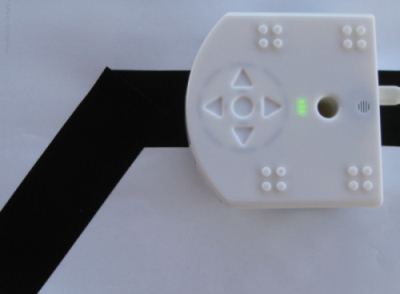
\includegraphics[height=0.35\textwidth]{blacktape}}
    \hfill
    \subfigure[Le capteur gauche est hors de la ligne,
    le capteur droite est sur la ligne. Le point rouge
    indique que le capteur gauche mesure beaucoup de lumière
    réfléchie]{
        \label{fig.one-off}
        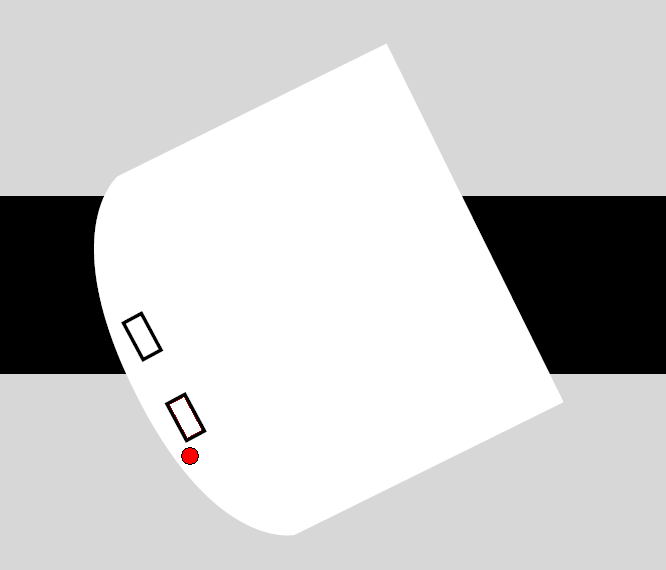
\includegraphics[height=0.35\textwidth]
        {thymio_half_on_line}}
    \caption{Thymio sur une ligne de ruban adhésif noir}
\end{figure}


Le premier pas pour faire suivre une ligne à Thymio est de le faire avancer s'il est sur la ligne (les \emph{deux} capteurs de sol détectent du foncé), et de le faire s'arrêter s'il ne se trouve pas sur la ligne (les \emph{deux} capteurs de sol détectent du clair).
Voir \cref{fig.start-stop}.

\begin{figure}
	\subfigure[Thymio s'arrête ou avance]{ \label{fig.start-stop} 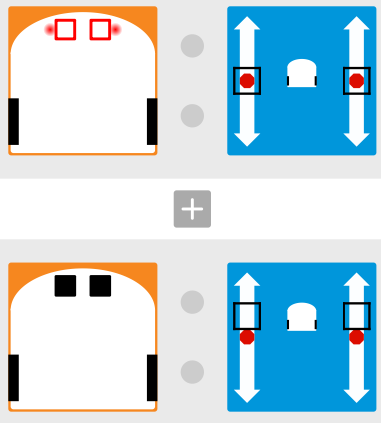
\includegraphics[width=0.4\textwidth]{line-forward}}
	\hfill
	\subfigure[Thymio corrige les déviations]{ \label{fig.follow-line} 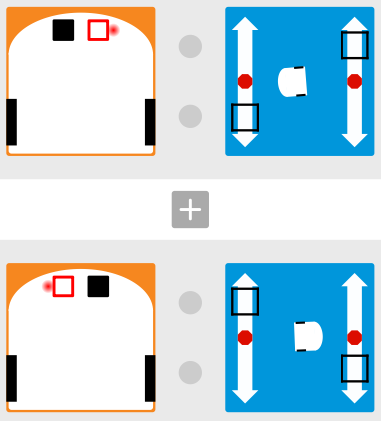
\includegraphics[width=0.4\textwidth]{line-controller}}
	\caption{Un programme pour suivre une ligne}
        \label{fig.follow-line-all}
\end{figure}

\trickbox{Assurez-vous d'avoir un câble USB assez long (disons, deux mètres) pour que le robot reste connecté même quand il bouge.
Vous trouverez des rallonges dans les magasins d'informatique.}

\sect{Votre premier contrôleur}

Le prochain pas consiste à programmer le contrôleur qui suit la ligne.
Deux paires événement-actions sont nécessaires (\cref{fig.follow-line}).

\begin{itemize}
    \item Si le robot sort de la ligne à \emph{gauche}
    \cref{fig.one-off}), le capteur \emph{gauche}
    détectera le sol alors que le capteur \emph{droite}
    continuera de détecter la ligne ;
    dans ce cas le robot doit tourner légèrement à
    \emph{droite}.

    \item Si le robot sort de la ligne à \emph{droite},
    le capteur \emph{droite} détectera le sol
    alors que le capteur \emph{gauche} continuera
    de détecter la ligne ; dans ce cas le robot
    doit tourner légèrement à \emph{gauche}.
	
\end{itemize}

\sect{Régler les paramètres}

Il est assez facile de comprendre que
si Thymio sort de la ligne à gauche,
il doit tourner à droite (\cref{fig.one-off}).
La question est plutôt: de combien doit-il tourner ?
Si la rotation est trop douce, le capteur droit pourrait aussi sortir de la ligne avant que le robot ne tourne assez ;
si au contraire le tour est trop serré, le robot pourrait sortir de la ligne de l'autre côté.
Dans tous les cas, des tours trop forts peuvent être dangereux pour le robot et ce qu'il transporte et qui risque de tomber.

Vous devrez expérimenter avec la vitesse des roues gauche et droite dans chaque bloc action moteurs
jusqu'à ce que le robot bouge de manière \emph{fiable}.
Par fiable, nous entendons que le robot peut réussir plusieurs fois l'expérience de suivi de ligne.
Comme à chaque expérience vous placez le robot sur la ligne à différentes positions et pointant dans differentes directions, il faut tester plusieurs fois pour être convaincu que le programme fonctionne.

Thymio doit-il aller vite lorsqu'il est sur la ligne ou, au contraire, lentement ?
En allant vite, vous améliorerez son efficacité pour se déplacer d'un point à un autre mais il risquera de sortir de la ligne avant de pouvoir corriger sa direction.
À l'inverse, s'il va trop lentement, personne n'achètera votre robot pour l'utiliser dans en entrepôt.
%De plus, une fois que Thymio remarque qu'il quitte la ligne, que doit-il faire ?
%S'il fait tourner un moteur dans un sens et l'autre dans le sens oppposé, vous vous assurez qu'il ne quittera pas la ligne mais ses mouvements seront très saccadés.
%S'il corrige simplement sa trajectoire en diminuant la vitesse d'une roue, il se déplacera avec fluidité, mais il risquera de quitter complètement la ligne.
%Ainsi, il faudra trouver de bons compromis.

\exercisebox{\thechapter.1}{
Thymio s'arrête complètement s'il ne détecte plus du tout la ligne.
Modifiez le programme pour qu'il tourne lentement sur lui même vers la gauche jusqu'à ce qu'il retrouve la ligne.
Essayez le sur une ligne avec un virage à gauche comme sur la \cref{fig.tape}.
Essayer d'augmenter la vitesse en avant du robot.
Que se passe-t-il lorsque le robot arrive à la fin de la ligne ?
}

\bigskip

\exercisebox{\thechapter.2}{
Modifiez le programme de l'exercice précédent pour que le robot tourne à droite quand il arrive au bout de la ligne.
Que se passe-t-il ?
\vspace{.5em}\\
Il serait bien de pouvoir se \emph{rappeller} quel capteur était le dernier à perdre le contact avec la ligne afin de faire tourner le robot dans la bonne direction pour retrouver la ligne.
Dans le \cref{ch.states}, nous apprendrons à Thymio à se rappeler ces informations.
}

\bigskip 

\exercisebox{\thechapter.3}{
Jouez avec différentes formes de parcours :
\begin{itemize}[noitemsep,nosep,leftmargin=*]
\item Des virages doux
\item Des virages serrés
\item Des zig-zag
\item Des lignes plus larges
\item Des lignes plus étroites
\end{itemize}
Faites la course avec vos amis :
Quel robot suit le plus de lignes différentes avec succès ?
Pour chaque ligne, quel robot la suit dans le moins de temps ?
}

\bigskip

\exercisebox{\thechapter.4}{
Discutez les effets que les modifications suivantes au Thymio auraient sur les capacités du robot à suivre une ligne :
\begin{itemize}[noitemsep,nosep,leftmargin=*]
\item L'événement de lecture des capteurs de sol devient plus ou moins fréquent.
\item Les capteurs sont plus éloignés ou proche l'un de l'autre.
\item Il y a plus que deux capteurs de sol sous le robot.
\end{itemize}
}

% TODO

% !TeX root = vpl.tex

\chap{Sonagli e fischietti}\label{ch.bells}

Prendiamoci qualche momento di svago dai compiti complessi come seguire una linea e
divertiamoci un po' con il nostro robot Thymio.
In questo capitolo ti mostriamo come il Thymio possa riprodurre musica, rispondere a un suono o reagire quando viene toccato.

\sect{Suonare musica}

Il robot Thymio contiene un sintetizzatore di suoni e si può programmare
per riprodurre melodie semplici utilizzando il blocco di azione musica: \blkc{action-music}

{\raggedleft \hfill File di programma \bu{bells.aesl}}

Non diventerai un nuovo Beethoven---si può suonare solo una sequenza di note alla volta,
su cinque toni e due lunghezze differenti---ma si può comporre una
melodia che farà distinguere il vostro robot da tutti gli altri. La \Cref{fig.music} mostra
due coppie evento-azione che rispondono con una melodia quando il pulsante anteriore o posteriore
vengono toccati. C'è una melodia diversa associato ad ogni evento.

\begin{figure}
\begin{center}
\gr{music}{.4}
\caption{Esegui una melodia}\label{fig.music}
\end{center}
\end{figure}

Il piccoli cerchi sono le sei note.
Una nota nera è una nota breve e una nota bianca è una nota lunga; per passare da una lunghezza all'altra, cliccare sul cerchio.
Ci sono cinque righi orizzontali colorati, che rappresentano cinque toni.
Per spostare un cerchio su un rigo, fare clic sul \emph{rigo} sopra o sotto il cerchio.
Non cercare di trascinare e rilasciare una nota; non funzionerà.

\exercisebox{\thechapter.1}{
Scrivere un programma che vi permetterà di inviare un messaggio in \href{http://en.wikipedia.org/wiki/Morse_code}{codice Morse}.
Le lettere in codice Morse sono codificate in sequenze di toni lunghi
(\emph{linee}) e toni brevi (\emph{punti}). Ad esempio, la lettera
\emph{V} è codificato da tre punti seguiti da una linea.}


\sect{Controllare il tuo robot con i suoni}

Il Thymio ha un microfono. L'evento \blksm{event-clap} si verificherà
quando il microfono avverte un forte rumore, per esempio un applauso con le tue
mani. la seguente coppia evento-azione accende le luci della parte inferiore
quando battete le mani: \blkc{clap}

\trickbox[Informazioni] {In un ambiente rumoroso potresti non essere in grado di utilizzare questo
evento, perché il livello sonoro sarà sempre alto causando ripetuti
eventi.}

\exercisebox{\thechapter.2}{
Scrivi un programma che fa muovere il robot quando batti
le mani e lo fa fermare quando si tocca un tasto.
\vspace{.5em}\\
Quindi scrivi un programma che fa il contrario: si avvia quando si tocca un tasto
e si ferma quando batti le mani.
}


\sect{Ottimo lavoro, robot!}

Gli animali non sempre fanno quello che chiediamo loro di fare. A volte hanno bisogno di una pacca
sulla testa per incoraggiarli. Si può fare lo stesso con il vostro robot. Il
Thymio contiene un sensore di urto che provoca l'evento \blksm{event-tap} in risposta ad un rapido tocco sulla parte superiore del robot. Per esempio,
la seguente coppia evento-azione fa sì che le luci superiori si accendano quando
si tocca la parte superiore del robot: \blkc{touch}

Costruisci un programma da questa coppia evento-azione e la seguente coppia
che accende le luci inferiori quando batti le mani: \blkc{clap}

{\raggedleft \hfill File di programma {bu whistles.aesl}}

Riesci ad attivare solo la parte superiore delle luci? Questo è difficile da fare: un colpetto
provoca un suono che può essere abbastanza forte da far accendere pure le luci inferiori. Con un po' di pratica sono riuscito a toccare il robot
abbastanza delicatamente in modo che il suono emesso dal colpetto non è stato considerato un evento.

\exercisebox{\thechapter.3}{
Scrivere un programma che faccia andare avanti il robot fino a quando non colpisce una
parete.
\vspace{.5em}  \\
\textbf{Assicurarsi} che il robot si \textbf{muova lentamente} in modo che
non si danneggi.
}


\chap{Angenehme Zeit (Fortgeschrittener Modus)}\label{ch.time}

Im \cref{ch.pet} haben wir ein Roboterhaustier programmiert, das uns entweder mag oder nicht mag. Nun stellen wir uns ein etwas komplizierteres Verhalten vor: ein schüchternes Haustier, welches sich nicht entscheiden kann, ob es uns mag oder nicht. Anfänglich wird das Haustier sich unserer Hand zuwenden, dann aber zurückweichen und schlussendlich sich wieder zu unserer Hand hinbewegen.

{\raggedleft \hfill Beispielprogramm \bu{shy.aesl}}

Das Verhalten des Roboters ist wie folgt: Falls der Rechte Schalter berührt wird, bewegt sich der Roboter nach rechts, falls er Ihre Hand wahrnimmt, bewegt er sich nach links, aber nach einer Weile bereut er die Entscheidung und bewegt sich wieder zurück. Wir wissen, wie wir die Ereignis-Aktions-Paare für die erste Bewegung erstellen:
\blkc{start-turn} 
und wie für das zurück-bewegen, falls Ihre Hand erkannt wird:
\blkc{turn-away}
Das Verhalten des Zurückweichens ``nach einer Weile'' kann in zwei Ereignis-Aktions-Paare zerlegt werden:

\begin{itemize}

\item \emph{Falls} der Roboter sich wegbewegt $\rightarrow$
\emph{starte einen Timer} für zwei Sekunden.

\item \emph{Falls} der Timer null erreicht $\rightarrow$ \emph{drehe}
nach rechts ab.

\end{itemize}

Wir brauchen eine neue \emph{Aktion} für das erste Verhalten und ein neues \emph{Ereignis} für das zweite Verhalten.

Die Aktion ist, einen \emph{Timer} einzustellen, welcher wie ein Wecker funktioniert \blksm{action-timer}.  Normalerweise stellen wir den Wecker auf eine bestimmte Zeit ein, aber falls ich den Wecker auf meinem Smartphone auf eine bestimmte Zeit einstelle, wird mir diese als Zeitdauer angegeben: ``Wecker läutet in 11 Stunden und 23 Minuten''. Der Timerblock arbeitet auf die selbe Art und Weise. Der Timer wird auf eine bestimmte Anzahl Sekunden eingestellt, sobald das Ereignis stattfindet und die Aktion ausgelöst wird. Der Timer kann auf bis zu vier Sekunden eingestellt werden. Klicken Sie irgendwo innerhalb des schwarzen Kreises, wo die Oberfläche der Uhr gezeigt wird (aber nicht auf den schwarzen Kreis selber). Nach einer kleinen Animation wir die Zeitdauer des Timers (bis der Alarm ausgelöst wird) in blauer Farbe angezeigt.

Das Ereignis-Aktions Paar für das erste, oben beschriebene Verhalten ist: \blkc{turn-clock}

Der Timer ist auf zwei Sekunden eingestellt. Falls das Ereignis Handerkennung stattfindet, werden zwei Aktionen ausgelöst: Drehung des Roboters nach links und Starten des Timers.

Der zweite Teil dieses Verhaltens benötigt ein Ereignis, das stattfindet, falls der Alarm ausgelöst wird. Dieses tritt ein, sobald die eingestellte Zeit abgelaufen ist. Der Ereignisblock \blksm{event-timer} zeigt dann einen klingelnden Wecker.

\informationbox{Fortgeschrittener Modus}{Timer werden nur im \emph{Fortgeschrittenen Modus} unterstützt. Klicken Sie auf \blkmed{advanced} um in den fortgeschrittenen Modus zu gelangen.\\Das Icon ändert in \blkmed{basic}; durch erneutes Klicken gelangt man zurück in den \emph{Standard-Modus}.}

Das Ereignis-Aktions-Paar ist: \blkc{turn-back} welches den Roboter zurück nach rechts drehen lässt, sobald der Timer abgelaufen ist.

\exercisebox{\thechapter.1}{
	Schreiben Sie ein Programm, welches den Roboter bei Höchstgeschwindigkeit für drei Sekunden vorwärts fahren und danach wieder zurückkehren lässt, sobald der Vorwärtsschalter gedrückt wird. Fügen Sie ein Ereignis-Aktions-Paar hinzu, das die Fahrt des Roboters stoppt, falls der mittlere Schalter gedrückt wird.}

\chap{Les états (Mode avancé)}\label{ch.states}

Un programme VPL est composé d'une série de paires événement-actions.
\emph{Tous} les événements sont vérifiés périodiquement et les actions appropriées sont effectuées.
Ceci limite les programmes que nous pouvons créer ; pour aller plus loin nous avons besoin d'une façon de spécifier que certaines paires événement-actions sont actives à un certain moment, alors que d'autres ne le sont pas.

Par exemple, quand Thymio devait suivre une ligne (\cref{ch.line}), lorsque le robot sortait de la ligne, nous aurions aimé qu'il tourne à gauche ou à droite afin de rechercher la ligne dans une direction qui dépendait de quel côté il était sorti.
Pour cela, deux paires événement-actions sont nécessaires:
une pour tourner à gauche lorsque le robot sort à droite de la ligne
et une pour tourner à droite lorsqu'il sort à gauche.

%Les états sont disponibles dans le mode \emph{avancé} de VPL.
%Cliquez sur \blksm{advanced} avant de travailler sur les projets de ce chapitre.

\sect{Tape, tape}

Dans les programmes que nous avons réalisé jusqu'ici, nous avons souvent \emph{démarré} Thymio en appuyant sur un de ces boutons et \emph{arrêté} Thymio en appuyant sur un autre.
Mais regardez votre ordinateur, normalement, il n'a qu'un seul bouton pour l'allumer ou l'éteindre.
%\blksm{power-button} 
Le bouton se \emph{rappelle} s'il est dans l'état \bu{allumé} ou l'état \bu{éteint}.

Écrivons un programme qui allume les lumières du robot si vous lui donnez une petite tape et qui les éteigne si vous lui donnez une seconde tape.

{\raggedleft \hfill Programme \bu{tap-on-off.aesl}}

Il est pratique de décrire ce comportement en utilisant un \textit{diagramme d'états} :

\begin{center}
\begin{picture}(240,45)
\thicklines
%\put(0,0){\framebox(240,40){}}
\put(20,20){\circle{40}}
\put(0,0){\makebox(40,40){\textsf{éteint}}}
\put(220,20){\circle{40}}
\put(200,0){\makebox(40,40){\textsf{allumé}}}
\put(40,30){\vector(1,0){160}}
\put(0,30){\makebox(240,10){\textsf{tape $\rightarrow$ allumer}}}
\put(200,10){\vector(-1,0){160}}
\put(0,10){\makebox(240,10){\textsf{tape $\rightarrow$ éteindre}}}
\end{picture}
\end{center}

Ce diagramme comprend deux états indiqués par des cercles, \bu{allumé} et \bu{éteint}.
Depuis l'état \bu{éteint}, le robot peut aller dans l'état \bu{allumé} et revenir, mais seulement en suivant les instructions sur les flèches.
Les instructions décrivent quand une transition d'un état à l'autre peut se produire et comment :

\begin{itemize}

\item \emph{Quand} Thymio est dans l'état \bu{éteint} \textbf{\textit{et}} que l'événement \emph{tape} se produit $\rightarrow$ \emph{allumer} le robot \textbf{\textit{et}} aller dans l'etat \bu{allumé}.

\item \emph{Quand} Thymio est dans l'état \bu{allumé} \textbf{\textit{et}} que l'événement \emph{tape} se produit $\rightarrow$ \emph{éteindre} le robot \textbf{\textit{et}} aller dans l'etat \bu{éteint}.

\end{itemize}

L'accent mis sur le mot \textbf{\textit{et}} avant la flèche~$\rightarrow$ signifie que deux conditions doivent être remplies pour que la transition se fasse: (a) le robot doit être dans un certain état et (b) l'événement doit se produire.
Lorsque les deux conditions sont remplies, alors la transition est prise ce qui fait à la fois changer l'état et exécute l'action écrite après la flèche~$\rightarrow$.

Il est important de réaliser que les deux parties de la condition sont indépendantes.
Dans le diagramme ci-dessus (répété ici),
l'événement \emph{tape} apparaît deux fois, mais l'action 
exécutée lorsque cet événement a lieu 
\emph{dépend de l'état du robot}.

\vspace*{-1ex}

\begin{center}
\begin{picture}(240,40)
\thicklines
%\put(0,0){\framebox(240,40){}}
\put(20,20){\circle{40}}
\put(0,0){\makebox(40,40){\textsf{éteint}}}
\put(220,20){\circle{40}}
\put(200,0){\makebox(40,40){\textsf{allumé}}}
\put(40,30){\vector(1,0){160}}
\put(0,30){\makebox(240,10){\textsf{tape $\rightarrow$ allumer}}}
\put(200,10){\vector(-1,0){160}}
\put(0,10){\makebox(240,10){\textsf{tape $\rightarrow$ éteindre}}}
\end{picture}
\end{center}

\vspace*{-1ex}

Dans un même état, différents événements peuvent causer différentes actions et des transitions vers de nouveaux états différents.
Dans le diagramme suivant, toucher le bouton de gauche
dans l'état \textbf{éteint} allume la lumière verte du robot
et passe l'état du robot à \textbf{allumé1},
alors que toucher le bouton droit \textbf{dans le même état}
entraîne une autre action, allumer la lumière rouge,
et un autre changement d'état vers \textbf{allumé2}.

\vspace*{-1ex}

\begin{center}
\begin{picture}(300,80)
\thicklines
%\put(0,0){\framebox(240,80){}}
\put(25,42){\circle{40}}
\put(10,28){\makebox(30,30){\textsf{éteint}}}
\put(280,20){\circle{40}}
\put(265,6){\makebox(30,30){\textsf{allumé2}}}
\put(40,57){\vector(1,0){220}}
\put(280,65){\circle{40}}
\put(265,50){\makebox(30,30){\textsf{allumé1}}}
\put(40,27){\vector(1,0){220}}
\put(0,60){\makebox(295,10){\textsf{bouton gauche $\rightarrow$ s'allumer en vert}}}
\put(0,30){\makebox(295,10){\textsf{bouton droite $\rightarrow$ s'allumer en rouge}}}
\end{picture}
\end{center}

\sect{Implémenter des diagrammes d'états avec des paires événement-actions}

Nous montrons comment \emph{implémenter} le comportement décrit par le diagramme d'état avec des paires événement-actions.
Implémenter signifie construire un programme qui fera ce que le diagramme d'états ci-dessus décrit.
La \cref{fig.turn-on-off} montre le programme.
Regardons maintenant les paires événement-actions une à une.
Le cercle gauche du bloc \blksm{event-tap-advanced} est
sélectionné (et s'affiche en rouge) pour indiquer qu'il s'agit d'un bloc pour l'événement tape.

\importantbox[Le bloc tape en mode avancé]{
Le bloc pour l'événement tape est différent en mode avancé
car il permet aussi l'utilistation des événements
accéléromètre comme décrit au \cref{ch.angles}.}

\begin{figure}
    \subfigure[Une tape pour allumer la lumière]{
        \label{fig.turn-on-off1}
        
\includegraphics[width=.6\textwidth]{tap-on-off1}
    }
    \subfigure[Une tape pour éteindre la lumière]{
        \label{fig.turn-on-off2}
        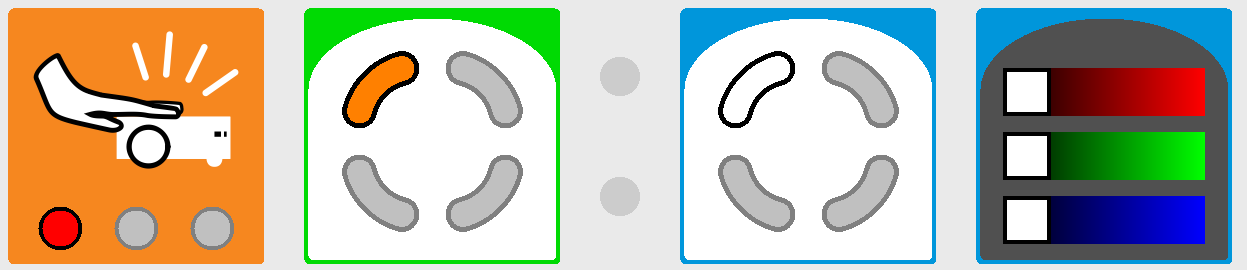
\includegraphics[width=.6\textwidth]{tap-on-off2}
    }
    \caption{Une tape qui a des résultats différents en fonction de l'état.}
    \label{fig.turn-on-off}
\end{figure}

Dans la première paire événement-actions (\cref{fig.turn-on-off1}), l'événement est composé du bloc événement tape avec une indication d'état \blksm{state-filter}.
Un état est indiqué par quatre quartiers d'un cercle, chacun pouvant être soit allumé (orange) ou éteint (blanc).
Dans ce programme, nous utiliserons le quartier en haut à gauche pour indiquer si la lumière du haut du robot est éteinte ou allumée.
Dans \cref{fig.turn-on-off1}, ce quartier est coloré en blanc
et donc la lumière du robot est éteinte.
Ainsi, cette paire veut dire : \textbf{si} le robot est tapé \textbf{et} que le robot est éteint, \textbf{alors} allumer la lumière du robot.

Dans la seconde paire événement-actions
(\cref{fig.turn-on-off2}),
le quartier est coloré en orange et donc la lumière du robot est allumée.
Cette paire veut dire : \textbf{si} le robot est tapé \textbf{et} qu'il est allumé, \textbf{alors} l'éteindre.

Si vous regardez à nouveau le diagramme d'états, vous verrez que seulement la moitié du travail est fait.
En effet, en allumant et éteignant le robot, nous devons aussi changer son état d'\bu{éteint} à \bu{allumé} ou d'\bu{allumé} à \bu{éteint}.
Ainsi, il nous faut ajouter un bloc action \emph{état} \blksm{action-states} à chaque paire.
Ce bloc change l'état selon si les quartiers sont blancs ou oranges.

Pour résumer, la signification du programme de la figure \cref{fig.turn-on-off} est la suivante :

\begin{quote}
    \emph{Quand} le robot est tapé \emph{et} que l'état est \emph{éteint},\\ changer l'état à \bu{allumé} \emph{et} \bu{allumer} la lumière du haut.\\
    \emph{Quand} le robot est tapé \emph{et} que l'état est \bu{allumé},\\changer l'état à \bu{éteint}
    \emph{et} \bu{éteindre} la lumière du haut.
\end{quote}

Chaque événement entraîne à la fois une action lumière et une action état.
Les actions dépendent de l'état dans lequel le robot se trouve, appellé \emph{état actuel}.

\sect{Dans combien d'états différents Thymio peut-il être?}

Quand il est utilisé avec un bloc événement état ou action état, chaque quartier peut être :
\begin{itemize}
	\item \textbf{Blanc}: le quartier est \emph{éteint} ;
	\item \textbf{Orange}: le quartier est \emph{allumé} ;
	\item \textbf{Gris}: le quartier n'est pas pris en compte.
\end{itemize}

Par exemple, dans \blksm{states}, les quartiers en haut à gauche et en bas à droite sont allumés, le quartier en haut à droite est éteint, et le quartier en bas à gauche n'est pas pris en compte.
Ceci veut dire que si \blksmpure{states} est associé à un bloc événement, l'événement se produira si l'état est défini soit par :
\begin{center}
\centering \makebox{\raisebox{-1.7em}{
\includegraphics[height=4em]{states1}}}\quad ou \quad \makebox{\raisebox{-1.7em}{
\includegraphics[height=4em]{states2}}}
\end{center}

Comme chacun des quatre quartiers peut être soit allumé soit éteint, il y a 2 $\times$ 2 $\times$ 2 $\times$ 2 = 16 états :
\begin{quote}
\bu{(éteint, éteint, éteint, éteint)\\(éteint, éteint, éteint, allumé)\\(éteint, éteint, allumé, éteint)\\
\mbox{}\hspace{3em}\ldots\\
(allumé, allumé, allumé, éteint)\\
(allumé, allumé, allumé, allumé)}.
\end{quote}
La \cref{fig.all-states} montre tous les états possibles.
\importantbox{L'état courant du robot est toujours affiché sur le haut du robot par les quatre arcs de cercles lumineux.
Par exemple, la \cref{fig.state-leds} montre le robot dans l'état \bu{(allumé, allumé, allumé, allumé)}.}

\trickbox[Information]{Lorsqu'un programme démarre, l'état initial est toujours 
\bu{(éteint, éteint, éteint, éteint)}:\quad \blkmed{state-all-off}}

\trickbox{Si vous n'utilisez pas tous les 16 états possibles, mais par exemple que 2 ou 4, vous êtes libre de décider quel quartier vous utiliser pour représenter votre état.
Aussi, si par exemple vous avez deux choses différentes à encoder dans l'état, et que chacune d'elle a deux valeurs possibles, vous pouvez utiliser deux quartiers indépendemment.
C'est pourquoi la capacité d'\emph{ignorer} un quartier est très utile !
Essayez toujours de rester le plus simple possible.
}

\begin{figure}
	\subfigure[Tous les états possibles de Thymio]{
		\label{fig.all-states}
		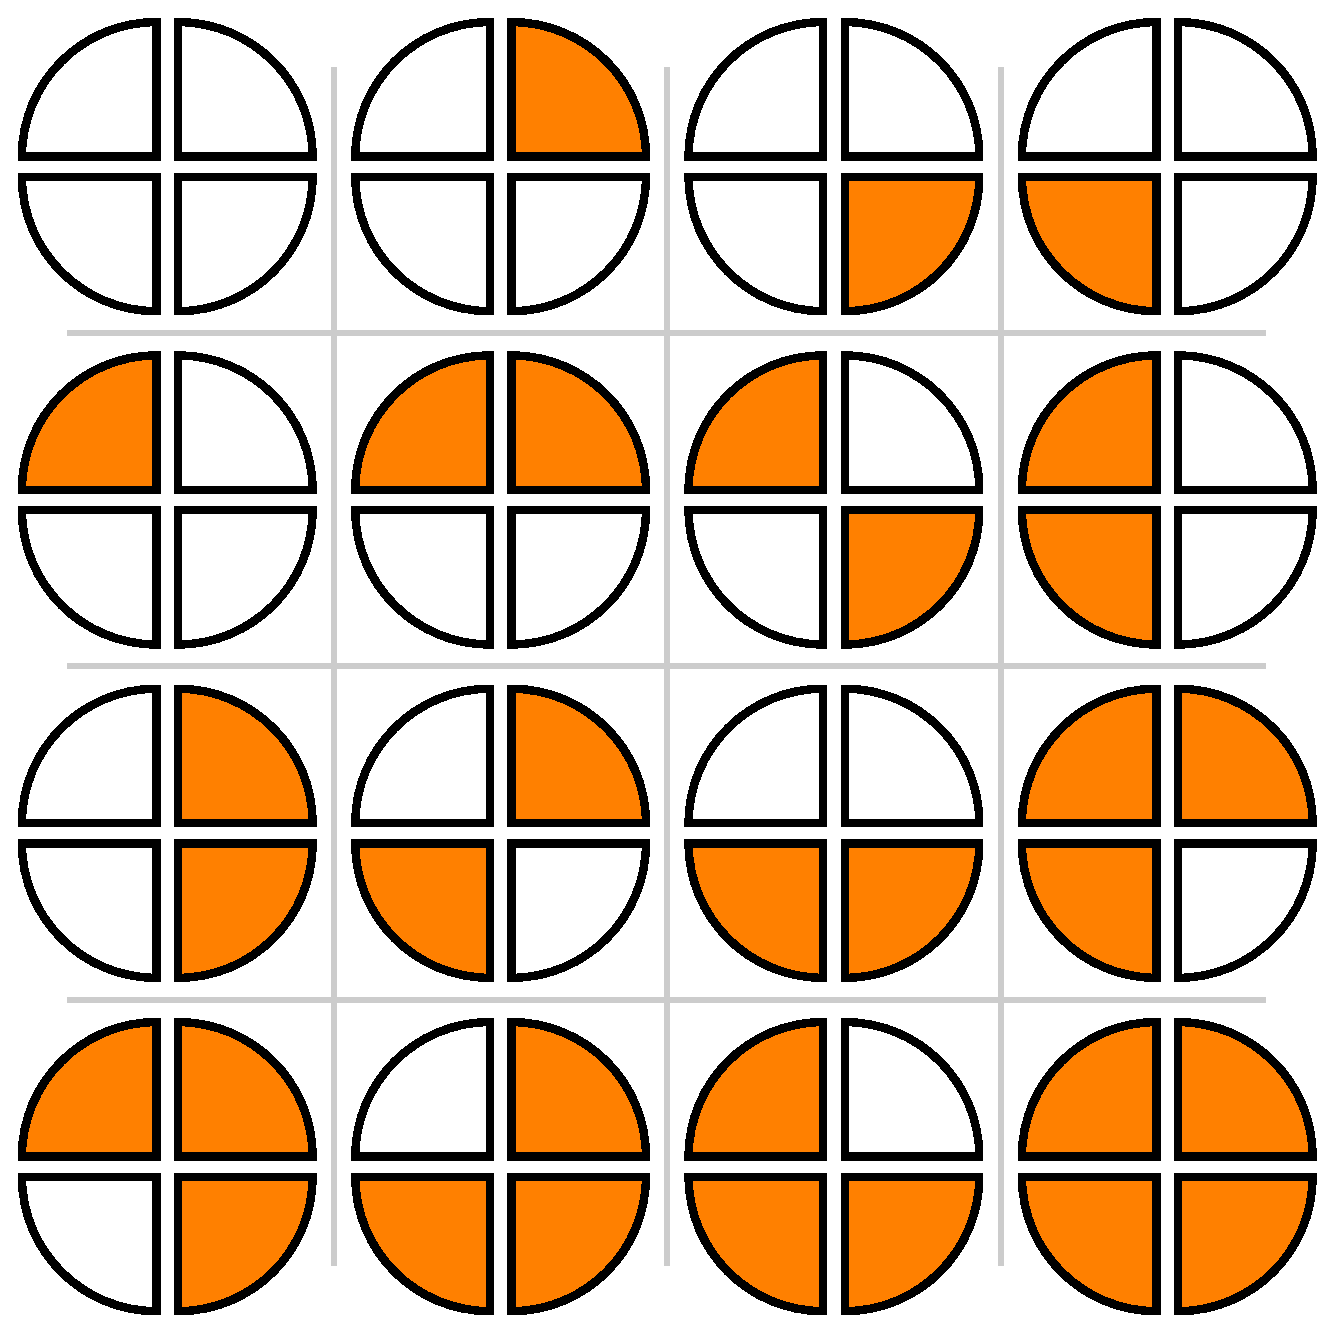
\includegraphics[width = 0.4\textwidth]{all-states}
	} 
	\hfill
        \subfigure[La cercle de lumières indique l'état]{
		\label{fig.state-leds}
		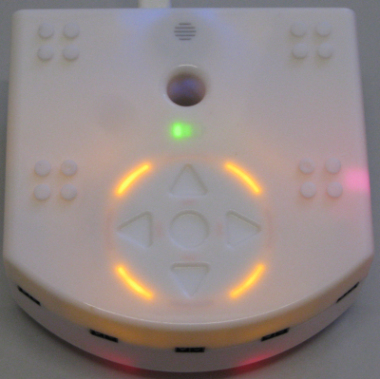
\includegraphics[width = 0.4\textwidth]{state-leds}
	}
	\caption{Les états de Thymio et leur représentation}
\end{figure}

\sect{Attraper la souris}

Écrivons un programme qui fasse tourner le robot de droite à gauche à la recherche d'une souris (ou d'un autre objet).
Si le robot détecte une souris avec son capteur tout à gauche, il continue la recherche jusqu'à ce que la souris soit détectée avec son capteur tout à droite.
Puis, il se positionne en face de la souris, comme sur la \cref{fig.cat-mouse}.

{\raggedleft \hfill Programme: \bu{mouse.aesl}}

Le diagramme d'état suivant décrit le comportement du robot:

\begin{center}
\unitlength=1.2pt
\begin{picture}(320,35)
    %\put(0,0){\framebox(320,35){}}
    \put(40,10){\oval(80,20)}
    \put(160,10){\oval(80,20)}
    \put(280,10){\oval(80,20)}
    \put(0,0){\makebox(80,20){\bu{chercher à gauche}}}
    \put(120,0){\makebox(80,20){\bu{chercher à droite}}}
    \put(240,0){\makebox(80,20){\bu{trouvé}}}
    \put( 80,10){\vector(1,0){40}}
    \put(200,10){\vector(1,0){40}}
    \put(40,35){\vector(0,-1){15}}
\end{picture}
\end{center}

\begin{enumerate}
\item Lorsque le bouton central est touché, le robot entre dans l'état \bu{chercher à gauche} et 
    tourne de droite à gauche.
\item Lorsque le robot est dans l'état \bu{chercher à gauche}
    et détecte la souris sur son capteur tout à droite,
    il prend l'état \bu{chercher à droite} et tourne de gauche à droite.
\item Lorsque le robot est dans l'état \bu{chercher à droite}
    et il détecte la souris avec son capteur central,
    il prend l'état \bu{trouvé} et s'arrête.
\end{enumerate}

L'essentiel est de remarquer que lorsque le capteur central détecte la souris,
le robot s'arrête \emph{seulement si} le robot est dans l'état \bu{chercher à droite}.
Sinon (si la souris est détectée par le capteur central en mode \bu{chercher à gauche}), rien ne se produit.

\begin{figure}
    \begin{center}
        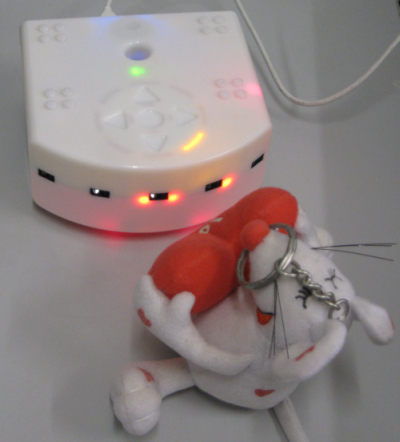
\includegraphics[width=0.4\textwidth]{cat-mouse}
	\caption{Le robot chat cherche la souris}
        \label{fig.cat-mouse}
    \end{center}
\end{figure}

Implémentons ce comportement.
L'état du robot sera défini par le quartier supérieur gauche.
Choisissons le blanc pour représenter l'état \bu{chercher à gauche} et l'orange pour représenter l'état \bu{chercher à droite}.
Puisque le programme se termine lorsque la souris est détectée dans l'état \bu{chercher à droite},
nous n'avons pas besoin de représenter l'état final \bu{trouvé}.
Initialement, tous les quartiers sont \bu{éteints} (blancs).

La paire événement-actions suivante fait tourner le robot à gauche : \blkc{mouse1}
Quand le bouton central est touché, l'état change et devient
\bu{chercher à gauche} \emph{et} le robot tourne à gauche.

%Ceci se produira lorsque le quartier gauche-haut est éteint ; initialement tous les quartiers de l'état sont éteint.

La prochaine paire événement-actions implémente la deuxième étape: \blkc{mouse2}
Quand le robot est dans l'état \bu{chercher à gauche} et
que la souris est détectée par le capteur tout à droite,
l'état devient \bu{chercher à droite}
\emph{et} le robot tourne vers la droite.

Notez que le petit carré à côté de ce capteur est noir pour que l'événement se produise seulement si seul le capteur le plus à droite détecte la souris.

La troisième étape est implémentée dans la paire événement-actions suivante: \blkc{mouse3}
Lorsque la souris est détectée par le capteur central dans l'état \bu{chercher à droite}, le robot s'arrête.


%Pourquoi l'événement de cette paire doit-il dépendre de l'état ?
%La raison est que le capteur central détectera aussi la souris durant le scan initial de droite à gauche.
%Nous voulons que le robot fasse d'abord un scan complet avant de retourner à la position de la souris ; il est donc nécessaire que cette première détection soit ignorée.
%Ceci est accomplit en arrêtant le scan seulement lorsque l'état est \bu{allumé} et ceci arrive que lorsqu'un scan complet a été effectué.

\trickbox{
Il vous faudra expérimenter avec la distance de la souris au robot.
Si elle est trop proche du robot, les capteurs à côte du capteur central détecteront aussi la souris, alors que l'événement demande qu'ils ne la détecte \emph{pas}.
}

\bigskip

\bigskip

\exercisebox{\thechapter.1}{
Écrivez un programme qui fasse danser le robot : il tourne à gauche sur place durant deux secondes, puis tourne à droite sur place durant trois secondes.
Ces mouvement se répètent indéfiniment.
}

\bigskip

\exercisebox{\thechapter.2 (Difficile)}{
Modifier le programme de suivi de ligne du \cref{ch.line} pour que le robot tourne à gauche quand il sort de la ligne par le côté droite, et qu'il tourne à droite quand il sort de la ligne par le côté gauche.
}

\chap{Counting (Advanced Mode)}\label{ch.counting}

In this chapter we show how states of the Thymio robot can be used to
count numbers and even perform simple arithmetic.

The design and implementation of the projects will not be presented
in detail. We assume that you have enough experience by now to develop
them yourself. The source code of working programs is included in the
archive, but don't look at them unless you really have difficulties
solving a problem.

These projects use the clap event \blksm{event-clap} to change states
and the default behaviour of the circle lights to display the state.
Feel free to change either of these behaviours.

\importantbox{By default, the current state of the robot is displayed
in the circle lights on the top of the robot.
\cref{fig.state-leds} shows the state \bu{(on, on, on, on)}.}


\sect{Odd and even}

\begin{quote}
\textbf{Program}\\Choose one of the quarters of the state.
It will be \bu{off} (white) if the number of claps
is even and \bu{on} (orange) if the number of claps is odd.
Touching the center button will reset the count to even
(since zero is an even number).
\end{quote}

{\raggedleft \hfill Program file \bu{count-to-two.aesl}}

Even and odd are terms from \emph{modulo 2 arithmetic}, where we count
from 0 (even) to 1 (odd) and then back to 0. The term \emph{modulo} is
like the term \emph{remainder}: if there have been 7 claps, then
dividing 7 by 2 gives 3 and remainder 1. We only keep the remainder 1.

Another term for the same concept is \emph{cyclic arithmetic}.
Instead of counting from 0 to 1 and then from 1 to 2,
we \emph{cycle} back to the beginning:
0, 1, 0, 1, \ldots.

These concepts are familiar from counting time: minutes and seconds are
computed modulo 60 and hours are computed modulo 12 or 24. The second
after 59 is not 60; instead, we cycle around and start counting from 0
again. Similarly, the hour after 23 is not 24, but 0. If the time is
23:00 and we agree to meet after 3 hours, the time set for the meeting
is (23+3) modulo 24 = 26 modulo 24 = 02:00 in the morning.

\sect{Counting in unary}

\begin{quote}
Modify the program to count modulo 4.
There are four possible remainders, 0, 1, 2, 3.
Choose three quarters, one each to
represent the values 1, 2 and 3; the value 0 will be represented
by setting all quarters to \bu{off}.
\end{quote}

This method of representing numbers is called
\emph{unary representation}
because different elements of a state represent different numbers.
We often use unary representation to keep track of the count
of some objects; for example,
\begin{picture}(35,10)
\multiput(5,0)(5,0){4}{\put(0,0){\line(0,1){10}}}
\put(0,0){\line(3,1){25}}
\put(32,0){\line(0,1){10}}
\end{picture}
represents 6.

{\raggedleft \hfill Program file \bu{count-to-four.aesl}}

\exercisebox{\thechapter.1}{How high can we count on the Thymio using
unary representation?}

\sect{Counting in binary}

We are familiar with \emph{based representation}, in particular base 10
(decimal) representation. The symbols 256 in base 10 don't represent
three unrelated objects. Instead, the 6 represents the number of 1's,
the 5 represents the number of 10's, and the 2 represents the number of
10$\times$10=100's. Adding these factors gives the number two hundred
and fifty-six. Using base 10 representation, we can write very large
numbers in a compact representation. Furthermore, arithmetic on large
numbers is relatively easy using the methods we learned at school.

We use base 10 because we have 10 fingers so arithmetic in base 10 is
easy to learn. Computers, however, have two ``fingers'' (\bu{off} and
\bu{on}) so base 2 arithmetic is used in computation. Base 2 arithmetic
looks strange at first; while we use the familiar symbols 0 and 1 also
used in base 10, the rules for counting are cyclic at 2 instead of
cyclic at 10:

\begin{displaymath}
0, 1, 10, 11, 100, 101, 110, 111, 1000, \ldots
\end{displaymath}

Given a base 2 number such as 1101, we compute its value from right to
left just as in base 10. The rightmost digit represents the number of
1's, the next digit represents the number of 2's, the third digit
represents the number of 2$\times$2=4's, and the leftmost digit
represents the numbers of 2$\times$2$\times$2=8's. Therefore, 1101
represents 1+0+4+8, which is thirteen.

\begin{quote}
\textbf{Program}\\
Modify the program for counting modulo 4 to use binary representation.
\end{quote}

{\raggedleft \hfill Program file \bu{count-to-four-binary.aesl}}

We need only \emph{two} quarters of the state to represent the numbers
0, 1, 2, 3 in base 2. Let the upper-right quarter represent the number
of 1's---\bu{off} (white) for none and \bu{on} (orange) for one---and let
the upper-left quarter represent the number of 2's. For example,
\blksm{state-right} represents the number 1 because the upper-left
quarter is white and the upper-right quarter is orange. If both quarters
are white, the state represents 0, and if both quarters are orange, the
state represents 3. The number 2 is represented by \blksm{state-left},
where the upper-left quarter is orange and the upper-right quarter is
white.

There are four transitions $0\rightarrow 1, 1\rightarrow 2, 2
\rightarrow 3, 3\rightarrow 0$, so four event-actions pairs are needed,
in addition to a pair to reset the program when the center button is
touched.

\bigskip

\informationbox{Ignore unused quarters of the state}{The two bottom
quarters are not used, so they are left gray and are ignored by the
program.}

\bigskip

\exercisebox{\thechapter.2}{Extend the program so that it counts
modulo 8. The lower-left quarter will represent the number of 4's.}

\exercisebox{\thechapter.3}{How high can we count on the Thymio using
binary representation?}

\sect{Adding and subtracting}

Writing the program to count to 8 is quite tedious because you had to
program 8 event-actions pairs, one for each transition from $n$ to $n+1$
(modulo 8). Of course, that is not how we count in a based
representation; instead, we have methods for performing addition by
adding the digits in each place and carrying to the next place. In base
10 representation:

\begin{displaymath}
\begin{array}{r}
387\\
+426\\
\rule[1pt]{1.5em}{1pt}\\
813\\
\end{array}
\end{displaymath}
and similarly in base 2 notation:
\begin{displaymath}
\begin{array}{r}
0011\\
+1011\\
\rule[1pt]{2em}{1pt}\\
1110\\
\end{array}
\end{displaymath}

When adding 1 to 1, instead of 2, we get 10. The 0 is written in the
same column and we carry the 1 to the next column to the left. The
example above shows the addition of 3 (=0011) and 11 (=1011) to obtain
14 (=1110).

\begin{quote}
\textbf{Program}\\
Write a program that starts with a representation of 0.
Each clap adds 1 to the number.
The addition is modulo 16, so adding 1 to 15 results in 0.
\end{quote}

{\raggedleft \hfill Program file \bu{addition.aesl}}

\textbf{Guidance}

\begin{itemize}
\item Starting the in upper-right corner and continuing counter-clockwise,
the quarters will represent the number of 1', 2's, 4's and 8's in the number.
Thus, the lower-right quarter represents the number of 8's.
\item If the upper-right quarter representing the number
of 1's shows 0 (white),
simply change it to 1 (orange). Do this regardless of what the other
quarters show.
\item If the upper-right quarter representing the number of 1's
shows 1 (orange),
change it to 0 (white) and then carry the 1.
There will be three event-actions pairs,
depending on the location of the \emph{next} quarter showing 0
(white).
\item If all quarters show 1 (orange), the value of 15 is represented.
Adding 1 to 15 modulo 16 results in 0, represented by all quarters
showing 0 (white).
\end{itemize}

\bigskip

\exercisebox{\thechapter.4}{Modify the program so that it starts
with the value 15 and subtracts one at each clap down to zero,
and then cyclically back to 15.}

\bigskip

\exercisebox{\thechapter.5}{Place a sequence of short segments of black
tape on a light surface. Write a program that causes the Thymio to move
forward and stop at the fourth tape.}

\bigskip

This exercise is not easy: the strips of tape have to be
sufficiently wide so that the robot detects them,
but not so wide that more than one event occurs per strip.
You will also have to experiment with the speed of the robot.


% !TeX root = vpl.tex

\chap{Accelerometers (Advanced Mode)}\label{ch.angles}

We are all familiar with \emph{acceleration}, the rate of change of
speed, for example, when a car speeds up or slows down. An
\emph{accelerometer} is a device for measuring acceleration. An airbag
in a car uses an accelerometer to detect if the speed of the car is
decreasing ``too fast'' because the car has crashed; if so, the airbag
is inflated.

The Thymio robot has three accelerometers, one for each direction:
forward / backwards, left / right, and up / down.

%\informationbox{Advanced mode}{Accelerometers are supported in \emph{advanced
%mode}. Click on \blkmed{advanced} to enter advanced mode.}

It is hard to achieve measurable accelerations, except for the case of
\emph{gravity} which is an acceleration towards the center of the earth.
In this project, we use the accelerometers to measure the angle at which
the robot is tilted.

There are two events that can detect the angle of the robot relative to
the earth: \label{p.accel}

\begin{itemize}

\item \blksm{event-roll}: An event occurs when the left / right angle of
the robot is within the white angle segment in the half-circle. (The
technical term is \emph{roll}.)

\item \blksm{event-pitch}: An event occurs when the forward /
backwards angle of the robot is within the white angle segment of the
half-circle. (The technical term is \emph{pitch}.)

\end{itemize}

Initially, these blocks have the white segment pointing upwards from the
top of the image of the Thymio, so that an event occurs when the robot
is placed on a level surface such as a table or the floor. By dragging
the segment with the mouse, you can select other angles; for
example, the following block causes an event to occur when the robot is
tilted left roughly half-way from vertical to horizontal:
\blkc{roll-left}

%\newpage

\begin{quote}
\textbf{Program}\\
Hold the robot so that it is facing you and tilt it left and right. The
top light of the robot will display a different color for each range
of the angle of the tilt.
\end{quote}

{\raggedleft \hfill Program file \bu{measure-angles.aesl}}

Construct a set of event-actions pairs where each event is a left-right
accelerometer event and the corresponding action changes the top color:
\blkc{measure-angles}
Make a list relating colors to angles so that you can translate any
color to a specific angle. 

The quarters of the event-state block are gray so the event causes
the action in any state.

\bigskip

\exercisebox{\thechapter.1}{Can two events use the same white segment of
angles?\\
How many events with different angles and you can construct? }

\bigskip

\exercisebox{\thechapter.2}{Write a program that causes the robot to move forwards when a button is touched and to stop when it starts to tip forwards.\\
To avoid damaging the robot, test the program by having the robot fall off a magazine or two placed on a table!\\
{\hspace*{20em}Program file \bu{acc-stop.aesl}}
}


\part{Parsons Puzzles}

\chap{Parsons Puzzles for VPL}\label{ch.parsons}

\newcommand*{\eblock}{\framebox[40pt]{\rule[-11pt]{0pt}{32pt}}\ }

\sect{What are Parsons puzzles?}

\emph{Parsons puzzles} are a form of exercise that can help students
learn how to program.\footnote{Parsons, D. and Haden, P. Parson's
programming puzzles: A fun and effective learning tool for first
programming courses. \textit{Proceedings of the 8th Australian
Conference on Computing Education}, Darlinghurst, Australia, 2006,
157–163.} A Parsons puzzle consists of a specification of a program
together with a set of statements in a programming language. Your task
is to place the statements in the correct order so that they form a
program that implements what is required. A Parsons puzzle may also
include \emph{distractors}, which are incorrect statements or extra
statements that are not needed in the solution.
The advantage of Parsons puzzles is that all the statements needed for the
solution are visible to the student and have the correct syntax.

In VPL, there is almost no meaning to the order of the set of
event-actions pairs in a program. Therefore, the puzzles will be
programs where one or more pairs are missing the event block, the action
block or both. To the right of each event-actions pair will appear two
or more blocks; select the correct block and draw an arrow from it to
the empty block.

\textbf{Example}
When the forwards button is touched, the top green light is turned on.

\bigskip\bigskip

\begin{center}
\begin{tabular}{l@{\hspace{5em}}lll}
\blk{forward} $\rightarrow$ \eblock  &  \blk{red} & \blk{green}\\
\end{tabular}
\begin{picture}(250,20)
\put(230,60){\line(0,1){20}}
\put(230,80){\line(-1,0){155}}
\put(75,80){\vector(0,-1){20}}
\end{picture}
\end{center}

\vspace*{-8ex}

\sect{The puzzles}


\begin{enumerate}

\item When the right button is touched the bottom red light is turned on.

\bigskip

\begin{tabular}{l@{\hspace{5em}}lll}
\blk{right-button} $\rightarrow$ \eblock  &  \blk{red-bottom} & \blk{red}\\
\end{tabular}

\bigskip

\item When the right button is touched the top red light is turned on.

\bigskip

\begin{tabular}{l@{\hspace{5em}}lll}
\eblock $\rightarrow$ \blk{red} & \blk{left-button} &
 \blk{right-button}\\
\end{tabular}

\bigskip

\item When the left button is touched the bottom green light is turned on.

\bigskip

\begin{tabular}{l@{\hspace{5em}}lllll}
\eblock $\rightarrow$ \eblock  &  \blk{right-button} & \blk{left-button}
 & \blk{green} & \blk{green-bottom}\\
\end{tabular}

\bigskip

\item When the left button \textbf{or} the right button is touched, the
top green light is turned on.

\bigskip

\begin{tabular}{l@{\hspace{5em}}lll}
\blk{left-button} $\rightarrow$ \eblock  &  \blk{green} &
  \blk{green-bottom}\\
\\
\eblock $\rightarrow$ \blk{green}  &  \blk{right-button} &
 \blk{left-button}\\
\end{tabular}

\bigskip

\item When \textbf{both} the left button \textbf{and} the right button
are touched, the top red light is turned on.
Select one of the following two programs:

\begin{center}
\begin{tabular}{c@{\hspace{5em}}c@{\hspace{5em}}c}
\blk{left-right-button} $\rightarrow$ \blk{red} & \textbf{or}&
\blk{left-button} $\rightarrow$ \blk{red}\\
&&\blk{right-button} $\rightarrow$ \blk{red}
\end{tabular}
\end{center}

\vspace{-2ex}

\bigskip

\item If an object is detected \textbf{only} by the leftmost sensor, turn left.

\bigskip

\begin{tabular}{l@{\hspace{5em}}lllll}
\eblock $\rightarrow$ \blk{left-turn} & \blk{sensor-and-prox} &
\blk{right-prox} & \blk{center-prox} & \blk{left-prox} \\
\end{tabular}

\bigskip

\item Stop the robot when the end of the table has been reached.

\bigskip

\begin{tabular}{l@{\hspace{5em}}llll}
\eblock $\rightarrow$ \blk{action-motors} & \blk{event-prox-ground} &
 \blk{ground2} & \blk{ground1}\\
\end{tabular}

\bigskip

\item When the robot detects a wall, the top red light is turned on.

\bigskip

\begin{tabular}{l@{\hspace{5em}}lll}
\eblock $\rightarrow$ \blk{red} & \blk{center-prox} & \blk{ground1}\\
\end{tabular}

\bigskip

\item When the robot hits the wall, the motors are turned off.
\bigskip

\begin{tabular}{l@{\hspace{5em}}llll}
\blk{event-tap} $\rightarrow$ \eblock & \blk{full} & \blk{back-full} & \blk{action-motors}\\
\end{tabular}

\bigskip

\item The robot turns to the left if there is an object in front of the center sensor.

\bigskip

\begin{tabular}{l@{\hspace{5em}}llll}
\blk{center-prox} $\rightarrow$ \eblock & \blk{left-turn} & \blk{full} & \blk{right-turn}\\
\end{tabular}

\bigskip

\item The robot turns to the right if there is \textbf{no} object in front of the center sensor.

\bigskip

\begin{tabular}{l@{\hspace{5em}}llll}
\eblock $\rightarrow$ \blk{right-turn} & \blk{center-prox} & \blk{no-detect-forward} &
\blk{neither-prox}\\
\end{tabular}

\bigskip

\item The motors are turned off when the left button is touched
\textbf{or} if the robot is tapped.

\bigskip

\begin{tabular}{l@{\hspace{5em}}lllll}
\eblock $\rightarrow$ \blk{action-motors} & \blk{event-buttons} &
\blk{left-right-button} & \blk{left-button} & \blk{right-button}\\
\\
\eblock $\rightarrow$ \blk{action-motors} & \blk{event-tap} &
\blk{event-clap}
\end{tabular}

\bigskip

\item When the forwards button is touched, the robot moves forward
for three seconds and then moves backwards.

\bigskip

\begin{tabular}{l@{\hspace{5em}}llll}
\blk{forward} $\rightarrow$ \blk{full}\\
\\
\blk{forward} $\rightarrow$ \eblock & \blk{event-timer} & \blk{three-seconds}\\
\\
\eblock       $\rightarrow$ \blk{back-full} & \blk{event-timer} &  \blk{three-seconds}\\
\end{tabular}

\bigskip

\item The robot moves towards an object that is detected by its left,
right or center sensor.

\bigskip

\begin{tabular}{l@{\hspace{5em}}llll}
\blk{center-prox} $\rightarrow$ \blk{full}\\
\\
\blk{left-prox} $\rightarrow$ \eblock & \blk{right-turn} & \blk{full} &
 \blk{left-turn} & \blk{action-motors}\\
\\
\eblock       $\rightarrow$ \eblock & \blk{right-turn} & \blk{left-turn} &
 \blk{left-prox} & \blk{right-prox}\\
\end{tabular}

\bigskip

\item The robot is following a line on the floor. It turns left if it no
longer detects the line in its right sensor and it turns right if it no
longer detects the line in its left sensor,

\bigskip

\begin{tabular}{l@{\hspace{5em}}llll}
\eblock $\rightarrow$ \blk{right-turn} & \blk{bottom-right} & \blk{bottom-left} & \blk{left-prox} & \blk{right-prox}\\
\\
\eblock $\rightarrow$ \eblock & \blk{bottom-right} & \blk{bottom-left} & \blk{right-turn} & \blk{left-turn}\\
\\
\end{tabular}

\item The robot counts 0,1,2,3,0,1,2,3, \ldots, whenever it
detects a clap event.

\bigskip

\begin{tabular}{l@{\hspace{3em}}llll}

\blk{event-clap} \blk{state-event-0} $\rightarrow$ \eblock &
\blk{state-0} & \blk{state-1} & \blk{state-2} & \blk{state-3}\\ 
\\
\blk{event-clap} \eblock $\rightarrow$ \blk{state-2} &
\blk{state-event-0} & \blk{state-event-1} & \blk{state-event-2} & \blk{state-event-3}\\
\\
\blk{event-clap} \eblock $\rightarrow$ \blk{state-3} &
\blk{state-event-0} & \blk{state-event-1} & \blk{state-event-2} & \blk{state-event-3}\\
\\
\blk{event-clap} \eblock $\rightarrow$ \eblock &
\blk{state-event-0} & \blk{state-event-3} & \blk{state-0} & \blk{state-3}\\ 
\\
\end{tabular}

\newpage

\item When the center button is touched, the right front and left front circle
lights turn on and off alternately at one-second intervals.

\bigskip

\begin{tabular}{l@{\hspace{3em}}llll}

\blk{center-button} \blk{event-state} $\rightarrow$ \eblock \blk{one-second} &
\blk{action-states} & \blk{state-0} & \blk{state-1} & \blk{state-2}\\ 
\\
\blk{event-timer} \blk{state-event-1} $\rightarrow$ \blk{state-2} \eblock &
\blk{event-timer} & \blk{action-timer} & \blk{one-second} & \blk{three-seconds}\\ 
\\
\eblock \blk{state-event-2} $\rightarrow$ \eblock \blk{one-second} &
\blk{event-timer} & \blk{action-timer} & \blk{state-0} & \blk{state-1}\\ 
\\
\end{tabular}

\bigskip

\item The bottom light of the robot turns green when it detects an object 
far away from it and the top light of the robot turns red when it
detects an object close to it.

\bigskip

\begin{tabular}{l@{\hspace{3em}}llll}

\eblock \blk{event-state} $\rightarrow$ \blk{bottom-green} &
\blk{far} & \blk{close} & \blk{far-no} & \blk{close-no}\\ 
\\

\eblock \blk{event-state} $\rightarrow$ \blk{red} &
\blk{far} & \blk{close} & \blk{far-no} & \blk{close-no}\\ 
\\
\end{tabular}

\bigskip


\item Tilt the robot on its left side; the top light turns blue and the bottom
light is turned off. Tilt the robot on its back; the top light is turned
off and the bottom light turns yellow.

\bigskip

\begin{tabular}{l@{\hspace{3em}}llll}

\eblock \blk{event-state} $\rightarrow$ \blk{blue} \blk{action-colors-down} &
\blk{tilt-left} & \blk{tilt-right} & \blk{tilt-front} & \blk{tilt-back}\\ 
\\

\eblock \blk{event-state} $\rightarrow$ \blk{action-colors-up} \blk{yellow-bottom} &
\blk{tilt-left} & \blk{tilt-right} & \blk{tilt-front} & \blk{tilt-back}\\ 
\\
\end{tabular}

\end{enumerate}

\part{Projets}

\chap{Les créatures de Braitenberg}
\label{ch.brait}

\sect{Que sont les créatures de Braitenberg?}

\href{http://fr.wikipedia.org/wiki/Valentino_Braitenberg}{Valentino Braitenberg}
était un spécialiste en neurosciences qui créa des véhicules virtuels
qui présentaient des comportements étonnamment complexes.\footnote{V. Braitenberg.
\textit{Vehicles: Experiments in Synthetic Psychology} (MIT Press, 1984).}
Ses véhicules ont été largement adoptés dans la robotique éducative.
Des chercheurs du MIT Media Lab ont repris ces modèles pour construire ces véhicules en vrai.
Ils les ont appelés les \emph{Créatures de Braitenberg}.\footnote{David W. Hogg, Fred Martin,
Mitchel Resnick. \textit{Braitenberg Creatures}. MIT Media Laboratory, E\&L Memo 13, 1991.
\href{http://cosmo.nyu.edu/hogg/lego/braitenberg_vehicles.pdf}{http://cosmo.nyu.edu/hogg/lego/braitenberg\_vehicles.pdf} [en anglais].}
Ces véhicules étaient construits à partir de \emph{briques programmables} qui étaient les
précurseurs des kits robotiques LEGO Mindstorms.

Ce document donne une implémentation de la majorité des créatures de Braitenberg décrites dans
rapport le rapport du MIT, adaptées pour le robot Thymio avec la VPL.
Les créatures développées au MIT utilisaient des lumières et des capteurs tactiles
alors que Thymio utilise principalement les capteurs infrarouges de proximité.
Nous avons gardé les noms des créatures
qu'on leur avait donné dans le rapport du MIT pour pouvoir établir une équivalence même s'ils ne correspondent pas à l'implémentation pour le Thymio.
L'ordre aussi des descriptions des créatures a été conservé
bien que celui-ci ne corresponde pas à la difficulté de son implémentation dans VPL.

Dans les descriptions, on utilise, à part mention contraire,
l'expression <<\,détecte un objet\,>> pour signifier
que le robot détecte un objet par le capteur avant central.
Le plus simple pour générer cet événement est de placer sa main
devant le capteur central
de sorte qu'elle soit détectée par le capteur.

Le code source VPL est disponible dans l'archive.
Les fichiers portent les noms en anglais des créatures qu'ils représentent
plus l'extension \texttt{\small aesl}.
Les noms des fichiers apparaîtront entre parenthèses, à côté du nom du comportement en français.
Pour certaines créatures, des comportements supplémentaires sont proposés en exercice.
Vous trouverez leur implémentation aussi dans l'archive.

\sect{Les créatures}

\begin{description}

\item[Timide (timid.aesl)] Tant que le robot ne détecte aucun objet, il avance. 
Dès qu'un objet est détecté, il s'arrête.

\item[Indécis (indecisive.aesl)] Le robot avance tant qu'il ne détecte aucun objet.
Lorsqu'un objet est détecté, il recule.
Lorsqu'il se trouve à une certaine distance, le robot \emph{oscille}
entre marche avant et marche arrière.

\item[Paranoïaque (paranoid.aesl)] Lorsque le robot détecte un objet, il avance. S'il ne détecte
aucun objet, il tourne à gauche.

\textbf{Exercice (paranoid1.aesl)} 
Lorsque capteur central du robot détecte un objet, le robot avance.
Lorsque c'est le capteur droit (mais pas le capteur central) qui détecte un objet,
le robot tourne à droite.
Lorsque c'est le capteur gauche (mais pas le capteur central) qui détecte un objet,
le robot tourne à gauche.

\textbf{Exercice (paranoid2.aesl - mode avancé)} 
Tâche similaire à \textbf{Paranoïaque}, mais cette fois changer à chaque seconde la direction dans laquelle le robot tourne. \textbf{Indice}: Utilisez des états pour retenir la direction actuelle
et un minuteur pour changer d'état.

\item[Entêté (dogged.aesl)] Lorsqu'un objet est détecté à l'avant, le robot recule et
lorsqu'un objet est détecté à l'arrière, le robot avance.

\textbf{Exercice (dogged1.aesl)}
Reprenez \textbf{Entêté}, mais arrêtez le robot lorsqu'aucun objet n'est détecté.

%\textbf{Exercice (dogged2.aesl - mode avancé)}
%Le robot avance tant qu'il ne rencontre pas d'objet, puis recule.
%Il recule alors jusqu'à ce qu'il détecte un nouvel objet, puis avance de nouveau.
%\textbf{Indice} Utilisez les états pour retenir la direction actuelle.
%L'état change lorsqu'un objet est détecté et c'est l'état qui contrôle les moteurs.

\item[Désécurisé (insecure.aesl)]
Si le capteur gauche ne détecte pas d'objet, allumez le moteur droit du robot et éteignez le moteur gauche.
Si un objet est détecté par le capteur gauche, allumez le moteur gauche et éteignez le moteur droit.
Le robot devrait alors suivre un mur à sa gauche.
\textbf{Indice}: Voir la référence \cref{a.blocks} sur les virages avec Thymio.

\item[Déterminé (driven.aesl)]
Lorsque un objet est détecté par le capteur gauche, il allume le moteur droit et éteint le moteur gauche.
Et lorsque un objet est détecté par le capteur droit, il allume le moteur gauche et éteint le moteur droit.
Le robot devrait alors s'approcher de l'objet en zigzaguant.

\item[Insistant (persistent.aesl)]
Le robot avance jusqu'à ce qu'il détecte un objet.
Il recule alors pendant une seconde et ensuite avance de nouveau.

\item[Attiré et repoussé (attractive-repulsive.aesl)]
Lorsqu'un objet approche le robot, il s'enfuit jusqu'à ce qu'il ne le voit plus.

\item[Constant (consistent.aesl - mode avancé)]
Chaque fois qu'on donne une tappe au robot, celui-ci passe à l'état suivant:
d'abord il avance, ensuite il tourne à gauche, puis à droite, puis recule, puis recommemce.

%\item[Inhumain (inhumane.aesl)]
%Le robot continue à avancer jusqu'à ce qu'il rencontre un obstacle.

\item[Paniqué (frantic.aesl - mode avancé)]
La lumière du haut clignote en rouge.
\textbf{Indice}: Vous pouvez utiliser le bloc événement capteur avec tous les carrés des capteurs en mode gris comme décrit dans \cref{a.blocks}.

\textbf{Exercice (frantic1.aesl - mode avancé)}
Implémentez le clignotement à l'aide du bloc événement boutons au lieu du bloc événement capteurs.
Y a-t-il une différence de comportement du robot? Si oui, quelle en est la cause?

\item[Observateur (observant.aesl - mode avancé)]
La lumière du haut est verte quand le capteur droit détecte un objet.
La lumière du haut devient rouge lorsque le capteur gauche détecte un objet.
Une fois la lumière du haut allumée, le robot attend trois secondes avant de s'éteindre;
pendant ce temps, la lumière ne change pas.

\end{description}

\chap{Der Hase und der Fuchs}\label{ch.rabbit}

Dieses Kapitel enthält die Spezifikation eines grösseren Projekts (mein Programm
besteht aus 7 Ereignis-Aktions-Paaren mit jeweils 2 bis 3 Aktionen). Sie sollten 
inzwischen ausreichend Erfahrung haben mit der Gestaltung und Umsetzung von VPL-Programmen, um dieses Projekt selbständig lösen zu können. Nachfolgend wird die Spezifikation gegeben anhand einer Liste von Aufgaben und Verhaltensweisen. Wir schlagen vor, dass Sie die Implementierung Schritt für Schritt vornehmen.

\textbf{Story}\footnote{Die Geschichte wurde lose inspiriert von einem 
\href{http://www.cs.hmc.edu/~fleck/parable.html}{Witz}
der bei Doktoranden gut bekannt ist.} Der Roboter ist ein Hase, der durch den Wald läuft. Ein Fuchs jagt den Hasen und will ihn von hinten fangen. Der Hase bemerkt den Fuchs, dreht sich um und fängt den Fuchs. 

\textbf{Spezifikation}

Für jedes Ereignis definieren wir eine Farbe für das obere Licht, welche aufleuchtet, wenn das Ereignis eintritt. 

\begin{enumerate}
\item Berühren des Vorwärts-Knopfes: der Roboter fährt vorwärts (blau).
\item Berühren des Rückwärts-Knopfes: der Roboter hält an (aus).
\item Wenn der Roboter die Tischkante erkennt, hält er an (aus).
\item Wenn der linke hintere Sensor etwas entdeckt, dreht sich der Roboter schnell nach links (im Gegenuhrzeigersinn) bis er das Objekt mit seinem mittleren vorderen Sensor wahr nimmt (rot).
\item Wenn der rechte hintere Sensor etwas entdeckt, dreht sich der Roboter schnell nach rechts (im Uhrzeigersinn) bis er das Objekt mit seinem mittleren vorderen Sensor wahr nimmt (grün).
\item Wenn das Objekt vom mittleren vorderen Sensor entdeckt wird, fährt er für eine Sekunde schnell nach vorne (gelb) und hält dann an (aus).
\end{enumerate}

{\raggedleft \hfill Beispielprogramm \bu{rabbit-fox.aesl}}

\chap{Barcode-Leser}\label{ch.barcode}

Barcodes werden in Einkaufsläden und anderswo verwendet, um Objekte zu identifizieren. Die Identifizierung erfolgt über eine Zahl oder eine Folge von Symbolen, die für jeden Objekttyp unterschiedlich sind. Die Identifikation wird für den Zugriff auf eine Datenbank verwendet, die Informationen über das Objekt enthält, wie beispielsweise den Preis. Wir wollen nun mit dem Thymio-Roboter einen Barcode-Leser bauen.

\textbf{Spezifikation}

\begin{enumerate}
\item Messen Sie sorgfältig den Abstand zwischen zwei vorderen, horizontalen Sensoren und die Breite dieses Sensors. Fabrizieren Sie dann mit einem dünnen Stück Karton, schwarzem Isolierband und Alufolie einen Barcode wie nachfolgend dargestellt: 

\begin{center}
\gr{barcode}{.6}
\end{center}

\item Jede Anordnung der drei mittleren horizontalen Sensoren repräsentiert einen anderen Code. (Wie viele Codes sind möglich?) Für einige oder alle dieser Codes soll ein Ereignis-Aktions-Paar implementiert werden, welches die obere Farbe je nach Code unterschiedlich anzeigt!

\end{enumerate}

\textbf{Anleitung}:

Wir werden nur die mittleren drei Sensoren verwenden, d.h. die beiden äusseren Sensoren bleiben unberücksichtigt (grau). Für die mittleren Sensoren müssen für die reflektierten Teile entsprechende weisse Sensor-Quadrate verwendet werden, für die schwarzen Stellen schwarze Sensor-Quadrate.
Das nachfolgende Ereignis-Aktions-Paar beispielsweise schaltet das obere Licht auf gelb wenn es den \texttt{ein-aus-ein} entdeckt:

\blkc{barcode1-3}

Das Beispielprogramm im Archiv behandelt alle Barcodes, die an zwei der drei Stellen Folie haben, sowie den Code für keine Folie.
{\raggedleft \hfill Beispielprogramm \bu{barcode.aesl}}

\chap{Bodenwischer}\label{ch.sweep}

Sind Sie müde Ihr Haus zu reinigen? Nun gibt es \emph {automatische Staubsauger}, die diese Arbeit für Sie erledigen können! Der Roboter bewegt sich systematisch
über den Boden Ihrer Wohnung, weicht Möbeln und anderen Hindernisse aus, und saugt dabei den Staub.

\textbf{Spezifikation}

Wenn der Vorwärts-Knopf gedrückt wird, fährt Thymio von einer Seite des Raumes auf die gegenüberliegende Seite des Raumes, dreht dann, fährt ein wenig weiter und fährt dann weiter auf die ursprüngliche Seite:
\begin{center}
\begin{picture}(200,30)
%\put(0,0){\framebox(200,30){}}
\put(0,30){\vector(1,0){200}}
\put(200,30){\vector(0,-1){30}}
\put(200,0){\vector(-1,0){200}}
\end{picture}
\end{center}

\textbf{Anleitung}

Die Lösung sollte aus drei Teilschritten bestehen: (1) lange Fahrt durch den Raum (nach links oder nach rechts), (2) nach rechts drehen (3) kurze Fahrt (ein wenig weiter fahren). Die Teilschritte werden in der folgenden Reihenfolge ausgeführt: 

\begin{center}
\begin{picture}(380,20)
%\put(0,0){\framebox(380,20){}}
\put(30,10){\oval(60,20)}
\put(110,10){\oval(60,20)}
\put(190,10){\oval(60,20)}
\put(270,10){\oval(60,20)}
\put(350,10){\oval(60,20)}
\put(0,0){\makebox(60,20){lange Fahrt}}
\put(80,0){\makebox(60,20){nach rechts}}
\put(160,0){\makebox(60,20){kurze Fahrt}}
\put(240,0){\makebox(60,20){nach rechts}}
\put(320,0){\makebox(60,20){lange Fahrt}}
\put( 60,10){\vector(1,0){20}}
\put(140,10){\vector(1,0){20}}
\put(220,10){\vector(1,0){20}}
\put(300,10){\vector(1,0){20}}
\end{picture}
\end{center}

Der Roboter muss Zustände verwenden, um die einzelnen Teilschritte identifizieren zu können. Die Richtung und die Dauer der Fahrt werden durch die Geschwindigkeit des linken und rechten Motors bestimmt, sowie durch die Dauer der jeweiligen Aktion. Daher wird jeder Teilschritt mit einem Ereignis-Aktions-Paar implementiert, wo das Ereignis der Ablauf der vorgängigen Timers ist und wo die Aktion darin besteht, die Parameter für den nächsten Teilschritt festzulegen: (1) Zustand; (2) Geschwindigkeit des linken und rechten Motors; (3) Dauer des Timers. Das Programm starte durch ein Knopf-Ereignis.

Sie werden mit der Dauer und Geschwindigkeit experimentieren müssen, um den gewünschten Pfad (Rechteck) zu erreichen. 

\bigskip

{\raggedleft \hfill Beispielprogramm \bu{sweep.aesl}}

Verwenden Sie spasseshalber folgende Farben für die oberen Lichter: grün für die lange Fahrt, gelb für die Drehung und rot für das Anhalten. 

\bigskip

{\raggedleft \hfill Beispielprogramm \bu{sweep1.aesl}}

\chap{Mesurer sa vitesse}\label{ch.speed}

\textbf{Instructions}

Mesurez la vitesse du Thymio dans différentes configurations des moteurs des roues.
Placez une bande de ruban adhésif noire sur une surface claire comme lorsque le Thymio
suivait la ligne (\cref{ch.line}).
Placez le robot à l'un des bouts de la bande. Implémentez le comportement suivant:

\begin{itemize}

\item Le robot commence à avancer lorsque l'on appuie sur le bouton central.

\item Lorsque le robot détecte le début de la bande avec ces capteurs du bas,
    lancez un minuteur d'une seconde.

\item Quand le minuteur s'est écoulé, changez la couleur du haut et relancez le minuteur d'une seconde.

\item Quand le Thymio arrive au bout de la bande, éteignez les moteurs.

    \end{itemize}

Lancez le programme et comptez combien de fois la couleur change.
Ce sont le nombre de secondes qu'il a fallu au robot pour traverser la bande.
Divisez la longueur de la bande par le nombre de secondes obtenu pour obtenir la vitesse.
Si par exemple la bande mesure 30 centimètres et la couleur change 6 fois, alors la vitesse
du robot est 30/6=5 centimètres par seconde.

Essayez de modifier la configuration des moteurs et la longueur de la bande.

\textbf{Conseils}

Faites une liste de couleurs, par exemple 1=rouge, 2=bleu, 3=vert, 4=jaune, etc
et utilisez cette liste pour déduire le nombre de secondes à partir de la couleur du robot.

Utilisez des états pour mémoriser la couleur actuelle et les prochaines couleurs.
Par exemple, dans l'état 3, la couleur est vert; quand le minuteur est écoulé \emph{et}
l'état est 3, passez à l'état 4, affichez la couleur jaune et relancez le minuteur.
Pour chaque événement minuteur, il y a trois actions.

\bigskip

{\raggedleft \hfill Programme \bu{measure-speed.aesl}}

\chap{Fangen Sie die Temposünder}\label{ch.radar}

\textbf{Spezifikation}

Helfen Sie der Polizei, etwas gegen Raser zu unternehmen. Messen Sie die Geschwindigkeit indem sie feststellen, wie weit ein Fahrzeug während einer festen Zeitperiode fährt.

Der Roboter erkennt ein Objekt, das sich vor den Sensoren von seiner linken zu seiner rechten Seite bewegt. Schalten Sie das obere Licht in einer jeweils unterschiedlichen Farbe ein, je nach dem, wie weit sich das Objekt während einer von seinem am weitesten links liegenden Sensor nach rechts bewegt hat. 

\textbf{Anleitung}

\begin{itemize}
\item Im initialen Zustand, sobald der linke vordere Sensor das Objekt entdeckt, starten Sei einen Timer für eine Sekunde. 

\item Wenn der Timer abgelaufen ist, ändern Sie den Zustand auf einen neuen Zustand; wir wollen ihn \emph{Messzustand} nennen. 

\item Erstellen Sie vier Ereignis-Aktions-Paare, je eines für die 4 weiteren vorderen Sensoren. Das Ereignis tritt nur ein, wenn man sich im Messezustand befindet. Wenn ein Sensor ein Objekt entdeckt, wird das obere Licht eingeschaltet in der Farbe, die dem Sensor zugeordnet ist.

\item Stellen Sie sicher, dass das Ereignis-Aktions-Paar nur eintritt, wenn der entsprechende Sensor das Objekt entdeckt, d.h. verhindern Sie, dass das Objekt auch durch die Nachbarsensoren wahrgenommen wird. 

\end{itemize}

\bigskip

{\raggedleft \hfill Beispielprogramm \bu{speeders.aesl}}

\chap{Endlicher Automat}\label{ch.fa}

Ein \emph{endlicher Automat (EA)}\footnote{Die Mehrzahl ist \emph{endliche Automaten}, die Abkürzung ist ebenfalls EA.} ist ein Modellrechnern oder eine abstrakte Maschine, die Berechnungen durchführen kann. EA sind sehr wichtig in verschiedenen Bereichen der Informatik.\footnote{EA werden formal beschreiben in Lehrbüchern wie demjenigen von  J.E. Hopcroft, R. Motwani, J.D. Ullman. \textit{Einführung in Automatentheorie, Formale Sprachen und Berechenbarkeit, Pearson, 2013.}} Betrachten wir eine endliche Zeichenketten die aus zwei Symbolen bestehen: $a$ und $b$: \begin{quote} aabbbababbaba \end{quote}

Die Aufgabe besteht darin, eine solche Zeichenfolgen zu lesen und zu entscheiden, ob die Anzahl der $a$'s ungerade ist oder gerade. Ein EA, der dieses Problem löst, hat zwei Zustände: einen Zustand 0, wenn die bisher gelesene Anzahl $a$'s gerade ist und einen Zustand 1, wenn das bisher gelesene Anzahl $a$'s ungerade ist. Der EA wird wie folgt dargestellt (zwei Zustände 0 und 1 sowie vier Übergänge zwischen den Zuständen, die mit $a$ und $b$ beschriftet sind):

\begin{center}
\begin{picture}(175,45)
%\put(0,0){\framebox(175,45){}}
\put(35,25){\circle{30}}
\put(140,25){\circle{30}}
\put(3,25){\vector(1,0){15}}
\put(20,10){\makebox(30,30){0}}
\put(125,10){\makebox(30,30){1}}
\put(50,20){\vector(1,0){75}}
\put(50,10){\makebox(75,10){a}}
\put(125,30){\vector(-1,0){75}}
\put(50,30){\makebox(75,10){a}}
\put(20,10){
   \put(0,0){\oval(20,18)[b]}
   \put(0,0){\oval(20,18)[tl]}
   \put(-1,9){\vector(1,0){1}}
   \put(-20,-5){\makebox(10,10){b}}
}
\put(145,10){
    \put(10,0){\oval(20,18)[b]}
    \put(10,0){\oval(20,18)[tr]}
    \put(11,9){\vector(-1,0){1}}
    \put(20,-5){\makebox(10,10){b}}
}
\end{picture}
\end{center}

Wenn sich der EA in einem Zustand befindet und ein Symbol aus der Zeichenkette liest, wechselt er in einen anderen Zustand, je nach dem, was die Übergänge vorgeben. Wenn die Anzahl der bisher gelesenen Symbole $a$ gerade ist (Zustand 0) und ein weiteres $a$ gelesen wird, nimmt der EA den Übergang zu Zustand 1; umgekehrt falls die bisherige Anzahl ungerade ist und ein $a$ gelesen wird, wird der Übergang von Zustand 1 zu Zustand 0 genommen. Wenn ein $b$ gelesen wird, ändert der Zustand nicht, weil sich dadurch die Anzahl der gelesenen Symbole $a$ nicht ändert. 

Der EA ist zu Beginn im Zustand 0, weil die Anzahl der gelesenen Symbole $a$ 0 ist, welches eine gerade Zahl ist. Dieser initiale Zustand wird durch einen kleinen Pfeil dargestellt. 

\textbf{Spezifikation}\footnote{Diese Spezifikation und ihre Implementierung sind inspiriert durch \href{https://www.thymio.org/de:barcodelightpainting}{Lichtmalerei mit Barcodes}.}

Drucken Sie die Datei \p{fa-path-alternate.pdf} aus, welche das folgende Bild enthält \footnote{Der Pfad zur Datei befindet sich im Verzeichnis \bu{images} in diesem Archiv.}

\gr{fa-path-parity}{.8}

Die schraffierte Linie wird verwendet, um sicherzustellen, dass sich der Roboter auf der Linie vorwärts bewegt und nicht nach lnks oder rechts abweicht. Die Zeichenfolge wird durch Felder (Quadrate oder Rechtecke) codiert, wobei $a$ für ein schwarzes Feld steht und $b$ für ein weisses. Dieses Bild stellt die Zeichenkette $babababab$ dar.

Stellen Sie den Roboter an den linken Rand des Bildes vor das erste Feld nach rechts schauend mit dem rechten Bodensensor in der Mitte der schraffierten Linie. 
Das Verhalten ist wie folgt:

\begin{enumerate}

\item Betätigen Sie den vorderen Knopf um den Roboter zu starten. Das obere Licht ist ausgeschaltet, der Zustand wird initialisiert (siehe weiter unten) und der Timer wird gestartet. 

\item Betätigen Sie den mittleren Knopf um den Roboter anzuhalten.

\item Der Roboter fährt nach rechts (in Bezug auf das Bild --- eigentlich fährt er ja geradeaus). Er benutzt den \emph{rechten} Bodensensor um festzustellen, ob er sich nach links oder rechts bewegt. Wenn der Roboter nach rechts dreht, erkennt der Sensor, dass die Werte kleiner (dunkler) werden und er dreht nach links; wenn er nach links dreht, erkennt der Sensor höhere (hellere) Werte und er dreht nach rechts. 

\item Wenn der Timer abgelaufen ist, wird der Wert des \emph{linken} Bodensensors untersucht. Wenn der Roboter über einem weissen Feld ist (was ein $b$ bedeutet), wird das obere Licht auf rot geschaltet und der Timer wird zurückgesetzt. Wenn er über einem schwarzen Feld ist (was ein $a$ bedeutet), wird das obere Licht auf grün geschaltet und der Timer wird zurückgesetzt und der Zustand wird umgeschaltet (von gerade auf ungerade oder von ungerade auf gerade). 

\end{enumerate}


\textbf{Anleitung}

Der Roboter benötigt drei der vier Viertel im Zustandsblock für Ereignisse und Aktionen:

\begin{itemize}
\item Das Viertel oben links gibt an, ob das Programm läuft oder nicht. 
\item Das Viertel oben rechts gibt an, dass die Farbe (schwarz oder weiss) gelesen werden soll. 
\item Das Viertel unten links gibt an, ob die Anzahl der gelesenen Symbole $a$ gerade oder ungerade ist.
\end{itemize}

Hier ein Beispiel eines Ereignis-Aktions-Paares: 

\blkc{parity-0-1}

\begin{quote}
	Wenn der linke Sensor wenig Licht erkennt (ein schwarzes Feld) \emph{und}\\
	\hspace*{1em} das Programm läuft \emph{und}
	die Farbe des Feldes erkannt werden soll\emph{und}\\
	\hspace*{1em} bisher eine gerade Anzahl der Symbole $a$ gelesen wurde, dann\\
	\hspace*{2em} schalte das obere Licht auf rot\\
	\hspace*{2em} wechsle den Zustand so, dass die Anzahl der Symbole $a$ ungerade ist \emph{und}\\
	\hspace*{4em} die Farbe der des Feldes nicht erkannt werden soll \\
	\hspace*{2em} Setze den Timer zurück. 
\end{quote}

{\raggedleft \hfill Beispielprogramm \bu{fa.aesl}}

Sie werden mit der Fahrgeschwindigkeit und der Dauer des Timers experimentieren müssen, bis die schwarzen und weissen Felder verlässlich erkannt werden. 

\textbf{Übung} Drucken Sie die Datei \p{fa-path-blank.pdf} aus, auf welcher alle Felder weiss sind. Benutzen Sie einen Filzstift um einige Felder schwarz einzufärben und überprüfen Sie Ihr Programm. Überprüfen Sie insbesondere den Fall, wo zwei oder mehr Felder hintereinander schwarz sind, was einer Zeichenkette mit einer Unterfolge von mehr als einem $a$ entspricht.

\textbf{Zusatz} Ändern Sie das Programm so, dass es den Rest $0$, $1$ oder $2$ darstellt, wenn man die Anzahl der Symbole $a$ durch $3$ dividiert (mod).

\bigskip

\textbf{Verändern des Layout}

\warningbox{Dieser Abschnitt erklärt, wie man den Pfad (die schraffierte Linie) verändert; Kenntnisse der Textverarbeitungs-Software \LaTeX{} müssen aber vorausgesetzt werden.}

Die Dateien \p{\footnotesize fa-path-*.tex} enthalten den \LaTeX{} Quellcode.

Die folgenden Befehle zeichnen die schraffierte Linie mit einer Breite von 2 cm und einer länge von 23 cm.\footnote{Diese Befehle entstammen nicht der Ti\textit{k}Z
Grafikbibliothek.}
\begin{footnotesize}
\begin{verbatim}
\shade[left color=black,right color=white] (0,0) rectangle +(2,23);
\end{verbatim}
\end{footnotesize}

Die schwarzen und weissen Felder werden mit den folgenden Befehlen gezeichnet:  
\begin{footnotesize}
\begin{verbatim}
\foreach \a in {1, 3, 5, 7}
  \filldraw[color=black] (\offset,\height*\a) rectangle +(\width,\height);

\foreach \a in {0, 2, 4, 6, 8}
  \draw (\offset,\height*\a) rectangle +(\width,\height);
\end{verbatim}
\end{footnotesize}
Sie können die Liste der Zahlen in der Schleife \p{foreach} ändern, um anzugeben, welche Felder weiss und welche schwarz sein sollen. 

Die Befehle \p{filldraw} und \p{draw} verwenden Längenangaben, die man leicht anpassen kann:
\begin{footnotesize}
\begin{verbatim}
\setlength{\height}{2.4cm}  % Höhe des Feldes
\setlength{\width}{3cm}     % Breite des Feldes 
\setlength{\offset}{2.3cm}  % Abstand zwischen Feld und schraffierter Linie
\end{verbatim}
\end{footnotesize}

Formatieren Sie die Datei mit ihrem Latex-Programm und drucken Sie die Seite mit einem PDF-Reader aus. Das Bild wird in Hochformat erstellt, man kann die Ausrichtung aber wechseln. Zwei oder mehrere Bilder können auf dem Tisch hintereinander geklebt werden, um eine längere Sequenz zu erhalten, was eine längere Zeichenkette repräsentiert.

\chap{Mehrfache Sensorschwellen}\label{ch.slow}

Wie im  \cref{a.tech} beschrieben können im fortgeschrittenen Modus Sensorereignisse auf drei verschiedene Arten abgefragt werden: ein Ereignis tritt ein, wenn das reflektierte Licht unter einem Schwellwert liegt (schwarz), ein Ereignis ritt ein, wenn das reflektierte Licht über einem SChwellwert liegt (weiss mit rotem Rand) und ein Ereignis tritt ein, wenn das reflektierte Licht zwischen zwei Schwellwerten liegt (dunkelgrau):

\begin{center}
\begin{tabular}{ccc}
\blk{slow-low}&\blk{slow-mid}&\blk{slow-high}\\
\end{tabular}
\end{center}

\textbf{Spezifikation}

Erstellen Sie ein Programm, welches den Roboter dazu bringt, sich einem Objekt zu nähern, wobei er zunächst mit hoher Geschwindigkeit fährt, dann langsamer und kurz vor dem Objekt schliesslich anhält.

\textbf{Anleitung}

\begin{itemize}
\item Verwenden Sie drei Ereignis-Aktions-Paare, je eines mit jeder der drei Arten von Sensor-Ereignissen.

\item Passen Sie die Schieberegler sorgfältig an, so dass der Schwellwert des einen Sensors dem Schwellwert des nächsten Sensors entspricht (vergleichen Sie \cref{a.tech}). 

\item Fügen Sie eine Farbe für jedes Paar ein, so dass Sie die Geschwindigkeitseinstellungen erkennen können. 

\item Verwenden Sie reflektierende Streifen wie in \cref{a.blocks} beschrieben, um die Reichweite zu erhöhen.
\end{itemize}

{\raggedleft \hfill Beispielprogramm \bu{slow.aesl}}
\bigskip

\textbf{Spezifikation}

Das ''Einer-Linie-Folgen''--Programm, das wir in  Kapitel~\ref{ch.line} gesehen haben, benutzte zwei Sensoren um zu entscheiden, ob der Roboter sich links oder rechts von der Linie entfernt. Implementieren Sie den nachfolgenden Algorithmus, der nur einen Sensor verwendet!

\textbf{Anleitung}

Der Roboter folgt der Linie dem \emph{Rand} entlang und nicht in der Mitte. Die Bodensensoren erhalten eine Reflektion aus einem relativ breiten Bereich, daher kann die Entscheidung gefällt werden mit einer Mehrfachen Sensorschwelle. Wenn der rechte Sensor verwendet wird, um der rechten Kante einer dunklen Linie zu folgen:
\begin{itemize}
	\item Wenn der Sensor zu weit links vom Rand ist, wird wenig Licht erkannt.
	\item Wenn der Sensor zu weit rechts vom Rand ist, wird viel Licht erkannt. 
	\item Wenn der Sensor über der Kante ist, wird Licht erkannt, das irgendwo zwischen den beiden Extremwerten liegt. 
\end{itemize}
Die drei Fälle werden im folgenden Diagramm dargestellt:
\begin{center}
	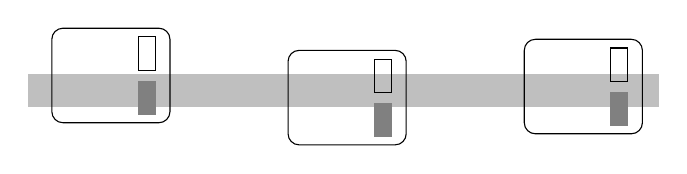
\begin{tikzpicture}
	\draw[fill,lightgray] (0,0) rectangle +(8,4mm);
	\foreach \x/\y in {6.5cm/1pt, .5cm/5pt, 3.5cm/-3pt} {
		\draw[rounded corners] (\x-2mm,\y-11pt) rectangle +(15mm,12mm);
		\draw[fill,gray] (\x+.9cm,\y-8pt) rectangle +(6pt,12pt);
		\draw (\x+.9cm,\y+8pt) rectangle +(6pt,12pt);
	}
	\end{tikzpicture}
\end{center}

\bigskip

{\raggedleft \hfill Beispielprogramm \bu{line-one.aesl}}
\chap{Multiple Thymios}\label{ch.two}

You can run two or more Thymio robots at the same time.

\textbf{Specification}

Place two robots T1 and T2 facing each other. T1 chases T2; when
T1 detects that it is close to T2 it will stop. If T2 detects that T1 is
close to it, T2 retreats until it no longer detects T1. 

\textbf{Guidance}

\begin{itemize}

\item The programs for T1 and T2 have two event-action pairs: one whose
event is the detection of an object by the center horizontal sensor, and
another whose event is the non-detection of an object. However, the
actions for T1 and T2 are different.

\item Connect two Thymios T1 and T2 to the computer and turn them on.
Run two copies of VPL. In the target-selection window
(Figure~\ref{fig.connect}), both T1 and T2 should appear; select T1 in
one copy of VPL and T2 in the other. Open and run program \p{chase} in
T1 and program \p{retreat} in T2.
 
\end{itemize}

\textbf{Experiments}

\begin{itemize}

\item What happens if you exchange the programs: T1 runs
\p{retreat} and T2 runs \p{chase}? Explain.

\item In advanced mode, experiment with different settings of the sensor
thresholds.

\end{itemize}

%\bigskip

{\raggedleft \hfill Program file \bu{chase.aesl}, \bu{retreat.aesl}}

\bigskip

\informationbox{Communications between robots}{Multiple Thymio robots
can send messages to each other. This capability is supported in the
AESL language and Studio environment.}

\part{From visual to textual programming}

\chap{Learning AESL from VPL programs}\label{ch.next}


Congratulations! You are an expert in programming the Thymio robot using
the \textit{Visual Programming Environment (VPL)}. Now you want to move
on and use the professional \textit{Studio Programming Environment}
(\cref{fig.studio}) and its textual programming language, the
\textit{Aseba Event Scripting Language (AESL)}.

\begin{figure}[hbt]
\begin{center}
\gr{studio}{.9}
\caption{Aseba Studio environment}\label{fig.studio}
\end{center}
\end{figure}

VPL translates graphical programs (event-actions pairs) into a textual
AESL program, which is displayed in the right-hand panel of the VPL
window (panel~6 in \cref{fig.vplgui} on page~\pageref{fig.vplgui}). This tutorial uses VPL programs
from the previous chapters of this tutorial and explains the
corresponding AESL program. You will be able to use your understanding
of the VPL program to learn the fundamental concepts of AESL
programming.

Programming in Aseba Studio is also based upon the concepts of events
and actions. Since VPL programs are translated into AESL programs,
everything you learned in this tutorial is supported in Studio, but now
you have the flexibility of a full programming language with variables,
expressions, and control statements.

When you are working with Aseba Studio, you can open VPL by clicking on
the button \bu{Launch VPL} in the \emph{Tools} tab at the bottom left of
the window. You can import VPL programs into Aseba Studio simply by
opening its file.

Sections marked $^*$ present AESL programming concepts that
go beyond what is found in the VPL projects. They can be skipped when
you first read this tutorial.

\newpage

\textbf{\large Documentation}

To learn about Aseba Studio and AESL, go to the \emph{Programming
Thymio} page at\\
\href{https://www.thymio.org/en:asebausermanual}{https://www.thymio.org/en:asebausermanual}.
You can find documentation of:

\begin{itemize}
\item The Studio programming environment.
\item The AESL programming language.
\item The interface to the Thymio robot.
(There is a reference card for the interface).
\item The native functions library supported in AESL.
\end{itemize}

There is also an archive describing interesting projects in AESL,
together with the source of proposed solutions.

\sect{The Thymio Interface}

Here is the program \p{whistles.aesl} from \cref{ch.bells} together with
part of the corresponding AESL program:
 
\begin{center}
\begin{tabular}{ll}
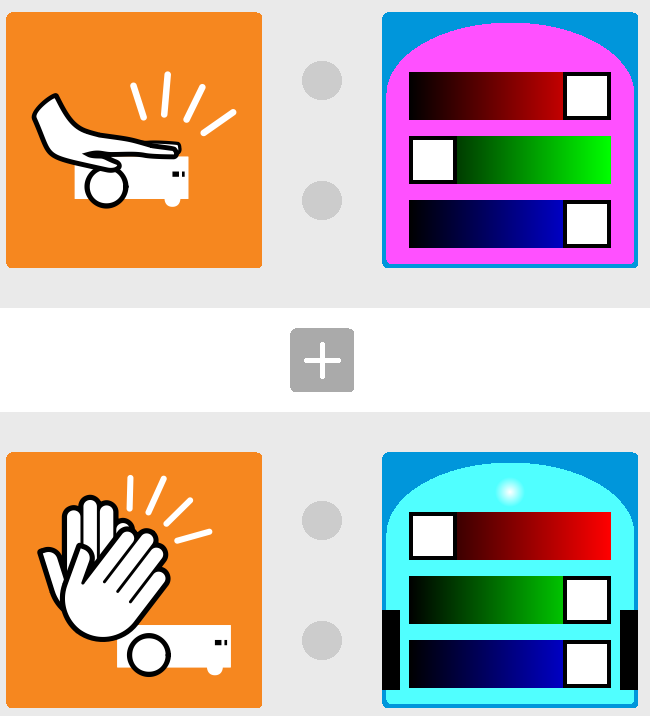
\includegraphics[width=.4\textwidth]{whistles} &
\begin{minipage}[b]{.5\textwidth}
\begin{footnotesize}
\begin{verbatim}
  onevent tap
    call leds.top(32,0,32)
  
  onevent mic
    call leds.bottom.left(0,32,32)
    call leds.bottom.right(0,32,32)
\end{verbatim}
\end{footnotesize}
\vspace*{8ex}
\end{minipage}
\end{tabular}
\end{center}

\textbf{\large Event handlers}

When a tap event occurs, the top light is turned on with the color
called \emph{magenta}, and when the clap event occurs, the bottom light
is turned on with the color called \emph{cyan}. Corresponding to the
event-actions pairs in VPL are \emph{event handlers}, which are
introduced by the keyword \p{onevent} (read this as two words: ``on
event''). You can find a list of events in the table at the bottom of
the documentation for the Thymio programming interface.

The lines following \p{onevent} form the body of the event handler
and correspond to the action blocks to the right of an event block in VPL.

When a tap event occurs, the \emph{interface function} \p{leds.top} is
\emph{called}. The function takes three \emph{parameters}, which specify
the intensities of the red, green and blue components of the LED.
Their values can range from 0 (off) to 32 (full). The combination of red
and blue gives magenta.

The VPL clap event corresponds to the \p{mic} event (short for
microphone). When the event occurs, the bottom LEDs are turned on. In
VPL, one action block turns on both LEDs to the same color, whereas in
AESL, the left and right LEDs can be set separately. Here, we set both
of them to full intensity of green and blue, giving cyan.

\textbf{\large Assigning a value to a variable}

Look again at the AESL program in the VPL window. The first two lines are:
\begin{footnotesize}
\begin{verbatim}
  # setup threshold for detecting claps
  mic.threshold = 250
\end{verbatim}
\end{footnotesize}

A line beginning with \verb+#+ is called a \emph{comment}. Comments do
not affect the running of a program; they are used to give information
to the reader of the program. Here, the comment notes that the clap
event occurs when the intensity of the sound is greater than a
\emph{threshold}. The second line of the program specifies that the
event occurs when then intensity of the sound (which can be in the range
$0$--$255$) is greater than $250$.

In VPL, the threshold is built-in and cannot be changed, but in a
textual program you can change it using an \emph{assignment statement}:
\begin{footnotesize}
\begin{verbatim}
  mic.threshold = 180
\end{verbatim}
\end{footnotesize}
Its meaning is that the \emph{value} on the right-hand side of the
\verb+=+ symbol is copied to the \emph{variable} on the left-hand side.
The variable \p{mic.threshold} is predefined for the Thymio robot.

\textbf{\large Initialization of the Thymio}

At the beginning of each program, VPL automatically inserts a sequence
of statements that turns off all the LEDs and the sound:

\begin{footnotesize}
\begin{verbatim}
  # reset outputs
  call sound.system(-1)
  call leds.top(0,0,0)
  call leds.bottom.left(0,0,0)
  call leds.bottom.right(0,0,0)
  call leds.circle(0,0,0,0,0,0,0,0)
\end{verbatim}
\end{footnotesize}

This \emph{initialization} is not visible in the VPL program. In a
textual program, it is recommended that you include these statements,
but it is not required.

\newpage

\sect{Alternatives}

The program \p{colors-multiple.aesl} from \cref{ch.colors} changes the
colors of the top and bottom LEDs when the buttons are touched:

\begin{center}
\begin{tabular}{ll}
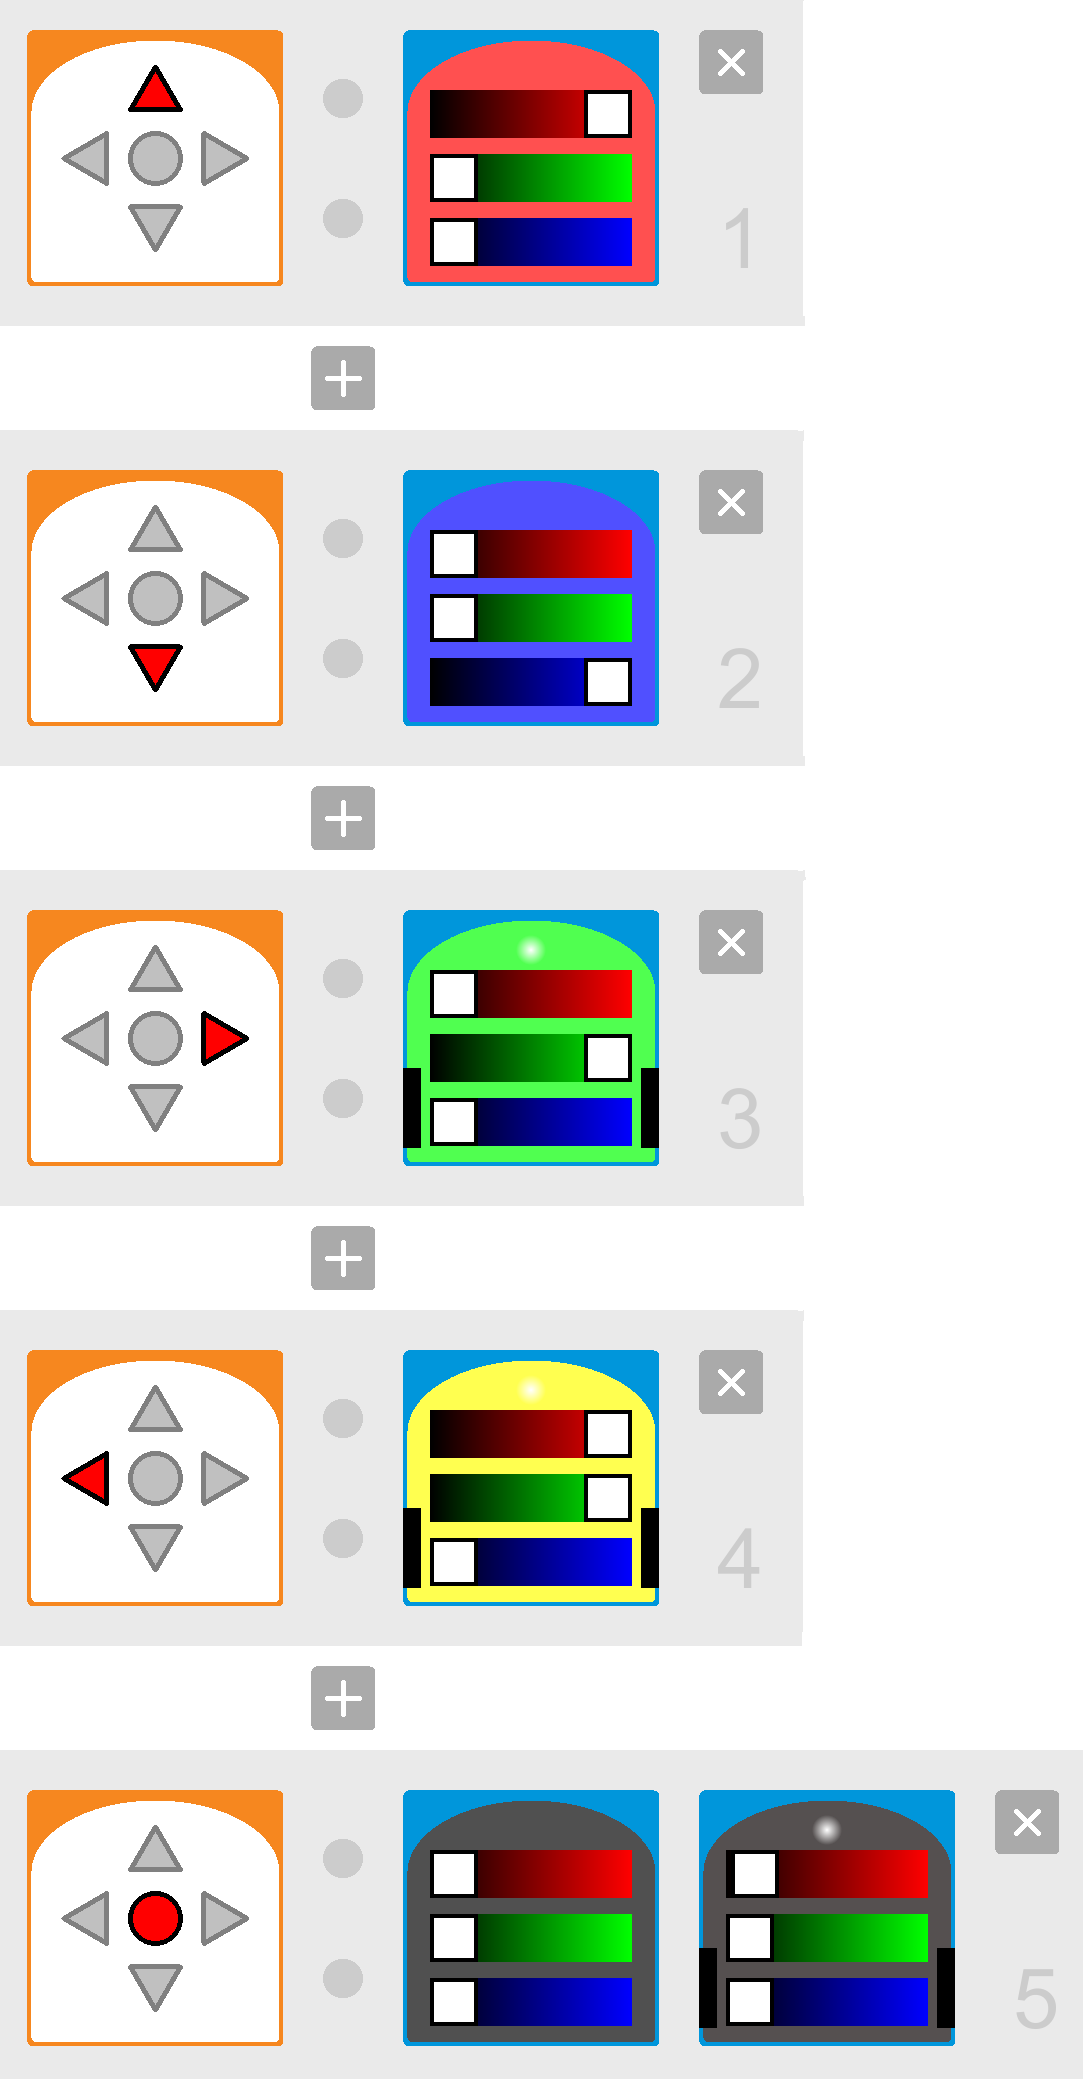
\includegraphics[width=.4\textwidth]{colors-multiple-full} &
\begin{minipage}[b]{.5\textwidth}
\begin{footnotesize}
\begin{verbatim}
  onevent buttons
    when button.forward == 1 do
      call leds.top(32,0,0)
    end
    when button.backward == 1 do
      call leds.top(0,0,32)
    end
    when button.right == 1 do
      call leds.bottom.left(0,32,0)
      call leds.bottom.right(0,32,0)
    end
    when button.left == 1 do
      call leds.bottom.left(32,32,0)
      call leds.bottom.right(32,32,0)
    end
    when button.center == 1 do
      call leds.top(0,0,0)
      call leds.bottom.left(7,0,0)
      call leds.bottom.right(7,0,0)
    end
\end{verbatim}
\end{footnotesize}
\vspace*{5ex}
\end{minipage}
\end{tabular}
\end{center}

In the AESL program, a \emph{single} event occurs when any of the five
buttons is touched. The action of the event handler \p{onevent buttons}
depends on which button is touched, so we check the value of the
\emph{button variables} in order to select an action. The statements:

\begin{footnotesize}
\begin{verbatim}
  when button.forward == 1 do
    call leds.top(32,0,0)
  end
\end{verbatim}
\end{footnotesize}

mean: \emph{when} the value of the variable \p{button.forward} changes
from some other value (here, 0) to 1, \emph{then} perform the actions
written on the lines between the keyword \p{do} and the keyword \p{end}.
There are five \p{button} variables, one for each button. The value of a
button variable is 1 if the button is touched and 0 if the button is
released. In the program, there are five \p{when}-statements, one for
each button. One or two actions are run if the expression in a
\p{when}-statement \emph{becomes} true.

\textbf{\large One event or multiple events$^*$}

The Thymio interface includes separate events for each button, in
addition to the \p{buttons} event that occurs if any button is touched
or released. We could implement the program as follows, using multiple
events without \p{when}-statements and button variables:

\begin{footnotesize}
\begin{verbatim}
  onevent button.forward
    call leds.top(32,0,0)
  
  onevent button.backward
    call leds.top(0,0,32)
  
  onevent button.right
    call leds.bottom.left(0,32,0)
    call leds.bottom.right(0,32,0)
  
  onevent button.left
    call leds.bottom.left(32,32,0)
    call leds.bottom.right(32,32,0)
  
  onevent button.center
    call leds.top(0,0,0)
    call leds.bottom.left(1,0,0)
    call leds.bottom.right(1,0,0)
\end{verbatim}
\end{footnotesize}

The advantage of using separate events is that the program is easier to
read and understand, but there are cases where you need to use the event
\p{buttons}: (a) to distinguish between touching and releasing a button,
and (b) to identify touching two buttons at once:

\begin{footnotesize}
\begin{verbatim}
  onevent buttons
    # Turn the top LEDs on when the forward button is released
    when button.forward == 0 do
      call leds.top(32,0,0)
    end

    # Turn the bottom LEDs on when
    #   both the left and the right buttons are  touched
    when button.left == 1 and button.right == 1 do
      call leds.bottom.left(0,32,0)
      call leds.bottom.right(0,32,0)
    end
\end{verbatim}
\end{footnotesize}


Another difference is that the individual events occur when a button is
touched or released, whereas the common event \p{buttons} occurs with a
frequency of 20 Hz after updating the array of button variables (see
page~\pageref{pg.hz} for an explanation of these concepts).


\textbf{\large \p{if}-statements}\label{p.if-when}

AESL supports two alternative statements:
\begin{footnotesize}
\begin{verbatim}
  when v == 1 do ... statements ... end

  if v == 1 then ... statements ... end
\end{verbatim}
\end{footnotesize}
that have different meanings:
\begin{quote}
\emph{when} the value of \p{v} \emph{becomes} 1, run the statements

\emph{if} the value of \p{v} \emph{is} 1, run the statements
\end{quote}

\p{when}-statements are commonly used with variables representing
events, because we usually want to run an event handler when something
changes, not just because the value of a variable has a certain value.
We could write a \p{buttons} event handler using an \p{if}-statement:

\begin{footnotesize}
\begin{verbatim}
  onevent buttons
    if button.forward == 1 then
      ... statements ...
    end
\end{verbatim}
\end{footnotesize}
However, if we touch the forward button for a long period of time,
the statements would be run several times. If the statements change the
color of the LEDs, it wouldn't make a difference, but there are cases
where it does matter and a \p{when}-statement is needed.

An \p{if}-statement is appropriate when we are interested the values of
variables and not in their changes. The following statements set the
value of the variable \p{max} to the maximum value returned by the two
rear sensors:

\begin{footnotesize}
\begin{verbatim}
  if prox.horizontal[5] > prox.horizontal[6] then
    max = prox.horizontal[5]
  else
    max = prox.horizontal[6]
  end
\end{verbatim}
\end{footnotesize}

Additional examples of \p{if}-statements appear in the next section and
in Figure~\ref{fig.respond}.


\newpage

\sect{Arrays}

The program \p{likes.aesl} in \cref{ch.pet} of the VPL tutorial causes the
robot to follow your hand as you move it from side to side near the
forward horizontal proximity sensors.
When an object is not detected, the robot stops; when an object is
detected in front of the center sensor, the robot moves forward; when an
object is detected in front of the leftmost or rightmost sensor, the
robot turns in that direction.

\begin{figure}[hbt]
\begin{center}
\begin{tabular}{lr}
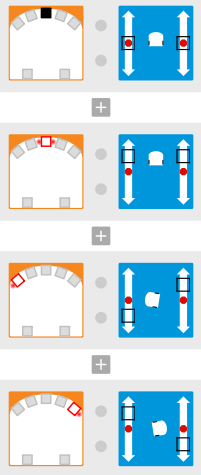
\includegraphics[width=.35\textwidth]{likes} &
\begin{minipage}[b]{.4\textwidth}
\begin{footnotesize}
\begin{verbatim}
  onevent prox
    when prox.horizontal[2] < 1000 do
      motor.left.target = 0
      motor.right.target = 0
    end
    when prox.horizontal[2] > 2000 do
      motor.left.target = 300
      motor.right.target = 300
    end
    when prox.horizontal[0] > 2000 do
      motor.left.target = -300
      motor.right.target = 300
    end
    when prox.horizontal[4] > 2000 do
      motor.left.target = 300
      motor.right.target = -300
    end
\end{verbatim}
\end{footnotesize}
\end{minipage}
\end{tabular}
\caption{The \p{likes} program in VPL and AESL}\label{fig.arrays}
\end{center}
\end{figure}

The AESL program (\cref{fig.arrays}) is structured as an event handler
with several \p{when}-statements. The values of the motor variables
\p{motor.left.target} and \p{motor.right.target} are set to values
corresponding to the positions of the sliders in the motor blocks. In
VPL, the sliders change the values of the motor variables in increments
of $50$, but in AESL you can set them to any values in the range $-500$
to $500$.

The event is called \p{prox}. Unlike the button events, which
occur when something ``happens,'' this event occurs \emph{10 times
every second}. Before the event occurs, the values of the
\p{prox.horizontal} variables are set to values that depend on what the
sensors are detecting. See the\label{pg.hz} documentation of the
Thymio programming interface for details.\footnote{The unit
for \emph{frequency}, the number of times something happens per second, is called
the \emph{hertz}, abbreviated \emph{Hz}. The interface document specifies
that the {\footnotesize\p{prox}} event occurs with frequency \emph{10 Hz}.}

\textbf{\large Arrays as multiple variables}

The Thymio robot has 7 horizontal proximity sensors, 5 in front and 2 in
the back. To read the values detected by the sensors, it would be
possible to define 7 different variables:

\begin{footnotesize}
\begin{verbatim}
  prox.horizontal.front.0
  prox.horizontal.front.1
  prox.horizontal.front.2
  prox.horizontal.front.3
  prox.horizontal.front.4
  prox.horizontal.back.0
  prox.horizontal.back.1
\end{verbatim}
\end{footnotesize}

Instead, AESL enables you to define an \emph{array}, which is a sequence
of variables all with the same name. The different variables in the
sequence are identified with a number. The array for the horizontal
proximity sensors is predefined and is called \p{prox.horizontal}:

\begin{center}
\begin{picture}(240,40)
\put(0,0){\makebox(100,20)[l]{\p{prox.horizontal}}}
\put(100,0){\framebox(140,20){}}
\multiput(120,0)(20,0){6}{\line(0,1){20}}
\put(100,20){\makebox(20,20){\p{0}}}
\put(120,20){\makebox(20,20){\p{1}}}
\put(140,20){\makebox(20,20){\p{2}}}
\put(160,20){\makebox(20,20){\p{3}}}
\put(180,20){\makebox(20,20){\p{4}}}
\put(200,20){\makebox(20,20){\p{5}}}
\put(220,20){\makebox(20,20){\p{6}}}
\end{picture}
\end{center}

The first 5 components are for the front sensors from left to right,
while the last two components are for the back sensors from left to
right. If you don't remember the assignment of numbers to sensors, you
can always look it up in the the documentation for the Thymio
programming interface, even better, on the diagram in the reference
card.

To access a specific component in an array, write its sequence number in
square brackets after the name of the array variable. This number is
called an \emph{index} into the array. The following statement specifies
that the motor variables will be set to 300 when the value of the
\emph{front center sensor} (index 2) becomes greater than 2000:

\begin{footnotesize}
\begin{verbatim}
  when prox.horizontal[2] > 2000 do
    motor.left.target = 300
    motor.right.target = 300
  end
\end{verbatim}
\end{footnotesize}

Later, we will see that array variables can have their
values set in an assignment statement:
\begin{footnotesize}
\begin{verbatim}
  timer.period[0] = 1979
\end{verbatim}
\end{footnotesize}

\textbf{\large \p{for}-loops and index variables$^*$}

A natural generalization of arrays is to use a variable instead of a
constant for the index.\footnote{This is not used in translations of VPL
programs into AESL, except in an advanced construct for constructing
sounds; therefore, the simple example here is taken from the AESL
projects.} The program \p{cats.aesl} contains the following statements:

\begin{footnotesize}
\begin{verbatim}
  var i

  for i in 0:4 do
    if prox.horizontal[i] > DETECTION then
      state = 2
    end
  end
\end{verbatim}
\end{footnotesize}

Previously, we only used variables that are built into the Thymio
interface; here, the first line \emph{declares} a new variable called
\p{i}. The next statement is a \p{for}-statement whose meaning is:

\begin{itemize}
\item Assign the values 0, 1, 2, 3, 4 in turn to the variable \p{i};
\item For each assignment, run the statements between \p{do} and \p{end}.
\end{itemize}

Here, there is a single \p{if}-statement between \p{do} and \p{end}. It
checks the value of the horizontal proximity sensors and sets the value
2 in the variable \p{state} if the value read from a sensor is greater
than the constant \p{DETECTION}.\footnote{See the documentation of the 
Aseba Studio environment for instructions on how to define constants.}

The variable \p{i} receives the values 0, 1, 2, 3, 4 in turn, so each
time the \p{if}-statement is run, \p{prox.horizontal[i]} reads the value
of each front sensor from left to right. The result of the
\p{for}-statement is thus to set the value of the variable \p{state} to
2 \emph{if} \emph{any} of the front sensors detects an object.

\textbf{\large Declaring an array}

An array variable is declared by giving its size in brackets following
the array name. The size can also be specified by providing an initial
value:\footnote{A comment need not start at the beginning of a line.
Every character from the symbol \# to the end of the line is considered
to be a comment and is ignored by the computer.} 

\begin{footnotesize}
\begin{verbatim}
var state[4]             # An array with four components
var state[] = [0,0,0,0]  # An array with four components
\end{verbatim}
\end{footnotesize}

In the translation of the VPL program, both the size and the initial
value are given. This is correct as long as the number of values is the
same as the size:

\begin{footnotesize}
\begin{verbatim}
var state[4] = [0,0,0,0]  # OK, but redundant
\end{verbatim}
\end{footnotesize}

\newpage

\sect{Timers}

\cref{ch.time} introduced \emph{timers}. The program
\p{shy.aesl} causes the robot to turn left when the front center sensor
detects your hand; two seconds later, it turns right:

\begin{center}
\begin{tabular}{ll}
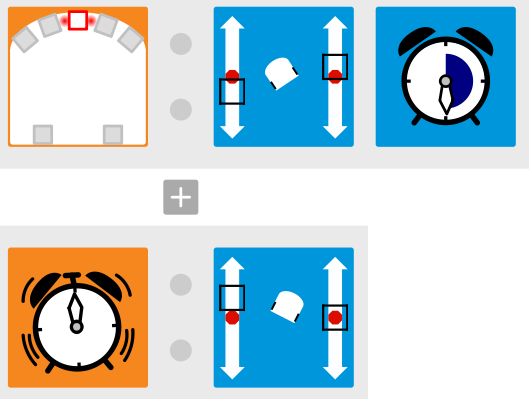
\includegraphics[width=.4\textwidth]{shy} &
\begin{minipage}[b]{.5\textwidth}
\begin{footnotesize}
\begin{verbatim}
  onevent prox
    when prox.horizontal[2] > 2000 do
      motor.left.target = -150
      motor.right.target = 100
      timer.period[0] = 2000
    end
  
  onevent timer0
    timer.period[0] = 0
    motor.left.target = 200
    motor.right.target = 0
\end{verbatim}
\end{footnotesize}
%\vspace*{1ex}
\end{minipage}
\end{tabular}
\end{center}

There are two timers in the Thymio robot. You set the duration of a
timer by assigning a value to components 0 or 1 of the array
\p{timer.period}. The value is in \emph{milliseconds}, thousandths of a
second. To set a duration of 2 seconds in timer 0, the value 2000
(milliseconds) should be assigned to \p{timer.period[0]}.

There are two events, \p{timer0} and \p{timer1}, one for each timer.
When the duration has passed (we say that the timer has \emph{expired}),
the timer event occurs. In the handler for the event \p{timer0}, we set
the timer duration to 0 so it won't occur again and change the motor
settings.

As part of its initialization, the program sets the timer to 0 so that
the event won't accidently occur at the beginning of the program:

\begin{footnotesize}
\begin{verbatim}
  # stop timer 0
  timer.period[0] = 0
\end{verbatim}
\end{footnotesize}

\newpage

\sect{States}

\cref{ch.states,ch.counting} showed how to use \emph{states}. The
Thymio robot can be in one of 16 states and you can specify that an
event causes an action only if the robot is in certain states. In the
program \p{count-to-two.aesl} from \cref{ch.counting}, the state is set to 0 when
the center button is touched and then it counts whether the number of
claps is even or odd by alternating between state 0 and state 1. The VPL
program and the AESL event handler for touching the center button
are:\footnote{The AESL program shown here is different from the one
generated by VPL as explained later in this chapter.}

\begin{center}
\begin{tabular}{ll}
\raisebox{8ex}{
\includegraphics[width=.4\textwidth]{two-button}} &
\begin{minipage}[b]{.5\textwidth}
\begin{footnotesize}
\begin{verbatim}
  var state[] = [0,0,0,0]
  
  onevent buttons
    when button.center == 1 do
      state[0] = 0
      state[1] = 0
      state[2] = 0
      state[3] = 0
    end
\end{verbatim}
\end{footnotesize}
\end{minipage}
\end{tabular}
\end{center}

The state is stored in an array \p{state[]} which has 4 components. Each
component can be 0 or 1, so there are $2\times 2\times 2\times 2=16$
possible values in the array. The components of the array are given
initial values of 0 by assigning the four values
{\footnotesize\verb+[0,0,0,0]+}. The initial value of the array is also
used to specify the number of components in an array; since there are 4
values in {\footnotesize\verb+[0,0,0,0]+}, there are 4 components in the
array.

The state event block (green, next to the button event block) has all of
its quarters set to gray; this means that the event can occur regardless
of the current value of the state. Therefore, whenever the center button
is touched, the state action block (blue) causes all the components of
the array \p{state} to be set to 0, as indicated by the white quarters.
In the corresponding AESL program, the \p{when}-statement checks if the
button was touched, but does not check the value of the array \p{state}.
If the button was touched, each component of the array is set to 0.

There are two clap event blocks, each one associated with a different
state block. In the textual program a single \p{mic} event handler will
be used. The statements to be run will depend on \p{if}-statements
(\cref{fig.respond}).

\begin{figure}[hbt]
\begin{center}
\begin{tabular}{ll}
\raisebox{10ex}{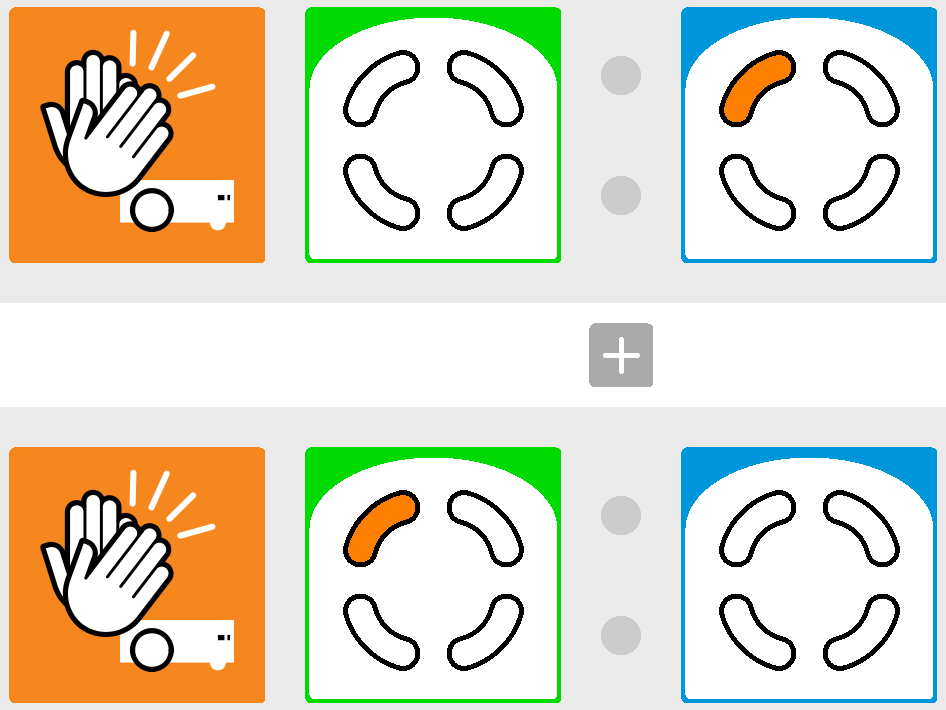
\includegraphics[width=.4\textwidth]{two-clap}} &
\begin{minipage}[b]{.5\textwidth}
\begin{footnotesize}
\begin{verbatim}
  onevent mic
    if state[0] == 0 and
       state[1] == 0 and
       state[2] == 0 and
       state[3] == 0 then
      state[0] = 1
      state[1] = 0
      state[2] = 0
      state[3] = 0
    end
    if state[0] == 1 and
       state[1] == 0 and
       state[2] == 0 and
       state[3] == 0 then
      state[0] = 0
      state[1] = 0
      state[2] = 0
      state[3] = 0
    end
\end{verbatim}
\end{footnotesize}
\end{minipage}
\end{tabular}
\caption{Responding to claps according to the state}\label{fig.respond}
\end{center}
\end{figure}

The meaning of the keyword \p{and} is that \emph{all} the conditions in
the \p{if}-statement must hold in order to run the statements between
\p{then} and \p{end}. If all components of \p{state} are 0, the value of
\p{state[0]} is set to 1, while the others are set to 0. This
corresponds to the state event block having all quarters white and the
state action block having the upper left quarter orange and the others
white. Similarly, if value of \p{state[0]} is 1 and the values of the
other components are 0, the values of all the components of \p{state}
are set to 0.\footnote{In the state action block, it would be sufficient just to change the upper left quadrant and gray the other quadrants since their values don't change. However, errors are less likely if we explicitly give values (orange or white) to each of the quadrants.}

\newpage

\sect{Subroutines}

Quite often we need to run the same sequence of statements from many
places within a program. We could write the statements once and copy
them each time they are needed. A simpler solution is to use a
\emph{subroutine}, which assigns a name to a sequence of statements. In
this program, the declaration {\footnotesize\verb+sub display_state+}
declares a subroutine that assigns the name
{\footnotesize\verb+display_state+} to a sequence of statements, here,
the single statement \p{call leds.circle}:

\begin{footnotesize}
\begin{verbatim}
  # subroutine to display the current state
  sub display_state
    call leds.circle(
      0, state[1]*32, 0, state[3]*32, 0, state[2]*32, 0, state[0]*32)
\end{verbatim}
\end{footnotesize}

When the subroutine is \emph{called}, it runs the statements assigned to
the name of the subroutine:
\vspace{-1ex}
\begin{footnotesize}
\begin{verbatim}
  callsub display_state
\end{verbatim}
\end{footnotesize}
\vspace{-1ex}
The interface function \p{leds.circle} sets the eight curved LEDs
surrounding the buttons. You really do need to refer to the cheat sheet
to learn which parameter sets which LED!

The intensity of each LED is set by giving the corresponding parameter a
value between 0 (off) and 32 (full intensity). The front, back,
left and right LEDs are set to 0 (off), whereas the diagonal LEDs are
set to on if the corresponding state component is 1 and off if the state
component is 0. This is achieved by the \emph{arithmetic expressions}
\p{state[...]*32} which multiply the value of the components of the array
by 32. If one of the values is 0, the result is 0, while if it is 1, the
result is 32.

\newpage

\sect{Native functions}

The program above has a problem. Since the components of the array
\p{state} are set one-by-one, it is possible that an different event
will occur when some, but not all, of the components have been set. To
set all the components at once, the new values of the state are first
set in a second array \p{new\_state} and then they are copied to the
first array \p{state}:

\begin{footnotesize}
\begin{verbatim}
# variables for state
var state[4] = [0,0,0,0]
var new_state[4] = [0,0,0,0]

onevent buttons
  when button.center == 1 do
    new_state[0] = 0
    new_state[1] = 0
    new_state[2] = 0
    new_state[3] = 0
  end

  call math.copy(state, new_state)
  callsub display_state
\end{verbatim}
\end{footnotesize}

The \emph{native function} \p{math.copy} is used to copy the arrays.
Native functions are built into the Thymio robot and are more efficient
than sequences of statements in AESL. The native functions are described
in the Aseba documentation.

The current version of AESL allows assignment of entire arrays, so that
it would have been possible to use the assignment
statement:\footnote{The array assignment translates into a sequence of
individual assignment statements, one for each component, so nothing is
actually gained by using an array assignment statement.}

\begin{footnotesize}
\begin{verbatim}
  state = new_state
\end{verbatim}
\end{footnotesize}

\appendix
\part{Anhänge}

\chap{Die VPL Benutzer-Schnittstelle}\label{a.toolbar}

Zuoberst im VPL-Fenster hat es eine Werkzeugleiste (Toolbar):

\begin{center}
\gr{toolbar}{1}
\end{center}

\bigskip

\textbf{Neu} \blksm{new}: Löscht den bisher programmierten Code und stellt eine leere Programmierumgebung dar.

\bigskip

\textbf{Öffnen} \blksm{open}: Klicken Sie, um ein bestehendes VPL-Programm zu öffnen. Ein Fenster wird erscheinen und Sie können durch die Ordner navigieren zum Verzeichnis, wo Sie Ihre Programmdateien gespeichert haben (Datei-Erweiterung \p{aesl}).

\bigskip

\textbf{Speichern} \blksm{save}: Speichert das aktuelle Programm. Es ist eine gute Idee, diesen Knopf regelmässig zu betätigen, damit Sie Ihre Arbeit nicht verlieren, wenn ein Fehler auftritt. 

\bigskip

\textbf{Speichern als} \blksm{saveas}: Speicher das aktuelle Programm unter einem \emph{anderen Namen}. Benutzen Sie ''Speichern als'' wenn Sie in einem Programm etwas ausprobieren wollen und das bisherige Programm nicht verlieren wollen. 

\bigskip

\textbf{Zurücksetzen} \blksm{undo} (undo): Mit ''Zurücksetzen'' oder auch ''rückgängig machen'' werden getätigte Eingaben rückgängig gemacht (wie z.B. das Löschen eines Ereignis-Aktions-Paares)\label{p.undo}

\bigskip

\textbf{Vorwärts machen} \blksm{redo} (redo): Mit ''Vorwärts machen'' oder ''Wiederholen'' wird eine Eingabe, die mit ''Zurücksetzen'' rückgängig gemacht wurde, erneut ausgeführt. 

\bigskip

\textbf{Laden und ausführen} \blksm{run} (run): Kompiliert das Programm, lädt es auf den Roboter und führt es aus. Die Übertragung geschieht nur, das Programm korrekt kompiliert werden konnte. Wenn Sie das Programm geändert haben, blinkt der Knopf grün um Sie daran zu erinnern, dass Sie das geänderte Programm erneut kompilieren und übertragen müssen. 

\bigskip

\textbf{Halten} \blksm{stop}(stopp): Stoppt das laufende Programm und lässt den Roboter anhalten. Verwenden Sie diesem Knopf um den Roboter anzuhalten, wenn es kein Ereignis-Aktions-Paar gibt, das den Roboter anhalten lässt. 

\bigskip

\textbf{Fortgeschrittener Modus} \blksm{advanced}: Der fortgeschrittene Modus aktiviert zusätzliche Elemente und Optionen wie Zustände, Timer, Beschleunigungssensoren und Sensor-Grenzwerte. Der Knopf ändert die Farbe in orange.

\textbf{Standard-Modus}: Der selbe Knopf \blksm{basic} wird betätigt, um wieder zurück in den Standard-Modus zu wechseln (die Farbe wechselt wieder zurück in blau). 

\textbf{Hilfe} \blksm{info1}: Stellt in einem Internet-Browser-Fenster die VPL-Dokumentation unter folgendem Link dar: \href{https://www.thymio.org/en:thymiovpl}{https://www.thymio.org/en:thymiovpl}. Eine Internetverbindung ist nötig!

\bigskip

\textbf{Bildschirmfoto} \blksm{export}: \label{p.export} Exportiert ein Bild vom aktuellen VPL-Programm. Sie können dieses Bild dann in ein beliebiges Dokument integrieren. Verschiedene Grafikformate stehen zur Verfügung; \textsc{svg} ergibt die höchste Qualität, aber \textsc{png} ist wohl am weitesten verbreitet.

%\section*{Feedback}

%(To be written)

%\label{p.feedback}

\chap{Summary of VPL Blocks}\label{a.blocks}

\sect{Event blocks}

\blksm{event-buttons} \textbf{Buttons}. Click on one or more of the images
of the buttons; they will turn red. An event will occur if the red
buttons are touched.

\bigskip\bigskip


\blksm{event-prox} \textbf{Horizontal sensors} (five at the front of the
Thymio and two at the back). Click on one or more of the small squares
and they will change color. Initially, all squares are gray, meaning
that the reading of each sensor is ignored.

If the square is white with a red border \blksm{center-prox}, an event
occurs if a lot of light is reflected.

If the square is black \blksm{center-no-prox}, an event occurs if little
light is reflected.

\bigskip

\trickbox{Ordinary objects need to be very close to the Thymio before they are
detected by the horizontal sensors. You can greatly increase
the range by attaching \emph{reflector tape}, such as used on bicycles,
to the objects.\footnote{My thanks to Francesco Mondada for showing this
to me!}\\
Compare the following image with \cref{fig.cat-mouse}:
\begin{center}
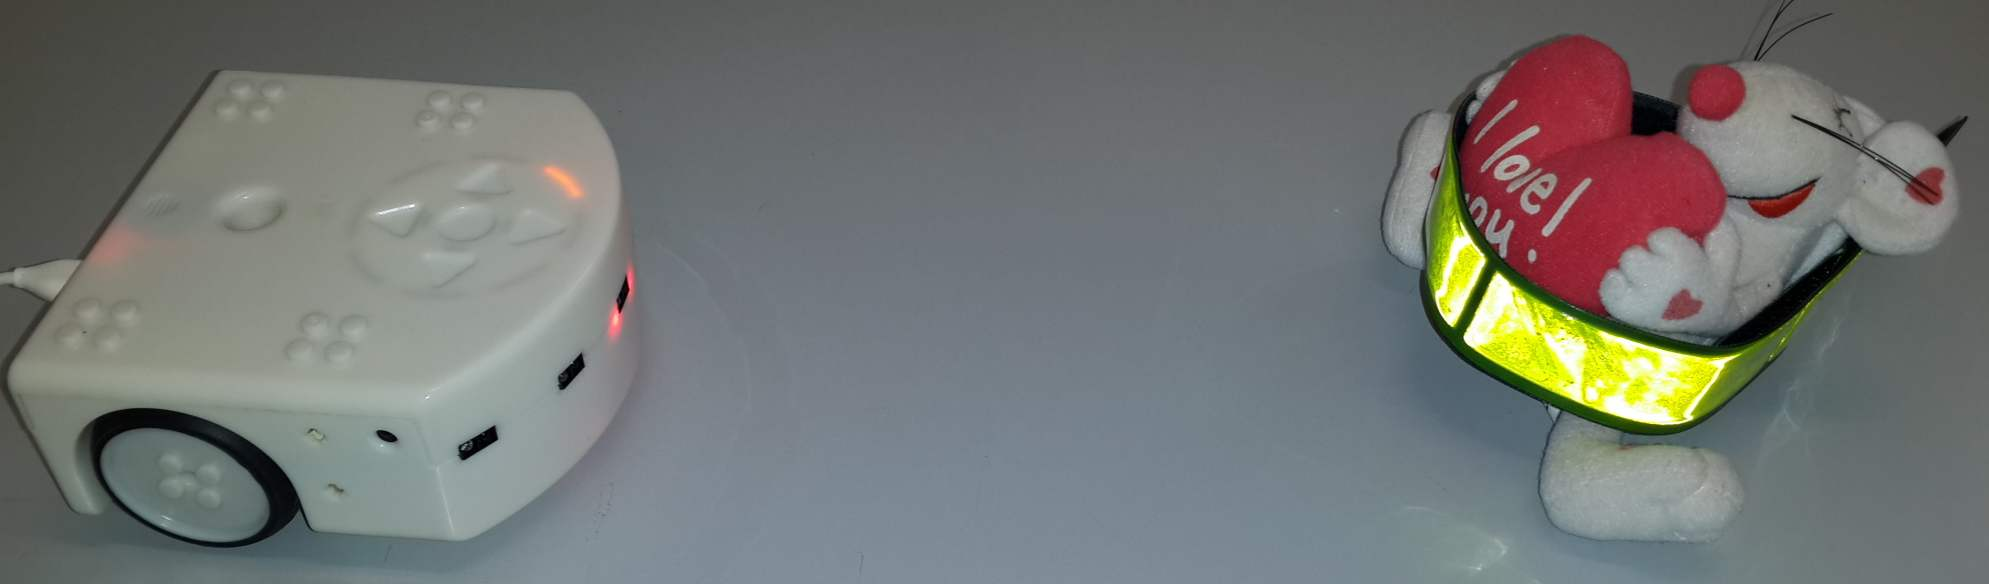
\includegraphics[width=0.8\textwidth]{reflect}
\end{center}
}

\bigskip

\blksm{event-prox-ground} \textbf{Ground sensors} (two on the bottom of the
Thymio). Use like the block for the horizontal sensors.

\bigskip\bigskip

\blksm{event-prox-advanced}, \blksm{event-prox-ground-advanced}
\textbf{Sensors, advanced mode}. Use like the previous blocks. The top
slider sets the threshold above which an object is detected and the
bottom slider sets the threshold below which the absence of an object is
detected.

\bigskip\bigskip

There is an additional mode (the square is dark gray \blksm{slow-mid})
in which an event occurs if the value is between to upper and lower
threshold.

\bigskip\bigskip\bigskip

\blksm{event-tap} \textbf{Tap}. An event occurs when the Thymio is
tapped.

\bigskip\bigskip\bigskip

\blksm{event-tap-advanced} \textbf{Tap, advanced mode}. Use like the
previous block. Click on the small center or right circle to change to
an accelerometer event.

\bigskip\bigskip

\blksm{event-roll}, \blksm{event-pitch} \textbf{Accelerometer,
advanced mode}. Drag the white angle segment on the half-circle left or right.
An event will occur if the left / right or forwards / backwards angle
(respectively) of the Thymio is within the segment.

\bigskip\bigskip\bigskip\bigskip

\blksm{event-timer} \textbf{Timer, advanced mode}. An event occurs when
a timer has counted down to zero. The timer must have been set by a
previous timer \emph{action}.

\bigskip\bigskip\bigskip

\blksm{event-state} \textbf{State event, advanced mode}. The event
occurs only if the components of the current state match the
corresponding orange and white quarters of this block. The components
corresponding to the gray quarters need not match.

\bigskip

\sect{Action blocks}

\blksm{action-motors} \textbf{Motors}. Move the left and right sliders
up to increase the forwards rotation of the left and right motors,
respectively, and move the sliders down to increase the backwards
rotation.

\bigskip\bigskip

\blksm{action-colors-up} \textbf{Top lights}. Move the three sliders to
the right to increase the red, green and blue components of the top
light, respectively.

\bigskip\bigskip

\blksm{action-colors-down} \textbf{Bottom lights}. Turns the bottom
lights on. Use like the previous block.

\bigskip\bigskip

\blksm{action-music} \textbf{Music}. The six small circles are notes. A
black circle is a short note, a white circle is a long note and a blank
is a rest. Click on a circle to change the length. The five horizontal
bars, represent tones. Click on the bar to move a circle to that bar.

\bigskip\bigskip

\blksm{action-timer} \textbf{Timer, advanced mode} The timer can be set
for up to four seconds. Click anywhere within the white circle showing
the face of the clock. There will be a short animation and then the
amount of time until the alarm will be colored blue.

\bigskip\bigskip

\blksm{action-states} \textbf{States, advanced mode} The four
quarters in the block correspond to four components of a state.
Click a quarter to turn it to gray, orange or white.

\sect{Notes on the VPL Blocks}

\informationbox{Turning in place or a gentle turn}{When the motors run
at the same speed and in different directions, the robot turns in place.
However, if only one motor is on, the robot goes both forwards and turns towards
the side opposite of the running motor. You may need to set a higher power to overcome
ground resistance.}

\informationbox{Rapid repetitive sensor events}{In most projects, you
set a color (white, black, dark gray) in a square in a sensor block to
indicate the the correspoding sensor participates in \emph{filtering}
the events. However, if \emph{all} the sensors remain in the original
gray, then no filtering is done. The event will occur 10 times per
second no matter what values are read from the sensors.}

\informationbox{Rapid repetitive button events}{The same holds true for
the button events, except that they occur 20 times per second.}

\chap{Quelques trucs pour programmer avec VPL}\label{a.tips}

\sect{Explorer et expérimenter}

\begin{description}

\item[Comprendre chaque bloc événement et action]
Pour chaque bloc événement et chaque bloc action,
prenez-vous le temps de faire plusieurs essais jusqu'à ce que vous compreniez
exactement comment il fonctionne.
Pour mieux comprendre comment un bloc action fonctionne,
créez une paire avec un bloc événement bouton.
C'est un événement facile qui vous permettra de bien discerner l'action du bloc action.
Pour les blocs événement, vous pouvez construire une paire avec l'action changer de couleur.

\item[Tester les blocs événement capteurs]
Les petites lumières rouges à côté de chaque capteur permettent de voir quand ce capteur détecte
un objet.
Déplacez par exemple vos doigts devant les capteurs et regardez quelles lumières sont allumées,
ce qui indique quels capteurs détectent vos doigts.
Créez une paire événement-actions qui consiste en un événement capteur et l'action couleur du haut
et jouez avec les différents réglages des petits carrés dans le bloc événement (gris, blanc, noir et
gris foncé en mode avancé).

\end{description}

\sect{Construisez un programme}

\begin{description}

\item[Faites un plan pour votre programme]
Avant d'écrire un programme,
commencez par rédiger une description du fonctionnement voulu de votre programme:
une phrase pour chaque paire événement-actions.

\item[Construisez une paire événement-actions à la fois]
Une fois que vous aurez compris comment chacune des paires événement-actions fonctionnent,
vous pourrez les mettre ensemble pour créer votre programme.

\item[Testez chaque nouveauté de votre programme]
Testez votre programme à chaque fois que vous ajoutez une nouvelle paire événement-actions
pour que vous puissiez rapidement trouver la paire à l'origine d'une erreur dans votre programme.

\item[Utilisez \bu{Sauvegarder sous} quand vous avez changé votre programme]
Avant de modifier votre programme, cliquez sur \blksm{saveas} pour sauvegarder votre programme
en utilisant un autre nom. Si votre modification devait ne pas marcher,
il vous sera alors facile de revenir à la version précédente.

\item[Montrez ce qui se passe]
Utilisez des couleurs pour montrer ce que le programme est en train de faire.
Par exemple, si un capteur d'une paire a une action associée tourner à gauche
et un capteur d'une autre paire a une action associée tourner à droite,
ajoutez une action aux deux paires qui affichent des couleurs différentes.
Vous pourrez ainsi voir si le problème est dû aux capteurs ou si ce sont les moteurs
qui ne réagissent pas correctement aux événements capteurs.

\end{description}


\sect{Régler les problèmes}

\begin{description}

\item[Utilisez une surface lisse]
Vérifiez que votre Thymio se déplace sur une surface lisse et propre.
Les moteurs risquent sinon de ne pas réussir à déplacer le robot,
ou alors les virages risquent de ne pas être réguliers.

\item[Utilisez un long cable]
Assurez-vous d'avoir un cable assez long.
Si le robot va loin, le cable pourrait sinon freiner ou arrêter le robot.

\item[Les événements capteurs peuvent ne pas être déclanchés]
Les événements capteurs sont déclanchés 10 fois par seconde.
Si le robot se déplace très rapidement, il est possible qu'un événement ne soit pas déclanché.

Par exemple, si le robot est censé s'arrêter lorsqu'il détecte le bord de la table
mais qu'il avance très rapidement, il est possible qu'il tombe de la table
avant que l'événement capteurs n'arrête les moteurs.
Lorsque vous lancer un programme, commencez avec une vitesse lente.
Vous pouvez ensuite l'augmenter graduellement.

Comme autre exemple, considérez le programme du \cref{ch.line} où Thymio suivait une ligne.
L'algorithme de ce programme repose sur la capacité à détecter le moment où
un des capteurs voit la ligne et l'autre ne la voit plus.
Si le robot avance trop rapidement, le moment où seul un capteur détecte la ligne 
est trop bref pour déclancher un événement.

\item[Problèmes avec les capteurs du bas]
Dans les programmes comme celui à peine mentionné,
le capteur doit pouvoir distinguer beaucoup de lumière réfléchie de peu de lumière réfléchie.
Veillez à avoir un grand contraste entre les deux.
Si votre table, par exemple, n'est pas assez claire, fixer des feuilles blanches 
permettra d'obtenir de meilleurs résultats.

Vous pouvez sinon aussi ajuster les seuils de détection en mode avancé.

\item[Les paires événement-actions sont exécutées à la suite]
En théorie, les paires événement-actions sont exécutées \emph{simultanément}---en même temps;
en pratique, elles sont exécutées à la suite, dans l'ordre dans lequel elles apparaissent 
dans votre programme.
Comme on peut le voir dans l'exercice~4.2, ceci peut poser problème car la seconde action
peut entrer en conflit avec ce qui a été exécuté par la première action.

\item[Problèmes avec l'événement frapper des mains]
\emph{N'utilisez pas} l'événement frapper des mains \blksm{event-clap} lorsque les moteurs tournent.
Les moteurs génèrent beaucoup de bruit et peuvent provoquer des événement frapper des mains
indésirables.

De même, \emph{n'utilisez pas} l'événement tappe \blksm{event-tap} et l'événement frapper des mains dans le même programme.
En effet, donner une tappe au robot génère du bruit que le robot peut interpréter comme une frappe
des mains.

\end{description}

\chap{Techniken für den Einsatz der Schieberegler}\label{a.tech}

\sect{Einstellen der Schieberegler in den Motorblöcken}

Es ist schwierig, die Schieberegler präzise einzustellen, so dass zum Beispiel beide Motoren mit der gleichen Geschwindigkeit laufen. Wir können Präzision erhöhen, wenn wir die Übersetzung der VPL-Ereignis-Aktions-Paare in ein textbasiertes AESL-Programm  verwenden.

\trickbox{Wenn man die Schieberegler im Motorblock verschiebt, stellt man eine Sprunghafte Veränderung der Geschwindigkeit fest (\p{motor.X.target}); es handelt sich um 50er Schritte im Bereich von $-$500 to 500. Wenn man vorsichtig schiebt (oder die Cursor-Tasten verwendet) kann man jenden dieser Werte eingeben.}

Die nachfolgende \Cref{fig.textcode} zeigt das Programm aus \cref{fig.likes-hates} (wo das Haustier Sie mag und Ihnen folgt), sowie rechts die textbasierte Übersetzung des Programms. Dieser Text wird automatisch verändert, wenn man die Schieberegler betätigt.  

\begin{figure}[hbt]
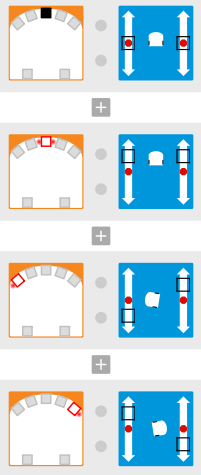
\includegraphics[width=0.3\textwidth]{likes}
\hfill
\begin{minipage}[b]{0.55\textwidth}
\begin{footnotesize}
\begin{verbatim}
onevent prox
    if prox.horizontal[2] < 1000 then
        motor.left.target = 0
        motor.right.target = 0
    end
    if prox.horizontal[2] > 2000 then
        motor.left.target = 300
        motor.right.target = 300
    end
    if prox.horizontal[0] > 2000 then
        motor.left.target = -300
        motor.right.target = 300
    end
    if prox.horizontal[4] > 2000 then
        motor.left.target = 300
        motor.right.target = -300
    end
\end{verbatim}
\end{footnotesize}
\vspace*{8ex}
\end{minipage}
\caption{Ein VPL-Programm mit dem dazugehörenden Text-Programm.}
\label{fig.textcode}
\end{figure}

\p{onevent prox} bedeutet: wann immer die Distanzsensoren ausgewertet werden (Distanzsensoren englisch \emph{proximity} sensors, abgekürzt \emph{prox}), werden die nachfolgenden Befehle bis zur Zeile \p{end} ausgeführt. Die Auswertung erfolgt 10 Mal pro Sekunde. 

Wenn das Ereignis der Auswertung eintritt, werden die Werte der Sensoren abgefragt und mit einer Selektion ausgewertet. Der Sensor mit der Nummer 2 (vorne in der Mitte) wird als erster untersucht: \p{prox.horizontal[2]}. Falls dieser Wert unter 1000 liegt, wird die Geschwindigkeit auf 0 gesetzt mit folgenden Befehlen: 

\begin{footnotesize}
\begin{verbatim}
motor.left.target  = 0
motor.right.target = 0
\end{verbatim}
\end{footnotesize}

Jeder Block \verb+if ... then ... end+ testet einen Sensor und startet die dazu passende Befehlsfolge, falls der Test zutreffend ist. Das Programm folgt dem folgenden Algorithmus: 

\begin{enumerate}[start=0,noitemsep,nosep]
\item Teste, ob nichts vor dem Roboter ist; falls dies zutrifft, hält er an.
\item Teste, ob etwas vor dem Roboter ist; falls dies zutrifft, fährt er voraus.
\item Teste, ob etwas links vor dem Roboter ist; falls dies zutrifft, dreht er sich nach links.
\item Teste, ob etwas rechts vor dem Roboter ist; falls dies zutrifft, dreht er sich nach rechts.
\end{enumerate}

Sobald die Sensoren gelesen wurden und die passende Befehlsfolge gestartet wurde, wartet das Programm auf das nächste \p{prox}-Ereignis, um die Tests erneut zu starten.  Dies wiederholt sich so lange, bis das Programm angehalten wird. 

\sect{Einstellen der Dauer des Timers}

\trickbox{Die Dauer des Timers im Aktions-Block vom Vielfachen von Viertelsekunden (250 ms) bis zu vier Sekunden eingestellt werden.}


\sect{Sensor-Ereignis-Blöcke im Fortgeschrittenen-Modus}

Dieser Abschnitt beschreibt Funktionen der Sensor-Ereignis-Blöcke, die im Fortgeschrittenen-Modus verfügbar sind. 

\subsection*{Einstellen der Schwellenwerte der Sensoren}

Im Standard-Modus sind die Schwellenwerte der Sensoren nicht veränderbar. Für die horizontalen Distanz-Sensoren bedeutet ein Wert oberhalb von 2000, dass viel Licht reflektiert wird und dass das Ereignis eintritt, falls das entsprechende Quadrat weiss ist. Ein Wert von unter 1000 bedeutet hingegen, dass zu wenig Licht reflektiert wird und ein Ereignis eintritt, wenn das entsprechende Quadrat schwarz ist. Für die unteren Sensoren liegen die Werte bei 450 und 400.

Im Fortgeschrittenen-Modus können die Schwellenwerte festgelegt werden. Mit dem oberen Schieber stellt man den Schwellenwert für ein weisses Ereignis ein und mit dem unteren Schieber die Schwelle, unterhalb derer ein schwarzes Ereignis eintritt: \label{p.proximity-sensitivity}

\begin{center}
\begin{tabular}{c@{\hspace{.1\textwidth}}c}
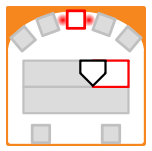
\includegraphics[width=.15\textwidth,keepaspectratio=true]{set-red}
&
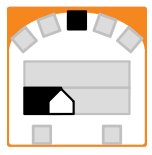
\includegraphics[width=.15\textwidth,keepaspectratio=true]{set-black}
\end{tabular}
\end{center}

\Cref{fig.follow-line-adv} zeigt das Linien-Folgen-Programm (vgl. \cref{fig.follow-line-all}) im Fortgeschrittenen-Modus. Die Schieberegler wurden so eingestellt, dass der Schwellwert sehr tief ist: 100 für den unteren und den oberen Grenzwert.

\begin{figure}
\subfigure[Roboter starten und stoppen]%
{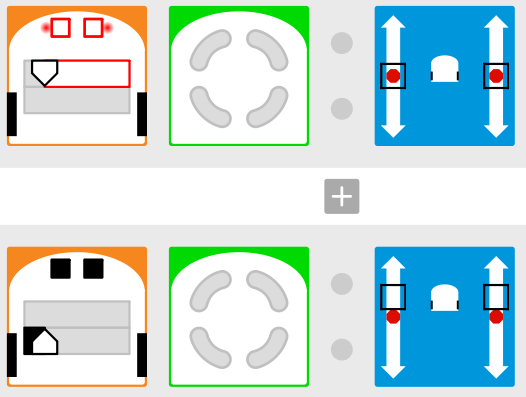
\includegraphics[width=0.45\textwidth]{line-forward-adv}}
\hfill
\subfigure[Korrektur der Abweichung]%
{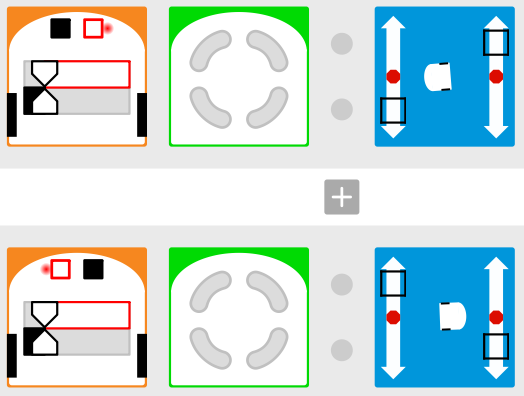
\includegraphics[width=0.45\textwidth]{line-controller-adv}}
\caption{Ein Programm zum Folgen einer Linie}
\label{fig.follow-line-adv}
\end{figure}

\subsection*{Mehrere Sensoren}

Wenn mehrere Sensoren untersucht werden, teilen sie sich die Einstellungen der Schwellwerte:
\begin{center}
\begin{tabular}{c@{\hspace{.1\textwidth}}c}
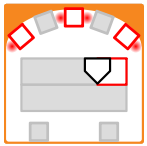
\includegraphics[width=.15\textwidth,keepaspectratio=true]{set-same}
&
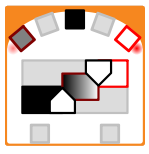
\includegraphics[width=.15\textwidth,keepaspectratio=true]{set-all}
\end{tabular}
\end{center}

\subsection*{Ereignisse für Werte zwischen Grenzwerten}

Im Fortgeschrittenen-Modus gibt es einen zusätzliches Zustand: das Quadrat kann dunkelgrau sein: \gr{set-gray}{.15}
In diesem Zustand tritt ein Ereignis ein, wenn der Wert, der gemessen wurde, zwischen dem oberen und unteren Grenzwert liegt. Der obere Grenzwert wird mit dem oberen Regler festgelegt, der unter mit dem unteren. 

\end{document}
